\RequirePackage[l2tabu, orthodox]{nag}
\documentclass[12pt]{article}
\usepackage[utf8]{inputenc}
\usepackage[T1]{fontenc}
\usepackage{amsmath, amssymb, amsfonts}
\usepackage{newtxtext, newtxmath}
\usepackage{graphicx}
\usepackage{float}
\usepackage[justification=justified]{caption}
\usepackage{subcaption}
\usepackage{booktabs}
\usepackage{microtype}
\usepackage{setspace}
\usepackage{siunitx}
\usepackage[margin=1in]{geometry}
\usepackage{enumitem}
\usepackage[normalem]{ulem}
\usepackage{rotating}
\usepackage{pdflscape}
\usepackage{multicol}
\usepackage[backgroundcolor=orange, linecolor=black]{todonotes}
\usepackage[overload]{textcase}
\usepackage[autostyle=true, english=american, strict=true]{csquotes}
\usepackage[american]{babel}
\usepackage[colorlinks=true, linktoc=all, linkcolor=magenta, citecolor=black, urlcolor=magenta, breaklinks=true]{hyperref}
\usepackage{cleveref}

% \graphicspath{{figures/}}
\graphicspath{{../_figures/}{../docs/panel_files/}}

\setcounter{tocdepth}{3}

\author{Oskar Timo Thoms\\Independent research consultant\\ \\ and Dane Rowlands \& Valerie Percival\\Norman Paterson School of International Affairs}
\title{Lancet-SIGHT Commission Metrics Working Group:\\Report on Large-N and Sequencing Analyses\\(revised with corrections)}
\date{\today\thanks{This report builds and expands on a January 2021 report co-authored with Rowlands and Percival and an interim draft report produced by Thoms in July 2021.}}

\begin{document}

\maketitle
\clearpage
\tableofcontents
\clearpage

\section{Introduction}
\label{intro}

This report summarizes statistical analyses conducted for the Lancet-SIGHT Commission, whose objective is to examine if and how gender equality and health equity can contribute to more peaceful societies.
The central research question is: how does variation in gender equality and health equity -- both improvements and declines -- influence variation in violence and conflict?

The Metrics Working Group explores this question through quantitative analysis of large-N cross-national data, as well as studies based on systematic reviews of the existing literature and the use of descriptive data. First, to understand the quality of the data for both the large-N and the case studies, the Working Group has undertaken a rigorous analysis of indicators used in such research.
Second, through the analysis of a large number of observations, large-N analysis examines associations to determine if and how variables relate to each other and if these relationships have statistical significance, i.e. whether findings of associations are likely not due to chance alone.
Careful statistical analysis can partly account for endogeneity and lessen the chances of spurious associations. Without such large-N analysis, we risk making false causal claims about the generalizability of relationships between gender equality, health equity and peace. In short, large-N analysis can provide greater confidence in the external validity of the Commission's broader analyses.

Inspired by an article by Suri et al (2010), which argues that human development and economic growth operate in vicious and virtuous cycles, we decided to test this concept with three sets of variables on health, gender and violence/conflict. Specifically we want to explore:
if and how gender inequalities and health inequities and violence reinforce each other in vicious cycles;
if and how gender equality, health equity, and peace reinforce each other in virtuous cycles;
and if and how efforts to support gender equality and health equity, under the right conditions, have the ability to nudge communities and societies from vicious to virtuous cycles.

The large-N analyses do not examine the impacts of specific health and gender interventions, but rather begin to build an evidence base for broad statistical relationships between gender, health, and violence outcomes.
Based on the framework proposing that health, gender, and violence variables interact with each other to produce mutually reinforcing negative (vicious) or positive (virtuous) patterns, these analyses are guided by the following questions:
First, while accounting for the overall improvements that almost all countries have experienced in health and gender outcomes in recent decades, do those countries that score low in earlier periods improve less than the global average and/or high performers, or do they perhaps even decline?
Second, while accounting for possible ceiling effects, do those countries that score high in earlier periods a) maintain stable and high levels and b) avoid violence?
Third, do countries that experience higher levels of violence a) improve less on gender equality and health outcomes than those with less violence, or b) do their gender and health outcomes perhaps even deteriorate?
Fourth, are countries that score low on health and gender outcomes more prone to violence than those that score higher?

These questions imply considerable complexity, as they examine statistical effects between gender and health outcomes; from gender and health outcomes to violence; and from violence to gender and health outcomes.\footnote{
While the Lancet-SIGHT Commission is primarily interested in the direction of effects from gender and health to violence, the virtuous and vicious cycles framework implies feedback loops.}
The bivariate descriptive and multivariate regression analyses discussed in this report examine these questions in probabilistic terms, not in deterministic fashion.
While there are many other important factors influencing health, gender and violence outcomes, we do not develop detailed causal models of each outcome, but examine whether statistical associations between the three categories of outcomes are consistent with the theoretical framework. We see this exploratory research as a first useful step in a larger research agenda exploring relationships between health, gender, and peaceful societies. We steer clear of causal language to describe the results because no strong causal claims can be made on the basis of these analyses, but we find associations -- some stronger and some weaker -- that are consistent with the proposed framework and that warrant deeper investigation. Therefore, we consider this work to be useful ground-clearing for establishing a new research agenda on the inter-relationships between health, gender and violence.

We examined multivariate models of both cross-sectional and panel data. These two different approaches to modeling cross-national data have complementary advantages and disadvantages.
The cross-sectional models allow us to examine long-term changes in the outcome variables, over twenty-year periods, while the panel models examine short-term variation, from one five-year period to the next but over longer time-frames than the cross-sectional analyses.
The two approaches have different methodological trade-offs. While the cross-sectional models make it somewhat easier to address problems of endogeneity and heteroscedasticity, they also have fewer degrees of freedom due to their small sample sizes, i.e. the number of countries included. Panel models are subject to more concerns about endogeneity, heteroscedasticity and serial correlation due to the structure of the data used, i.e. several observations of countries over time, but they also have much larger sample sizes allowing for more precision in statistical estimates. We believe that both approaches are valuable in examining the research questions.

Two previous reports presented key elements of the cross-sectional and panel analyses.
The first (January 2021) presented the initial analyses, finding some support for virtuous and particularly vicious cycles, while the second (July 2021) extended the panel analyses to address questions that emerged with respect to the operationalization of vicious and virtuous cycles, the robustness of results, and some differences in findings between the cross-sectional and panel analyses.
All analyses in the present report have been revised and supersede those of the earlier work.

Finally, in addition, this report presents descriptive analyses of sequences of health and gender change.
The Lancet-SIGHT Commission is interested not only in whether vicious and virtuous cycles are at work, but also if and how policy interventions to support gender equality and health equity can nudge societies into virtuous cycles.
Toward this end, it is useful to examine pathways of gender and health change to identify entry points and policy levers.
A key question is: are there particular sequences of improvements in gender and health outcomes that are more likely to break countries out of vicious cycles?
An important first step is to map different pathways of change in health and gender over time, to determine which pathways are more common than other and which ones are more likely to lead to improvements.

The remaining sections cover the three sets of analyses.
\Cref{data} discusses the data used throughout all analyses.
\Cref{cross-sectional}, authored by Dane Rowlands, presents the cross-sectional analyses.
The remaining two sections were produced by Oskar Timo Thoms.
\Cref{panel} discusses the methods and results of the panel analyses.
Finally, \Cref{sequencing} presents the methodology used in mapping pathways and coding a typology of sequences, and presents basic descriptive analyses of these new data.

% \todo[inline]{needs a brief paragraph here previewing the overall main findings}

\clearpage
\section{Data}
\label{data}
\paragraph{Oskar Timo Thoms}

\subsection{Variables used in the analyses}
\label{variables}

Guided by the indicator mapping carried out by the Metrics Working Group, we identified a wide range of health, gender and violence measures as candidates for analyses, and assembled a comprehensive cross-national time-series dataset with the best available data on relevant indicators and key covariates.\footnote{
A detailed codebook is available at this \href{https://docs.google.com/spreadsheets/d/1KLFTva--XHVBM-IX6qaPtuyzmIlRMnpyjUXfBdJPsag/edit?usp=sharing}{link}.}
Many health and gender measures in particular are subject to many missing data points across countries and over time, and this missingness is unlikely to be random and thus presents a potential threat to inferences. Therefore, based on our evaluation of the quality and coverage of these data, and based on within-category correlations, for the main analyses we chose two representative and commonly accepted variables each for the health (life expectancy and the IMR) and gender (the mean years of schooling ratio of females to males and the age-specific fertility rate for adolescents, AFR) dimensions.\footnote{
Details on data coverage and correlations are available at \href{https://timothoms.github.io/LSC-MWG/}{timothoms.github.io/LSC-MWG/data.html}.}

In robustness checks, the panel analyses also examine whether statistical associations hold for other outcomes, by substituting other health (under-five mortality rate, UFMR, and disability-adjusted life years, DALYs) and gender measures (the labour participation ratio of females to males and the Gender Inequality Index, GII) as the dependent variables. These additional measures are chosen based on data availability and to expand the conceptual range of the gender and health dimensions.
To measure violence, we chose several indicators to capture different types, including state-based internal armed conflict, state repression and societal violence, and the total and civilian battle-related death rates per population resulting from varying types of conflict, and homicide rates.

\begin{table}[h]
\footnotesize
\centering
\caption{Measures used in the large-N analyses}
\label{table_vars}
\begin{tabular}{llrr}
\toprule
Category             & Variable                                                 & Source             & available from\\
\midrule
health               & life expectancy                                          & WPP                & 1950 \\
                     & \textbf{\textit{infant mortality rate}} (IMR)            & WPP                & 1950 \\
                     & \textbf{\textit{under-five mortality rate}} (UFMR)       & WPP                & 1950 \\
                     & \textbf{\textit{disability-adjusted life years}} (DALYs) & IHME               & 1990 \\
gender               & mean years of schooling (MYS) ratio                      & IHME               & 1970 \\
                     & \textbf{\textit{adolescent fertility rate}} (AFR)        & WPP                & 1950 \\
                     & labour participation ratio                               & ILO                & 1990 \\
                     & Gender Inequality Index (GII)                            & HDR                & 1995 \\
state-based conflict & internal (incl. internationalized) conflict incidence    & UCDP               & 1946 \\
                     & internal (incl. internationalized) war incidence         & UCDP               & 1946 \\
                     & internal conflict deaths (rate per pop.)                 & UCDP               & 1989 \\
                     & internal conflict civilian deaths (rate per pop.)        & UCDP               & 1989 \\
state repression     & one-sided violence (OSV) incidence                       & UCDP               & 1989 \\
                     & one-sided violence (OSV) deaths (rate per pop.)          & UCDP               & 1989 \\
                     & \textbf{\textit{latent physical integrity measure}}      & Chris Fariss       & 1946 \\
                     & \textbf{\textit{state torture}}                          & V-Dem              & 1789 \\
                     & \textbf{\textit{extra-judicial killings}}                & V-Dem              & 1789 \\
societal violence    & non-state conflict (NSC) incidence                       & UCDP               & 1989 \\
                     & non-state conflict (NSC) deaths (rate per pop.)          & UCDP               & 1989 \\
                     & non-state conflict (NSC) civilian deaths (rate per pop.) & UCDP               & 1989 \\
                     & homicides (rate per pop.)                                & ODC/WHO            & 1990 \\
controls             & population size (logged)                                 & WPP                & 1950 \\
                     & real GDP per capita (logged)                             & PWT                & 1950 \\
                     & electoral democracy index                                & V-Dem              & 1789 \\
                     & participatory democracy index                            & V-Dem              & 1789 \\
                     & polity 2 index                                           & CSP Polity Project & 1800 \\
\bottomrule
\end{tabular}
\end{table}


These variables are listed in \Cref{table_vars}.\footnote{
The panel analyses for the first report included measures of internal war and state torture. This report does not discuss any panel analyses using these two measures because the initial results were very similar to those for internal conflict and extra-judicial killings, respectively.} Some of these data are available for earlier years, but as the IHME educational data is available from 1970 onward, this is the starting point for our initial dataset.
Moreover, the OSV, NSC and all the death rates derived from the Uppsala Conflict Data Programme (UCDP) are available from 1989. Finally, the DALYs, labour participation ratios, and GII data are only available from 1990, 1990, and 1995, respectively.
Thus, the samples in analyses using these latter variables are more limited.
All variables are aggregated to five-year averages (covering 1971-75, 1976-1980, etc.) because three of the key health and gender variables are provided as such averages by the World Populations Prospects (WPP) database.
As data availability and quality generally improves after 1989 and more violence variables exist for this period, the primary period of the analyses is 1991-2015, with some variation depending on the variables included.

It is important to note that, for easier comparisons of results across variables within the health, gender and violence dimensions, \textbf{we have inverted some variables for the statistical analyses such that higher values of all health and gender variables always indicate \enquote{better} outcomes, while higher values of the violence variables always mean higher levels of violence}; the affected variables are indicated by \textbf{\textit{bold italics}} in \Cref{table_vars}. Readers familiar with these measures should keep in mind that this alters how one would usually interpret the results.

For control variables, we use per capita income to represent the level of a country's economic development, population size, and measures of political structure representing the presence or absence of facets of democracy. While not exhaustive, these variables exhibit useful features in terms of country and year coverage, collection and reporting reliability, and theoretical plausibility. For political factors, the panel models reported only include a measure of participatory democracy, as this was the only measure of political structures that consistently showed significant associations in initial analyses.

\subsection{Classifications to operationalize vicious and virtuous cycles}
\label{classifications}

\begin{sidewaystable}
\footnotesize
\centering
\caption{Country classifications in 1995 (for 1975, see \Cref{class1975}).}
\label{class1995}
\begin{tabular}{p{0.04\linewidth} p{0.175\linewidth} p{0.175\linewidth} p{0.175\linewidth} p{0.175\linewidth} p{0.175\linewidth}}
\toprule
\multicolumn{1}{l}{} & \multicolumn{5}{l}{\textbf{Gender}} \\
\textbf{Health} & Q1 & Q2 & Q3 & Q4 & Q5\\
\midrule
Q1 & Afghanistan; Angola; Benin; Burkina Faso; Cameroon; Central African Republic; Chad; Congo, DRC; Cote d'Ivoire; Equatorial Guinea; Eritrea; Ethiopia; Guinea; Guinea-Bissau; Liberia; Malawi; Mali; Mozambique; Niger; Nigeria; Sierra Leone; Somalia; Tanzania; Uganda; Zambia & Burundi; Cambodia; Haiti; Laos; Madagascar; Rwanda &  &  & \\
\hline
Q2 & Bangladesh; Bhutan; Comoros; Congo; Gambia; Nepal; Pakistan; Sao Tome \& Principe; Senegal; Sudan; Togo; Yemen & Bolivia; Djibouti; Egypt; Eswatini; Gabon; Ghana; Guatemala; India; Kenya; Maldives; Mauritania; Papua New Guinea; Zimbabwe & Botswana; Indonesia; Kiribati; Myanmar; Namibia; Tajikistan & Azerbaijan; Mongolia; Turkmenistan & Lesotho\\
\hline
Q3 &  & Belize; Cape Verde; Honduras; Iran; Iraq; Morocco; Nicaragua; Oman; Palestinian Territory; Saudi Arabia; Solomon Islands; Turkey & Algeria; Armenia; Brazil; China; Dominican Republic; Ecuador; El Salvador; Fiji; Guyana; Jordan; Kyrgyzstan; Libya; Micronesia; Paraguay; Peru; South Africa; Suriname; Tunisia; Uzbekistan; Vanuatu; Viet Nam & Georgia; Kazakhstan; Moldova; North Korea; Philippines; Russian Federation; Trinidad \& Tobago & Latvia; Samoa\\
\hline
Q4 &  & Syria & Colombia; Grenada; Jamaica; Macedonia; Mauritius; Mexico; Panama; Saint Lucia; Saint Vincent \& the Grenadines; Thailand; United Arab Emirates; Venezuela & Albania; Antigua \& Barbuda; Argentina; Bahamas; Bahrain; Bosnia \& Herzegovina; Brunei; Bulgaria; Chile; Croatia; Czech Republic; Kuwait; Lebanon; Lithuania; Malaysia; Romania; Seychelles; Slovakia; South Korea; Sri Lanka; Ukraine; Uruguay & Belarus; Estonia; Hungary; Poland; Tonga\\
\hline
Q5 &  &  & Costa Rica; Cuba & Barbados; Cyprus; Qatar; Singapore; Taiwan; United States of America & Australia; Austria; Belgium; Canada; Denmark; Finland; France; Germany; Greece; Iceland; Ireland; Israel; Italy; Japan; Luxembourg; Malta; Netherlands; New Zealand; Norway; Portugal; Slovenia; Spain; Sweden; Switzerland; United Kingdom\\
\bottomrule
\end{tabular}
\end{sidewaystable}


Vicious and virtuous cycles can be conceptualized and operationalized in different ways.
The simplest tests are whether the individual gender and health variables are positively correlated with each other or with violence variables, controlling for other factors.
While we include such models, this approach comes with two distinct drawbacks.
First, these correlations between two variables imply that vicious and virtuous cycles are simply two sides of the same coin -- one implies the other.
This approach cannot distinguish between vicious and virtuous cycles, and allow for the possibility that one could occur without the other or that they operate on different timelines.
Second, in this approach, it is not possible to determine whether the gender, health and violence variables actually mutually reinforce each other, i.e. whether their combinations have statistical effects beyond their individual effects.
Such effects could be investigated with two-way or even three-way interaction terms between the health, gender and violence variables in the statistical models, but this approach quickly becomes very complicated to implement and interpret.
To make the analyses more tractable, we opt for an approach using joint classifications, which is akin to including interaction terms.

\begin{table}
\centering
\caption{Frequency of classifications in 1995 (181 countries; for 1975, see \Cref{class1975n}).}
\label{class1995n}
\begin{tabular}{lccccc}
\toprule
                & \multicolumn{5}{l}{\textbf{Gender}} \\
\textbf{Health} & 1st quintile & 2nd quintile & 3rd quintile & 4th quintile & 5th quintile \\
\midrule
1st quintile    & 25           & 6            & 0            & 0            & 0 \\
2nd quintile    & 12           & 13           & 6            & 3            & 1 \\
3rd quintile    & 0            & 12           & 21           & 7            & 2 \\
4th quintile    & 0            & 1            & 12           & 22           & 5 \\
5th quintile    & 0            & 0            & 2            & 6            & 25 \\
\bottomrule
\end{tabular}
\end{table}


We developed a classification of countries based on the four main health and gender outcomes, in order to create groups of countries for comparisons.
For each five-year period, we standardized each of the four measures such that they have zero means and standard deviations of one.
We then took the averages of the two health measures and of the two gender measures, and divided the resulting combined health and gender measures into quintiles to produce a 5x5 matrix for each five-year period.
For instance, for the period ending in 1995, this leads to the country classifications shown in \Cref{class1995} and the cell frequencies shown in \Cref{class1995n}. (The appendix also shows tables for the period ending in 1975.) These tables suggest a strong correlation between the standardized health and gender outcomes, as most countries are classified on the diagonal. Off-diagonal classifications are less common.

\begin{table}[htb]
\centering
\caption{Classification categories used in the analyses}
\label{table_class}
\begin{tabular}{lccccc}
\toprule
                & \multicolumn{5}{l}{\textbf{Gender}} \\
\textbf{Health} & 1st quintile & 2nd quintile & 3rd quintile & 4th quintile & 5th quintile \\
\midrule
1st quintile    & low & low & G>H & G>H & G>H \\
2nd quintile    & low & low & G>H & G>H & G>H \\
3rd quintile    & H>G & H>G & mid & G>H & G>H \\
4th quintile    & H>G & H>G & H>G & upp & upp \\
5th quintile    & H>G & H>G & H>G & upp & upp \\
\bottomrule
\end{tabular}
\end{table}


To make these classifications amenable to statistical analysis, we further aggregate them into five groups for inclusion in some of our statistical models, as in \Cref{table_class}: the lower, middle, and upper diagonal classification groups, where countries have similar relative health and gender outcomes, and those that score comparatively higher on health than on gender ({H>G}), and those that score comparatively higher on gender than on health ({G>H}).\footnote{
Initially, we used only the bottom four cells as our low classification and the top four as our upper classification, making the assumption that if there are virtuous and vicious cycles present, then they surely would be observed for these two groups. While this expectation was borne out in some models, it also became clear that the large middle category lumped together much potentially interesting variation. Therefore, we introduced the distinction for off-diagonal cells, to explore the possibility that vicious and virtuous cycles could also be at work in the middle.}

\begin{figure}
    \centering
    \caption{Average life expectancy trends}
    \label{trends_life expectancy}
    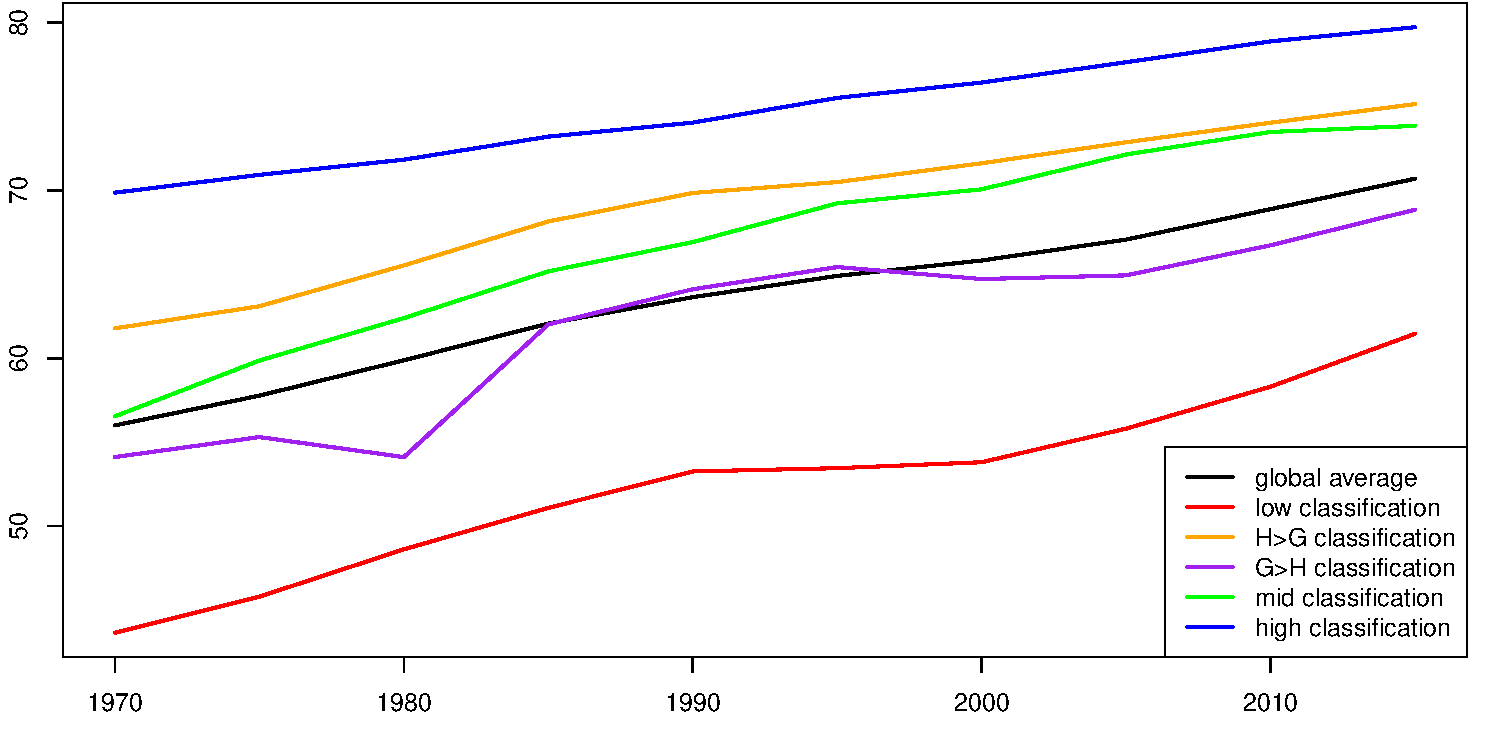
\includegraphics[width=\textwidth]{figures/trend_life_exp_wpp.pdf}
\end{figure}
\begin{figure}
    \centering
    \caption{Average infant mortality trends}
    \label{trends_imr}
    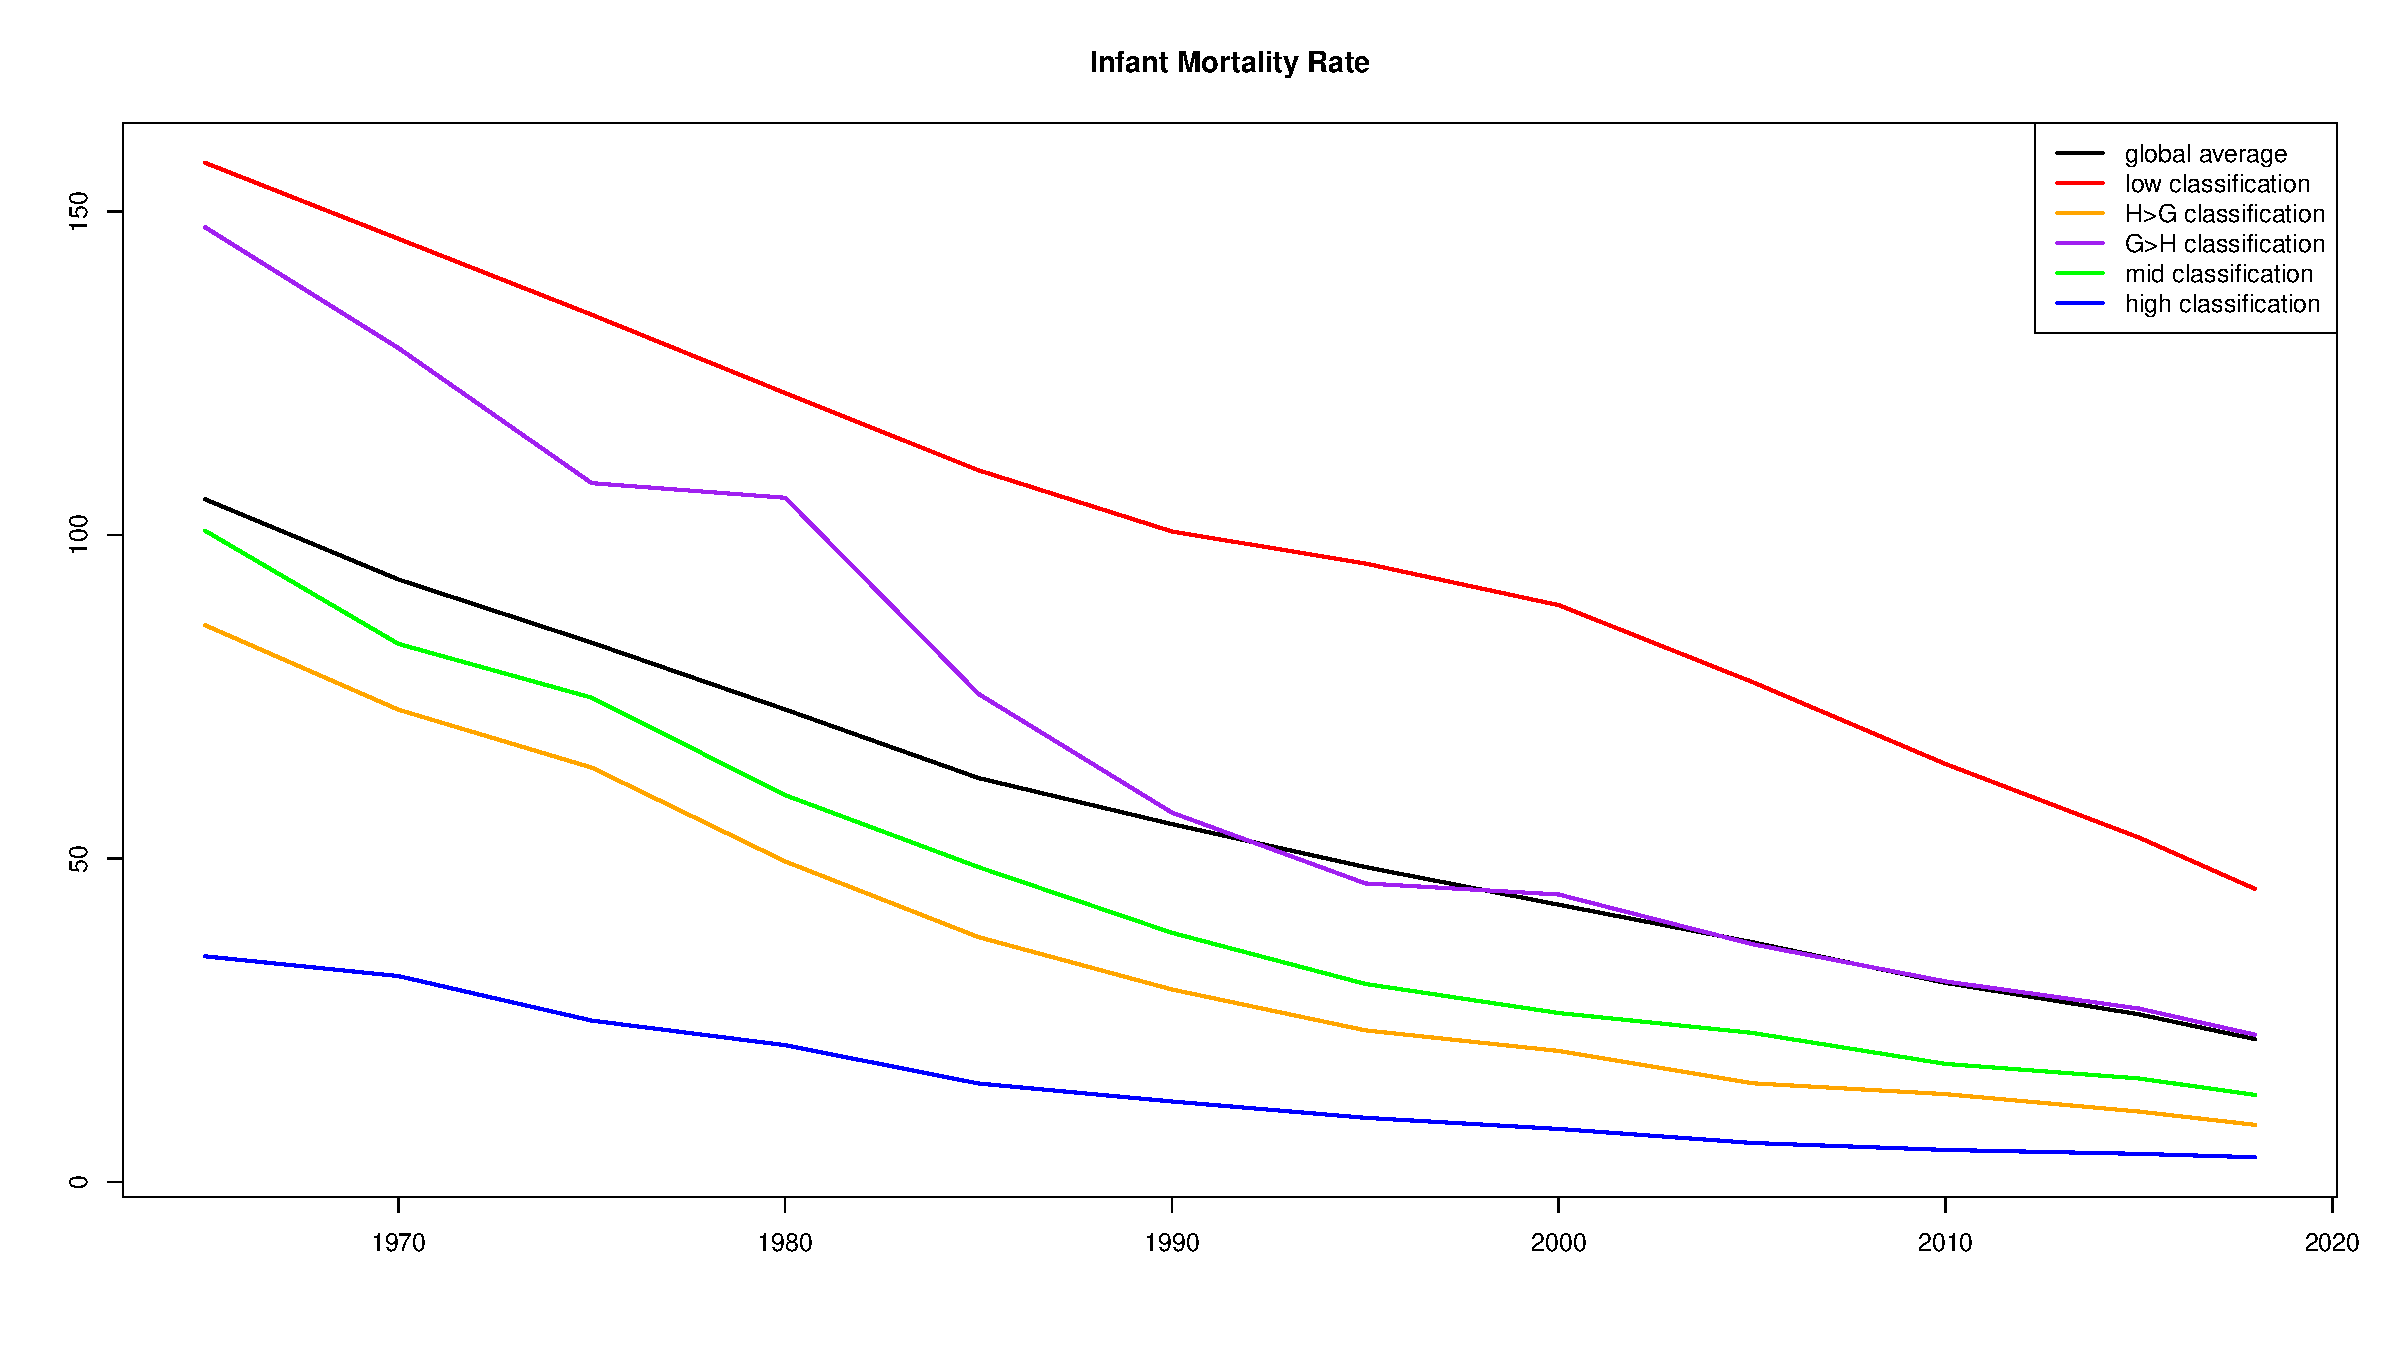
\includegraphics[width=\textwidth]{figures/trend_imr_wpp.pdf}
\end{figure}
\begin{figure}
    \centering
    \caption{Average mean years of schooling ratio trends}
    \label{trends_mys}
    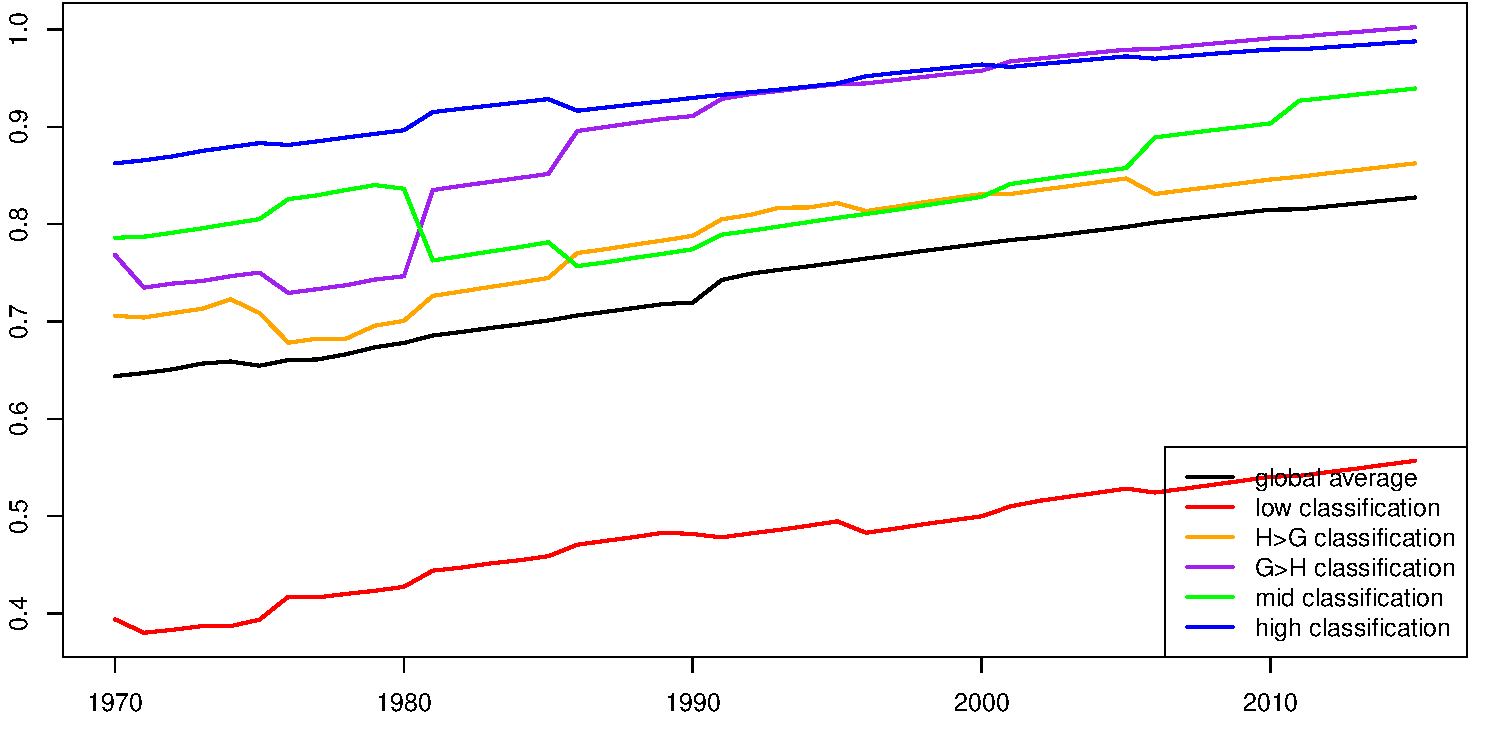
\includegraphics[width=\textwidth]{figures/trend_mys_age_ratio_ihme.pdf}
\end{figure}
\begin{figure}
    \centering
    \caption{Average adolescent fertility trends}
    \label{trends_afr}
    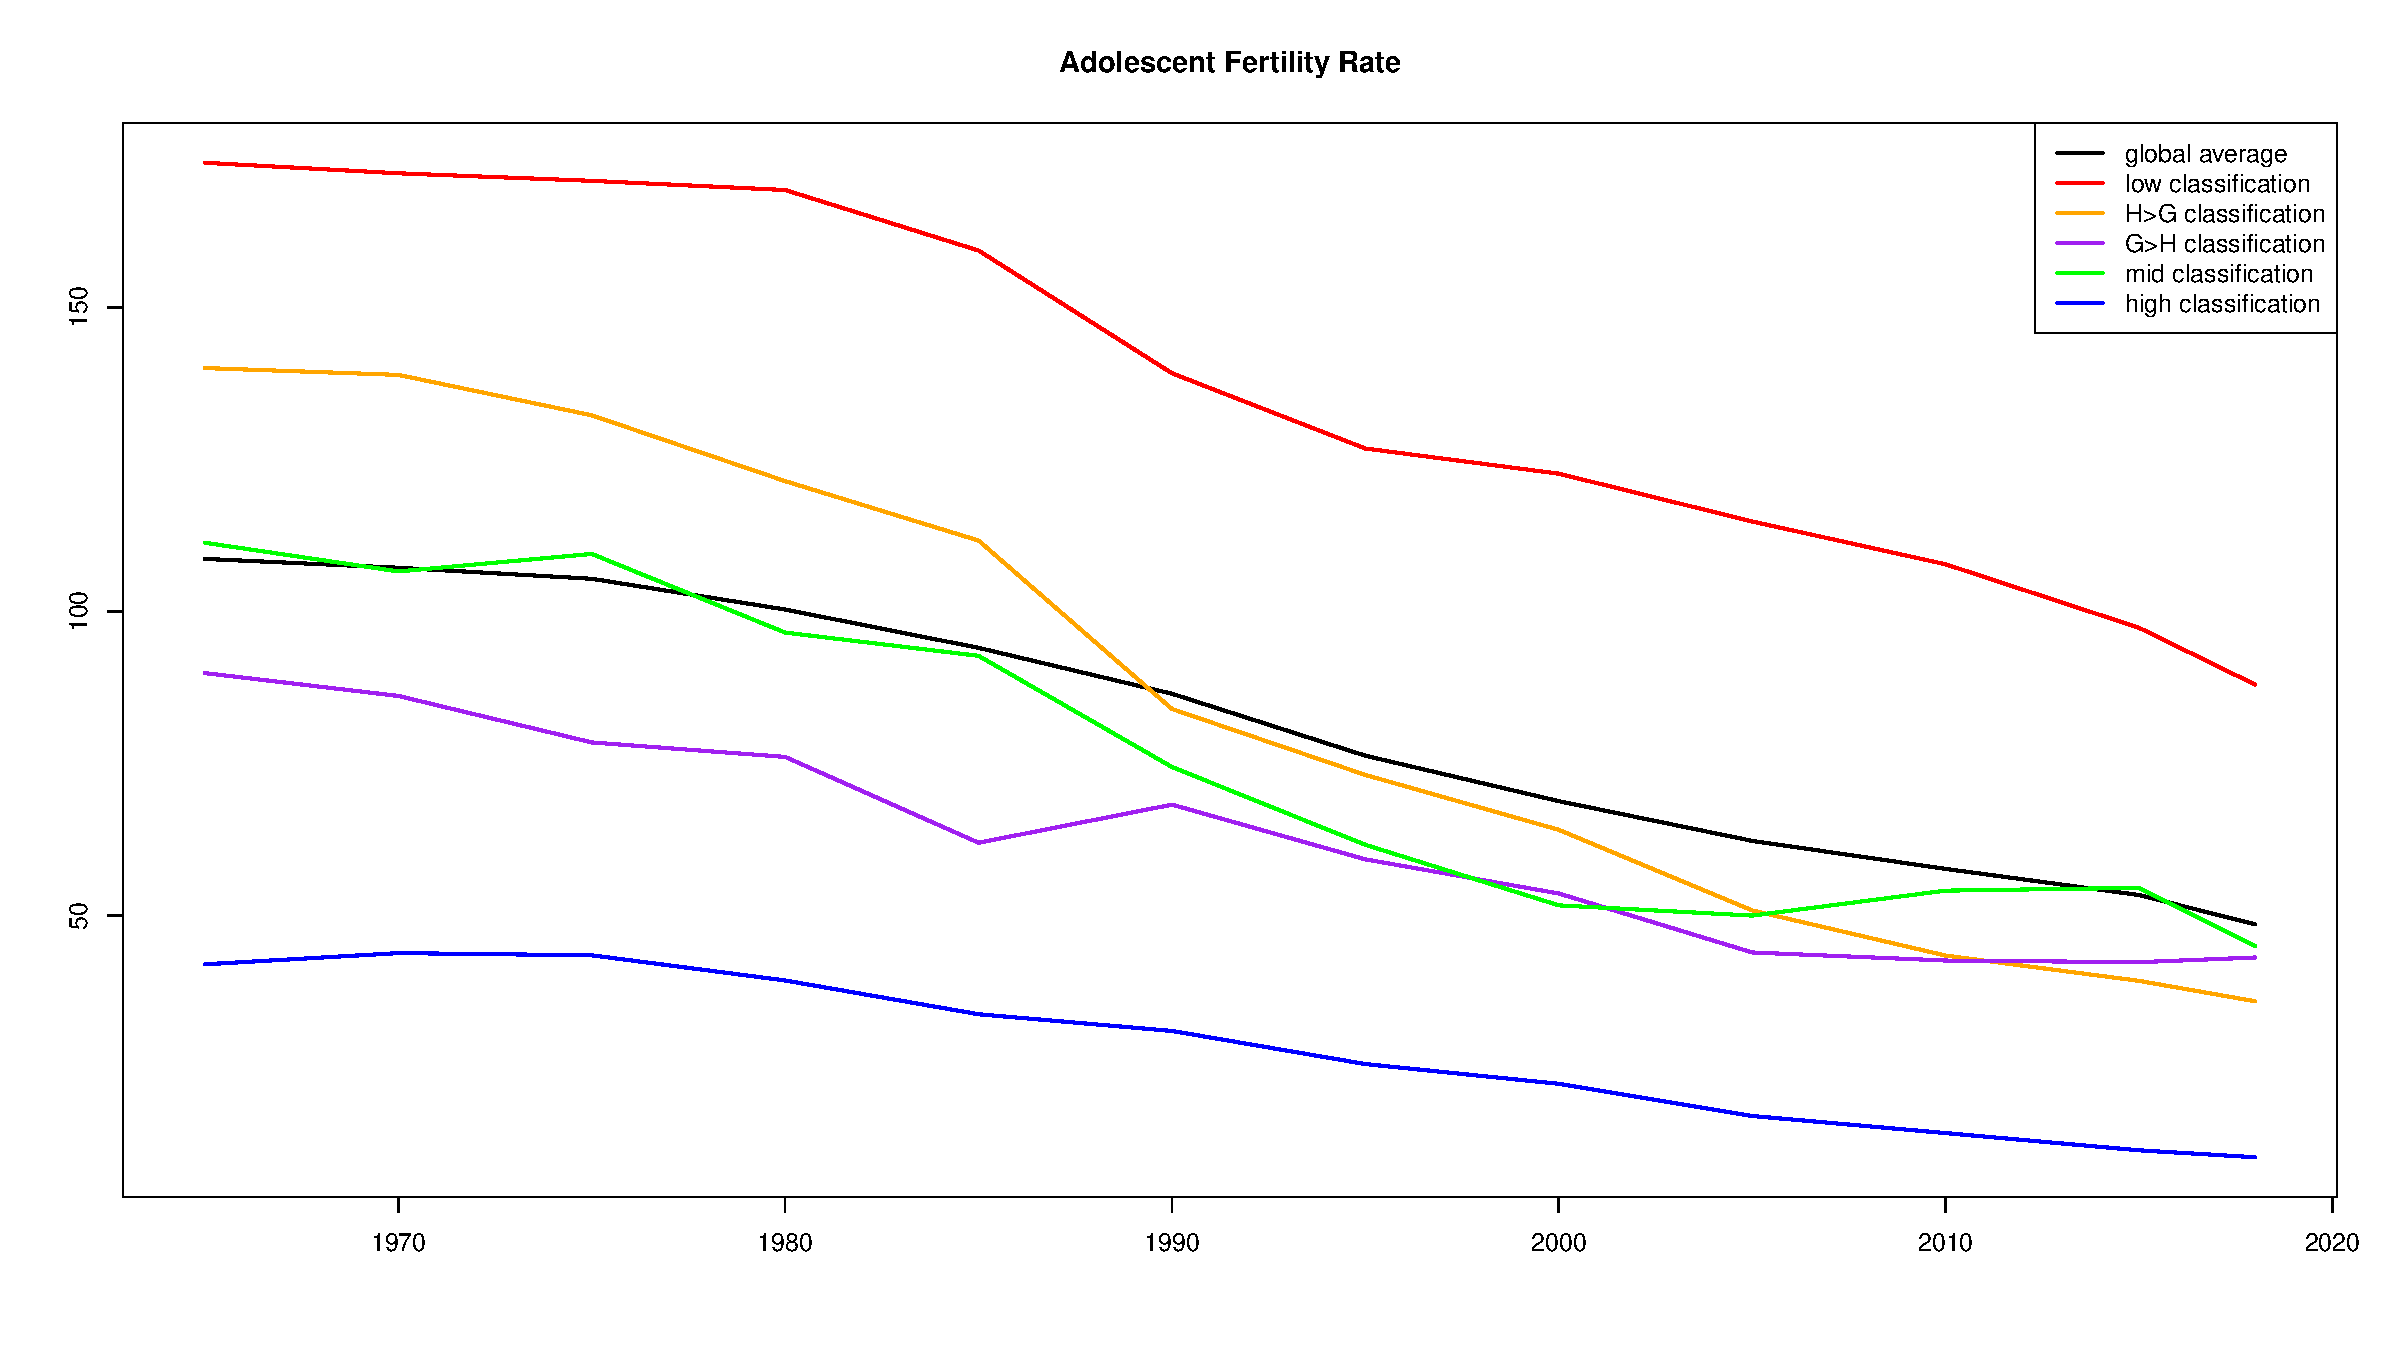
\includegraphics[width=\textwidth]{figures/trend_asfr_adol_wpp.pdf}
\end{figure}

Plotting the averages of the four health and gender variables at the global level (the gray lines) and within the classification groups in Figures \ref{trends_life expectancy}-\ref{trends_afr} shows clear trends over time.
Note that these figures show the original measures as five-year averages, not the inverted versions used in the statistical analyses below.
These figures support two important points.
First, there is considerable global improvement in the health and gender measures, regardless of how countries are classified.
Second, overall improvements are greatest in the low classifications, with some interesting differences. Most improvement in the IMR occurs in the {G>H} classification, and most improvement in the AFR occurs in the {H>G} classification, followed by the low classification.
Improvements tend to be much less pronounced in the upper classification.
These trends suggest ceiling effects for better performers; those that start out at relatively low levels of health and gender outcomes have much more room to improve.

The classification groups are used in the analyses below to examine the possibility of vicious and virtuous cycles in two different ways.
First, to examine whether particular configurations of health and gender outcomes (i.e. the classification groups) are associated with improvement or worsening in gender, health and violence variables, we include models with binary (\enquote{dummy}) variables indicating the groups in \Cref{table_class}. This can be interpreted as the effect of past health and gender configurations on current health and gender outcomes or on violence outcomes, relative to one excluded or reference category in the classification.
Associations of lower classifications with worse outcomes and of higher classifications with better outcomes would provide evidence that is consistent with \enquote{two-way} vicious or virtuous cycles, respectively.

Second, modelling interactions of these binary classification indicators with violence variables lets us calculate the statistical effects of past violence within each classification group on current health, gender or violence outcomes. This can be interpreted as a \enquote{three-way} cycle. We can test whether past violence in particular classification groups is associated with worse or better current health or gender outcomes or with more or less violence. For instance, if we find an association of past violence in lower classifications with more current violence or worse health or gender outcomes, this evidence would support vicious cycles because violence limits health or gender improvements or begets more violence where countries already perform comparatively poorly on health and gender. Or, if we find past violence in higher classifications groups is associated with better health or gender outcomes or less violence, this would support virtuous cycles, because countries in the higher classifications were able to maintain or improve outcomes despite the violence. Moreover, the evidence does not need to be this clear-cut to be supportive of vicious and virtuous cycles. Rather, the relative statistical effects of past violence in the different classification groups may be consistent with such cycles.
For instance, past violence may be associated with more current violence across several or all classifications, but more so in lower classifications relative to higher ones; such evidence would be supportive of vicious cycles.

\subsection{Bivariate associations}

Other graphical analyses of bivariate associations not shown here indicate that low performers on the health and gender dimensions tend to have the most violence on average over time (across different measures and different types of violence), and high performers experience much less violence.\footnote{
These figures are available at \href{https://timothoms.github.io/LSC-MWG/}{timothoms.github.io/LSC-MWG/data.html}.}
In a partial exception to this strongly supported generalization, average homicide rates are highest in the intermediate rather than the low classifications, but the upper classification still clearly has the lowest average homicide rates.

\begin{figure}[htb]
    \centering
    \caption{Internal (\& internationalized) conflict (1996-2015) by 1995 classification}
    \label{class1995conflict}
    \includegraphics[width=\textwidth]{figures/class_conflict_1995_1996.pdf}
\end{figure}

We only show the bivariate relationship between the classification groups and internal conflicts, as this is of particular interest to the Lancet-SIGHT Commission, and it illustrates the strong bivariate relationship between joint gender and health outcomes on one side and violence on the other.
\Cref{class1995conflict} distinguishes countries that during the period 1996-2015 had any conflict (based on a threshold of 25 battle-related deaths in a given year) or war (based on a threshold of 1000 battle-related deaths in a given year) and whether countries had such conflict or war for five years or more over the entire period.
% \footnote{The conflict variable is coded from the UCDP Armed Conflict Dataset version 20.1.}
While the majority of countries in each classification group had no conflict, the proportion (i.e. the ratio between \enquote(none) and all the conflict categories) is lowest in the low and G>H classifications and highest in the upper classification. Moreover, the lower the classification, the higher the proportion of countries with five or more years of conflict and/or wars with high death counts per year.

\begin{figure}[htbp]
    \centering
    \caption{Internal (\& internationalized) conflict (1996-2015) by 1995 classification}
    \label{class1995conflict_pre}
    \begin{subfigure}[b]{\textwidth}
      \caption{no previous conflict (1976-1995)}
      \includegraphics[width=\textwidth]{figures/class_conflict_1995_1996_prenone.pdf}
    \end{subfigure}
    \begin{subfigure}[b]{\textwidth}
      \caption{at least one previous conflict (1976-1995)}
      \includegraphics[width=\textwidth]{figures/class_conflict_1995_1996_presome.pdf}
    \end{subfigure}
\end{figure}

When the conflict data for 1996-2015 are further broken down in \Cref{class1995conflict_pre} by whether a country had internal conflict or war in the previous twenty years (1976-1995), another important observation can be made.
Among countries that had no previous conflict or war, very few had any conflict in 1996-2015 and most of these occurred in the low classification group.
However, when considering only those countries that had at least one conflict-year in 1976-1995, the differences between the lower and higher classifications are particularly stark: almost four out of five countries in the low and G>H classification groups had internal conflict or war again, and three out of five in the H>G classification group. Countries in the mid classification were least likely to experience conflict again.
Thus, internal conflict in the past is strongly associated with internal conflict in the future, and overwhelmingly so for those countries placed lower in our classification based on health and gender outcomes.

On their face, these data are strongly consistent with the vicious and virtuous cycles hypothesis and they provide cause for deeper analyses. However, bivariate associations are inherently limited in that they do not account for plausible alternative explanations and endogeneity and selection effects.
They could represent spurious associations and must not be interpreted as causal.
The multivariate analyses in the next two sections begin to further probe the statistical relationship.

\section{Cross-sectional analyses}
\label{cross-sectional}
\paragraph{Dane Rowlands}\ \bigskip

For the first part of the large sample empirical analysis we use national-level cross-sectional data to test the hypothesis that health, gender, and violence interact in ways that generate mutually reinforcing positive (virtuous) or negative (vicious) patterns. Building on the extensive collection, review and evaluation of different cross-country variables, we select two measures to represent basic health performance (life expectancy and infant mortality rates), two to represent gender equality (the ratio of female-to-male mean years of schooling, and the age-specific fertility rate for adolescents) and a variety of measures of conflict and violence. For controls, we also use per capita income to represent the level of a country’s economic development, and a basic measure of political structure (polyarchy). While not exhaustive, these variables exhibit useful features in terms of country and year coverage, collection and reporting reliability, and theoretical plausibility. We use regression analysis to examine the associations between these variables. The analysis unfolds in a series of accumulating steps to explore different potential interactions amongst our set of variables.

There are a few important observations on the data that need to be recognized. First, on average, most of the key indicators of health and gender exhibit steady improvement over the 1995-2015 period both in average and for almost all countries in the sample. As a result, in the cross-section analysis, virtuous circles and vicious circles are essentially opposite sides of the same coin as the performance of countries are measured relative to one another.\footnote{
One line of inquiry that might be worth pursuing is to impose an absolute measure, for example sustained declining performance, and ask which country groups exhibit absolute decline. In the cross section data it is rare that well-off countries end up having sustained reduction in health and gender performance, while poorly-off countries exhibit a much broader range of future performance, ranging from sustained declines to dramatic improvements.}

% \todo[inline]{Dane: Timo...could we get a quick calculation of the \% of global population we are including in our biggest sample? It might be a useful addition here to emphasize the extent of our sample.}

Data are collected on 201 territorial entities, and while missing information restricts this number in the regressions, we are still able to analyze a very large group of countries with extensive global coverage. The largest sample in the cross-section analysis is 180 countries. Most of the missing 21 jurisdictions are states that had ceased to exist (e.g. the Soviet Union), had only recently been formed (e.g. Kosovo) or were very small states (e.g. Palau).\footnote{\label{fn2}
The full list of missing countries in the largest sample is: Andorra, Czechoslovakia, Dominica, East Germany, Kosovo, Liechtenstein, Marshall Islands, Macau, Montenegro, Nauru, Palau, Saint Kitts \& Nevis, San Marino, Serbia,
Serbia \& Montenegro, South Sudan , Soviet Union, Timor-Leste, Tuvalu, West Germany, Yugoslavia SFR. The additional exclusions are Afghanistan, Antigua \& Barbuda, Bahamas, Belize, Brunei, Cuba, Eritrea, Grenada, Kiribati, Libya, Micronesia, Papua New Guinea, Saint Lucia, Saint Vincent \& the Grenadines, Samoa, Solomon Islands, Somalia, Tonga, Vanuatu.}
The smallest sample in the analysis is 161 countries, which unfortunately excludes some failed states that would be useful as extreme cases of possible vicious cycles (Afghanistan and Somalia, for example). Overall, the sample is biased against small (especially island) states, states that have fallen apart or become recently formed, those in extreme distress, and some that have largely been excluded from parts of the international system of data collection (Cuba). Since these exclusions are clearly non-random, our results should not be taken as necessarily universal.

% \input{tables/cs_descriptives.tex}
% \todo[inline]{insert descriptives table here}

In terms of the standard regression diagnostics, the analysis pays particular attention to problems of multicollinearity, as we know that many of these variables are closely associated theoretically and empirically. We adjust estimating models accordingly, and specifically avoid using the life expectancy and infant mortality performance in the same equation as their correlation coefficient is very high ($\rho = 0.96$).  By contrast, the two measures used for gender equity have a correlation coefficient of only 0.6 and their joint inclusion in models is not particularly problematic. In addition, preliminary tests indicate that all estimating equations exhibit heteroscedasticity, and so models are estimated with robust standard errors.

\subsection{The effects of health and gender conditions on their future improvement}

We start with an analysis of the most basic possible structure relating our four health and gender condition measurements in 1995 with their improvements over the subsequent 20 year period of 1996-2015. The underlying framework is one of direct effects of current values on their future changes as shown in the figure below.

\subsubsection*{(i) direct virtuous or vicious effects version 1}

\begin{equation*}\begin{gathered}
\text{Initial health and gender conditions} \\
\longrightarrow \\
\text{Subsequent long-term improvements in health, gender, and conflict levels}
\end{gathered}\end{equation*}
\bigskip

For this first step we used improvements in each health and gender measure as the dependent variable, and the 1995 values as the regressors. The results are presented in \Cref{cs_table1} from which we draw four key observations.\footnote{
Initial diagnostic tests indicated that the regressions violated the assumption of homoscedasticity, so all p-values are calculated on the basis of robust standard errors. Variance inflation factor (VIF) tests also indicated extensive multicollinearity. Reported models drop variables with statistically insignificant coefficients in a stepwise manner until multicollinearity problems are minimized and sample size is maximized. Models were re-run several times to drop variables associated with multicollinearity in order to ensure that reported results are reasonably stable.}
First, global coverage is extensive, with 180 countries appearing in the sample (see \Cref{fn2}). Second, the associations between the variables are fairly strong, with goodness of fit measures ($R^2$) ranging from a high of 0.82 (for infant mortality) to a low of 0.25 (education equality). Third, high achievement in the initial level of each measure is negatively associated with its subsequent improvement. We attribute this to the presence of a strong ceiling effect by which the rate of improvement of a variable will decline the closer a country already is to the best performance. For example, there are biological and technological limits to how long a person may live or how low infant mortality or adolescent fertility rates can go, and the marginal cost of achieving a unit of improvement will rise as achievements improve. Finally, there is some evidence of associations across and within the health and gender measures. Specifically, there is a weak statistical association between low adolescent fertility rates  and subsequent improvements in both health measures and the education gender equity measure.  There is also strong evidence that better initial health performance (specifically a low infant mortality rate) is associated with improvements in subsequent adolescent fertility rates.  Finally, while education equity does not appear associated with subsequent improvements in health measures, it is weakly associated with declines in gender equity in education. These associations are preliminary in so far as the underlying models are very basic, but they point to several statistical relationships that in fact remain robust to the addition of other variables to the model.

\begin{table}[!htb]
\footnotesize
\centering
\caption{Basic Model: lagged values of the health and gender variables}
\label{cs_table1}
\begin{tabular}{lcccc}
\toprule
\multicolumn{1}{l}{Stepwise reduced models} & \multicolumn{4}{l}{Dependent variables: improvements from 1996-2015} \\
\midrule
Independent variables 1995  & Life expectancy & Infant mortality & Education equality & Adolescent fertility \\
\midrule
Life expectancy             & -0.420***       &                  &                    & \\
                            & (0.000)         &                  &                    & \\
Infant mortality            &                 & -0.583***        &                    & 0.200*** \\
                            &                 & (0.000)          &                    & (0.004) \\
Education equality          &                 &                  & -0.0647***         & -17.3\dag \\
                            &                 &                  & (0.000)            & (0.055) \\
Adolescent fertility        & 0.0394*         & 0.0962*          & 0.0000942\dag      & -0.273*** \\
                            & (0.037)         & (0.032)          & (0.085)            & (0.000) \\
\midrule
Number of observations      & 180             & 180              & 180                & 180 \\
$R^2$                       & 0.416           & 0.817            & 0.253              & 0.360 \\
Probability F statistic = 0 & 0.000           & 0.000            & 0.000              & 0.000 \\
Mean VIF                    & 2.37            & 2.46             & 1.54               & 2.87 \\
\bottomrule
\end{tabular}
\caption*{\footnotesize Coefficient estimates; p-values based on robust standard errors are reported in parentheses.
***, **, *, \dag \ indicate statistical significance at the 0.01, 0.025, 0.05 and .10 levels respectively.
Constant coefficient not reported.}
\end{table}


To get a sense of the magnitude of these effects, we calculate the change that a 10\% improvement of the average value of each explanatory variable in terms of the percentage future improvements in the dependent variables. It is important to recall that the infant mortality and adolescent fertility measures have been transformed so that better measures are always positive for the health and gender scores. It is also important to note that the dependent variables are the total changes over the two decades after 1995. For example, the average increase in life expectancy from 1996-2015 is 5.84 years. The average 1995 adolescent fertility rate is 76.3 births per 1000 adolescent girls (15-19 years old). A decline of 7.63 births is associated with a 0.301 increase in life expectancy, which is a 5.2\% improvement over the mean increase. Using a similar approach, a 10\% improvement in 1995 adolescent fertility performance is associated with a 3.2\% increase in average future infant mortality improvements, a 1\% future improvement in the mean years schooling ratio of females to males, and a 9.2\% decline in the average improvement on adolescent fertility rates. Similarly, a 10\% improvement in life expectancy is associated with a lower average increase in subsequent life expectancy by 46\% (an example of what we are identifying as the ceiling effect). A similar change in the 1995 infant mortality rate is associated with a 12\% decline in future infant mortality improvements and a 4\% increase in adolescent fertility improvements. Finally, a 10\% higher score for the mean years schooling ratio in 1995 is associated with a 7\% decline in the average future education ratio improvement and, unexpectedly, also a 6\% decline in the average improvement in future adolescent fertility rates.

\subsection{Including initial political and economic factors in the model}

We know that health and gender measures are also linked to other important determinants of social outcomes, especially income and, potentially, political structures. Consequently, the next step in the analysis is to include initial values of economic and political variables in the estimations. We use real per capita GDP and measures of political structure (polyarchy)\footnote{
The political measures considered are the participation and polyarchy measures from the V-Dem project, and the polity 2 score from the Polity Project (Center for Systemic Peace). Polyarchy was highly corelated with both participation ($\rho = 0.796$) and the polity 2 measure ($\rho = 0.894$). To avoid multicollinearity problems, and since the polity 2 measure had poorer country coverage in the data, the analyses are conducted using the polyarchy variable only.}
to represent initial conditions in 1995. These variables, and especially per capita income, are known to be strongly connected to both health and gender outcomes. The underlying framework for this possible structure is presented in the following diagram.

\subsubsection*{(ii) direct virtuous or vicious effects version 2: adding past income and political structure}

\begin{equation*}\begin{gathered}
\text{Initial health, gender, income and political conditions} \\
\longrightarrow \\
\text{Subsequent long-term improvements in health, gender, and conflict levels}
\end{gathered}\end{equation*}
\bigskip

The addition of per capita income and a measure of polyarchic political structures do not dramatically alter the coefficient estimates for the health and gender variables reported in \Cref{cs_table1}. In fact, after eliminating variables with statistically insignificant effects (in order to reduce multicollinearity and increase sample sizes), the final estimating equations for improvements in infant mortality rates and adolescent fertility rates are identical to those in \Cref{cs_table1}, i.e. prior economic and political conditions contain no additional information in these cases.  It is important to note that the number of observations in \Cref{cs_table1} exceed those of \Cref{cs_table2} due to missing values in the added variables; consequently, the coefficient estimates may vary as will the goodness of fit measures.

\begin{table}[!htb]
\footnotesize
\centering
\caption{Basic model with prior economic and political variables}
\label{cs_table2}
\begin{tabular}{lcccc}
\toprule
\multicolumn{1}{l}{Full models} & \multicolumn{4}{l}{Dependent variables: improvements from 1996-2015} \\
\midrule
Independent variables 1995  & Life expectancy & Infant mortality & Education equality & Adolescent fertility \\
\midrule
Life expectancy             & -0.479***       &                  &                    & \\
                            & (0.004)         &                  &                    & \\
Infant mortality            &                 & -0.648***        & 0.000052           & 0.200*** \\
                            &                 & (0.000)          & (0.553)            & (0.007) \\
Education equality          & -3.79           & 7.29             & -0.575***          & -16.2 \\
                            & (0.286)         & (0.419)          & (0.000)            & (0.122) \\
Adolescent fertility        & 0.0487**        & 0.115***         & 0.000144\dag       & -0.255*** \\
                            & (0.014)         & (0.009)          & (0.057)            & (0.000) \\
Per capita income (\$1000)  & 0.0261          & -0.0209          & -0.000051***       & -0.00372 \\
                            & (0.146)         & (0.693)          & (0.000)            & (0.956) \\
Polyarchy                   & 4.59***         & 3.61             & -0.0245***         & -7.23 \\
                            & (0.002)         & (0.305)          & (0.001)            & (0.228) \\
\midrule
Number of observations      & 161             & 161              & 161                & 161 \\
$R^2$                       & 0.472           & 0.825            & 0.389              & 0.365 \\
Probability F statistic = 0 & 0.000           & 0.000            & 0.000              & 0.000 \\
Mean VIF                    & 2.44            & 2.58             & 2.58               & 2.58 \\
\bottomrule
\end{tabular}
\caption*{\footnotesize Coefficient estimates; p-values based on robust standard errors are reported in parentheses.
***, **, *, \dag \ indicate statistical significance at the 0.01, 0.025, 0.05 and .10 levels respectively.
Constant coefficient not reported.}
\end{table}


The results of the estimations (not stepwise reduced) are presented in \Cref{cs_table2}, and the economic and political variables are associated with some subsequent changes in health and gender measures. First, improvements in life expectancy are positively associated with initial levels of polyarchy, though there is no strong statistical association with per capita income. Unexpectedly, improvements in gender education equity are negatively associated with initial levels of income and the polyarchy measure. These unexpected associations are statistically very strong, and are not the consequence of collinearity between them.

While a sense of the magnitude of the associations between explanatory and dependent variables can be obtained by comparing the coefficient estimates in \Cref{cs_table2} with those of \Cref{cs_table1}, the coefficient magnitudes of two new explanatory variables need to be computed. Using the same method as before, a 10\% higher average per capita real income in 1995 is associated with slower improvements in the mean years schooling ratio by less than 0.1\%. A 10\% higher polyarchy score is associated with a 3.7\% improvement in average life expectancy gains, and a 1.6\% decline in average schooling ratio improvements.  The unexpected negative association between gender education equity improvements and both per capita income and polyarchy is troubling.\footnote{
Subsequent analysis suggests that the effects may reflect non-linearities in the relationships. Adding in the squared versions of both the per capita income and polyarchy scores suggests that improvements in education equity are highest for low and middle-income and very high-income countries, and lowest for the high middle- income group.  Neither the linear nor squared polyarchy variables have statistically insignificant coefficient estimates in this revised model, suggesting that there may be some interactions between these variables.}

\subsection{Adding previous conflict and violence measures to the model}

The next adjustment to the model is to add in the conflict and violence variables, which allows us to address the core research objective of this study. We first introduce them in a simple manner by expanding the previous regression models to include various measures of pre-1996 conflict and violence, as portrayed in model 3 below. There are, of course, numerous possible variables to represent conflict and violence, from which we choose three: an indicator of the presence of internal conflict in previous years (more than 25 battle deaths per year), the civilian death rate associated with internal conflict, and the civilian death rate associated with one-sided violence.\footnote{
The death count variables are expressed as rates, or percentages of the population.}
These variables are accumulated for each country from 1989 to 1995 (due to data limitations) to get a clearer representation of levels of violence, which often vary extensively from year to year. These three measures also capture different aspects of violence, and while one-sided violence deaths and those from internal conflict are fairly closely correlated overall ($\rho = 0.765$), their correlation with the conflict indicator measure is surprisingly low ($\rho <  0.04$ in both cases).

\subsubsection*{(iii) direct virtuous or vicious effects version 3: adding past conflict and violence }

\begin{equation*}\begin{gathered}
\text{Initial health, gender, income and political conditions, conflict and violence conditions} \\
\longrightarrow \\
\text{Subsequent long-term improvements in health, gender, and conflict levels}
\end{gathered}\end{equation*}
\bigskip

The expected effects of adding conflict and violence into the models are complex. On the one hand, prior conflict may have temporarily reduced health and gender levels, leading to more dramatic improvements in the future. In this case the violence variables would have positive coefficient estimates. On the other hand, conflict and violence exhibits considerable inertia, so the presence of past conflict may presage its continuation into the future along with the pernicious effects on our measures of performance.  Widespread and enduring conflict may also damage important health and education infrastructure, however, so variables indicating widespread internal conflict could well have a negative effect well into the future.

\begin{table}[!htb]
\footnotesize
\centering
\caption{Basic model with prior economic, political, conflict and violence measures}
\label{cs_table3}
\begin{tabular}{lcccc}
\toprule
\multicolumn{1}{l}{Full models} & \multicolumn{4}{l}{Dependent variables: improvements from 1996-2015} \\
\midrule
Independent variables 1995    & Life expectancy & Infant mortality & Education equality & Adolescent fertility \\
\midrule
Life expectancy               & -0.442***       &                  &                    & \\
                              & (0.001)         &                  &                    & \\
Infant mortality              &                 & - 0.612***       & 0.0000573          & 0.200*** \\
                              &                 & (0.000)          & (0.482)            & (0.000) \\
Education equality            & -3.72           & 6.36             & -0.0567***         & -16.4 \\
                              & (0.271)         & (0.450)          & (0.000)            & (0.111) \\
Adolescent fertility          & 0.0438***       & 0.100***         & 0.000144\dag       & -0.256*** \\
                              & (0.006)         & (0.003)          & (0.058)            & (0.000) \\
Per capita income (\$1000)    & 0.0311\dag      & -0.0258          & -0.0000507***      & -0.00305 \\
                              & (0.055)         & (0.598)          & (0.004)            & (0.962) \\
Polyarchy                     & 4.85***         & 3.40             & -0.0247***         & -7.1 \\
                              & (0.002)         & (0.340)          & (0.001)            & (0.267) \\
Internal conflict indicator   & 0.0622\dag      & 0.0724           & 0.00018            & -0.0333 \\
                              & (0.058)         & (0.394)          & (0.358)            & (0.844) \\
Death rate internal conflicts & -1.41           & -6.45***         & -0.00415           & 1.04 \\
                              & (0.201)         & (0.002)          & (0.181)            & (0.702) \\
Death rate one-sided violence & 0.0685*         & 0.226***         & 0.0000605          & -0.00869 \\
                              & (0.50)          & (0.001)          & (0.587)            & (0.911) \\
\midrule
Number of observations        & 161             & 161              & 161                & 161 \\
$R^2$                         & 0.515           & 0.841            & 0.396              & 0.366 \\
Probability F statistic = 0   & 0.000           & 0.000            & 0.000              & 0.000 \\
Mean VIF                      & 2.35            & 2.47             & 2.47               & 2.47 \\
\bottomrule
\end{tabular}
\caption*{\footnotesize Coefficient estimates; p-values based on robust standard errors are reported in parentheses.
***, **, *, \dag \ indicate statistical significance at the 0.01, 0.025, 0.05 and .10 levels respectively.
Constant coefficient not reported.}
\end{table}


The conflict and violence augmented regression results are presented in \Cref{cs_table3}. The addition of these variables does not affect significantly the coefficient estimates of the other explanatory variables relative to those observed in \Cref{cs_table2}, with coefficient estimates and levels of statistical significance being mostly similar. Adding these conflict variables does not add a lot to the explanatory power of the regressions ($R^2$ values increase only marginally and sample sizes are identical) and none of the violence variable coefficient estimates is statistically significant in the education or adolescent fertility rate equations.

There is a weakly positive statistical association between both the conflict indicator and the one-sided violence death rate and subsequent improvements in life expectancy, possibly reflecting the \enquote{recovery from conflict} hypothesis. Future infant mortality improvements are also positively associated with one-sided violence death rates, though it has a negative association with the internal conflict death rate. This latter result may reflect damage to infrastructure, though the two death rates do interact; removing either one from the equation leads the other to have a statistically insignificant coefficient estimate. The sensitivity of the results warrants further investigation, as either version of the estimating equation could be correct.

The results in \Cref{cs_table3} may also be seen as the \enquote{prediction} models for the 1996-2015 period, since the future improvements in health and gender variables are being associated only with prior values of health, gender, income, politics, and conflict and violence. Viewed this way, the model performance is reasonably good, explaining up to 84\% of variation across countries in their future improvements in infant mortality rates, and no less than 37\% of the cross-country variation in adolescent fertility rate improvements. These forecasting models are limited in terms of external validity, however, as we do not have additional out-of-sample data on which to test the model.

The magnitude of the effects of the conflict and violence variables can also be identified in terms of the change in dependent variable improvements associated with a 10\% improvement (decline) in each measure. If the conflict indicator variable declined by 10\% of the average the associated increase in future life expectancy gains would be less than 0.5\% of the average gain. A similar decline in the death rate from internal conflicts is associated with a small increase of 0.24\% in future infant mortality rate improvement. A 10\% reduction in the average 1995 death rate from one-sided violence is associated with a 0.3\% reduction in the rate of life expectancy improvement, and a 0.25\% reduction in the average improvement in infant mortality. All of these effects are quite small, and the relatively low statistical significance and sensitivity of the results suggests that these effects may not be that reliable.

\subsection{Augmenting the model with contemporaneous political, economic, and conflict variables}

The final step in our direct analysis of health and gender performance improvements is to add in contemporaneous changes in the economy, political structure, and conflict environment. The addition of these variables acknowledges the fact that improvement in the health and gender variables over two decades will also be affected by how the economy, the government, and social conflict evolve contemporaneously. Ideally, economic, political and conflict performance would capture subsequent exogenous shocks to a country, though in reality there is likely to be a high degree of endogeneity. Care is needed in interpreting the results of this model, portrayed in the figure below, and causal inferences should be regarded with caution.

\subsubsection*{(iv) direct virtuous or vicious effects version 4: adding contemporaneous conditions}

\begin{equation*}\begin{gathered}
\text{Initial health, gender,  income and political conditions, conflict and violence conditions} \\
\longrightarrow \\
\text{Subsequent long-term improvements in health, gender, and conflict levels} \\
\longleftarrow \\
\text{Contemporaneous economic, political, conflict and violence characteristics}
\end{gathered}\end{equation*}
\bigskip

The addition of five additional variables for the future evolution of income, democracy, conflict and violence makes the model more complicated and more likely to exhibit multicollinearity. Therefore, only the stepwise reduced models will be presented to focus on the coefficient estimates that emerge as clearly statistically significant in the regressions, though all health and gender variables are included for comparison. These results are presented in \Cref{cs_table4}.

\begin{table}[!htb]
\footnotesize
\centering
\caption{Basic model with prior and contemporaneous variables}
\label{cs_table4}
\begin{tabular}{lcccc}
\toprule
\multicolumn{1}{l}{Stepwise reduced models} & \multicolumn{4}{l}{Dependent variables: improvements from 1996-2015} \\
\midrule
Independent variables 1995         & Life expectancy & Infant mortality & Education equality & Adolescent fertility \\
\midrule
Life expectancy                    & -0.463***       &                  &                    & \\
                                   & (0.003)         &                  &                    & \\
Infant mortality                   &                 & - 0.589***       & -0.00000378        & 0.173** \\
                                   &                 & (0.000)          & (0.967)            & (0.017) \\
Education equality                 & -4.02           & 6.91             & -0.0561***         & -17.6* \\
                                   & (0.240)         & (0.322)          & (0.000)            & (0.050) \\
Adolescent fertility               & 0.0433**        & 0.0813***        & 0.000168*          & -0.265*** \\
                                   & (0.014)         & (0.009)          & (0.026)            & (0.000) \\
Per capita income (\$1000)         & 0.0257          &                  & -0.0000480***      & \\
                                   & (0.261)         &                  & (0.004)            & \\
Polyarchy                          & 5.28***         &                  & -0.0236***         & \\
                                   & (0.001)         &                  & (0.001)            & \\
Internal conflict indicator        & 0.0673*         &                  & 0.000535*          & \\
                                   & (0.040)         &                  & (0.039)            & \\
Death rate internal conflicts      &                 & -6.33***         & -0.00265\dag       & \\
                                   &                 & (0.003)          & (0.057)            & \\
Death rate one-sided violence      & 0.0360\dag      & 0.228***         &                    & \\
                                   & (0.091)         & (0.002)          &                    & \\
Per capita income growth (\$1000)  & 0.0425***       &                  &                    & \\
\qquad (1996-2015)                 & (0.003)         &                  &                    & \\
Conflict indicator                 &                 &                  & -0.000915*         & \\
\qquad (1996-2015)                 &                 &                  & (0.048)            & \\
Civilian deaths internal conflict  & -0.215**        &                  & 0.00106**          & \\
\qquad (1996-2015)                 & (0.016)         &                  & (0.022)            & \\
Civilian deaths one-sided violence &                 &                  &                    & -1.86 \\
\qquad (1996-2015)                 &                 &                  &                    & (0.111) \\
\midrule
Number of observations             & 161             & 180              & 161                & 180 \\
$R^2$                              & 0.517           & 0.837            & 0.416              & 0.371 \\
Probability F statistic = 0        & 0.000           & 0.000            & 0.000              & 0.000\\
Mean VIF                           & 1.94            & 2.81             & 2.14               & 2.56 \\
\bottomrule
\end{tabular}
\caption*{\footnotesize Coefficient estimates; p-values based on robust standard errors are reported in parentheses.
***, **, *, \dag \ indicate statistical significance at the 0.01, 0.025, 0.05 and .10 levels respectively.
Constant coefficient not reported.}
\end{table}


The addition of contemporaneous variables measuring economic, political and conflict-related measures do not affect the coefficient estimates reported in \Cref{cs_table4} very much, nor, surprisingly, do they add very much in terms of explanatory power. There is no model in which future political developments affect health or gender improvements, and that variable has been removed from the table. Contemporaneous economic growth is associated with increases in life expectancy, but not any other health or gender measures. Conflict and violence post-1995 are not associated at all with improvements in infant mortality, and while the coefficient estimate linking civilian deaths from one-sided violence to improved adolescent fertility rates is negative as expected, it does not reach accepted levels of statistical significance.

Not surprisingly, civilian deaths are negatively and statistically significantly associated with declines in life expectancy. Unexpectedly, however, the conflict and violence measures have contradictory effects on educational gender equity. Internal conflict indicators have the expected signs for their coefficient estimates: positive for the pre-1996 period (possibly due to recovery) and negative for the post-1995 contemporaneous period. However, the level of statistical significance is relatively low. The internal conflict death rate, by contrast, has effects that do not conform with expectations based on a recovery process; the pre-1996 rate has a weak positive coefficient estimate, while the post-1995 internal conflict civilian death rate has a positive and strongly statistically significant coefficient estimate. The latter result is observed regardless of which other conflict or violence measures are removed from the equation. It is possible that internal conflicts deflect young men away from education thereby harming educational achievement while improving the equity measure, but such a post hoc explanation would require additional analysis to assess its plausibility.

The future changes in real income per capita, polyarchy, and the conflict and violence measures also need to be evaluated in terms of the magnitudes of their effects. A 10\% increase in the average future growth in real per capita income is associated with a  0.7\% increase in life expectancy improvement, while a similar improvement (decline) in the future civilian death rate from internal conflicts is associated with a  very small (less than 0.01\%) improvement in future life expectancy gains.  Future conditions also affect the improvements in education equity, with a 10\% decline in the future indicator of conflict being associated with  a 0.3\% increase in the future improvement in the mean years schooling ratio. Finally, a 10\% decline in the death rate from internal conflict is associated with a very small (less than 0.1\%) decrease in future educational equality ratio improvements. Future changes in polyarchy measures do not affect any of the health or gender indicators, and the infant mortality and adolescent fertility improvements are not affected by any contemporaneous (post-1995) variables in the model. Some of these effects are very small in magnitude, and given the sensitivity of some of their coefficient estimates and the weaker levels of statistical significance, caution is warranted in drawing conclusions at this stage, though they suggest useful avenues for future work.

\subsection{The effects of health and gender on income, democracy and conflict and violence}

The next step of the cross-section analysis is to consider that contemporaneous changes in economics, politics and conflict are connected to prior conditions. The purpose of this section is to understand how these subsequent economic, political and conflict developments may be linked to current conditions, as indicated by the blue arrow in the figure below, on the assumption that these may in turn affect health and gender conditions (the red arrow). Of particular importance is the possibility that current conditions may help to understand subsequent conflict and violence as part of a vicious cycle downwards.

\subsubsection*{(v) direct virtuous or vicious effects version 4: adding contemporaneous conditions}

\begin{equation*}\begin{gathered}
\text{Initial health, gender,  income and political conditions, conflict and violence conditions} \\
\longrightarrow \\
\text{Subsequent economic, political, conflict and violence characteristics} \\
\longrightarrow \\
\text{Subsequent long-term improvements in health, gender, and conflict levels}
\end{gathered}\end{equation*}
\bigskip

Five models are estimated using as dependent variables changes in per capita real GDP,  democracy (polyarchy), and the three post-1995 conflict and violence measures.  The resulting coefficient estimates are provided in \Cref{cs_table5}. There is a wide variation in the performance of the equations. The model is able to account for only 10\% of the variation in growth in per capita real income from 1996-2015, with the coefficient estimates conforming to our expectations. Specifically, future income growth is associated with previously high life expectancy, good adolescent fertility achievement, and the absence of past conflict. The variation in democracy improvements is largely explained ($R^2 = 0.85$) by just two variables: past democratization levels and past one-sided violence, though the latter has an unexpected  positive coefficient estimate.

\begin{table}[!htb]
\footnotesize
\centering
\caption{Models of subsequent income, democracy and conflict and violence measures}
\label{cs_table5}
\begin{tabular}{lccccc}
\toprule
\multicolumn{1}{l}{Reduced models} & \multicolumn{5}{l}{Dependent variables: changes from 1996-2015} \\
Independent variables 1995    & Per capita  & Polyarchy  & Conflict   & Civilian deaths & Civilian deaths \\
                              & real income & Polyarchy  & indicator  & (internal)      & (one-sided violence) \\
\midrule
Life expectancy               & 331***      &            &            &                 & \\
                              & (0.003)     &            &            &                 & \\
Infant mortality              &             &            & -0.0457*** &                 & -0.0156*** \\
                              &             &            & (0.000)    &                 & (0.001) \\
Education equality            &             &            &            & -1.68\dag       & \\
                              &             &            &            & (0.095)         & \\
Adolescent fertility          & 51.5**      &            & 0.0198*    &                 & 0.00388\dag \\
                              & (0.011)     &            & (0.031)    &                 & (0.063) \\
Polyarchy                     &             & 0.874***   &            &                 & \\
                              &             & (0.000)    &            &                 & \\
Internal conflict indicator   & -122**      &            & 0.405***   &                 & \\
                              & (0.024)     &            & (0.000)    &                 & \\
Death rate one-sided violence &             & 0.00127*** &            &                 & \\
                              &             & (0.000)    &            &                 & \\
\midrule
Number of obs.                & 168         & 169        & 180        & 183             & 180   \\
$R^2$                         & 0.197       & 0.85       & 0.486      & 0.0143          & 0.191 \\
P(F statistic = 0)            & 0.000       & 0.000      & 0.000      & 0.095           & 0.004 \\
Mean VIF                      & 2.00        & 1.02       & 2.01       & 1.00            & 2.46 \\
\bottomrule
\end{tabular}
\caption*{\footnotesize Coefficient estimates; p-values based on robust standard errors are reported in parentheses.
***, **, *, \dag \ indicate statistical significance at the 0.01, 0.025, 0.05 and .10 levels respectively.
Constant coefficient not reported.}
\end{table}


The increased presence of future conflict is associated with lower levels of infant mortality, as expected. Future conflict is associated with better past performance on adolescent fertility rates, an unexpected association that is replicated in a similar association with future one-sided violence. While the coefficient estimates in both of these cases are relatively weak in terms of statistical significance, the consistency of the effect merits further examination. Future death rates from one sided violence are also linked to lower initial infant mortality rates, but has no strong association with prior violence levels. Finally, the civilian death rate from internal conflict is weakly associated with poorer education equality, though the equation explains very little variation and the null hypothesis that all coefficient estimates are zero is barely rejected and only for the most reduced version of the model. Aside from the unusual association between adolescent fertility and future conflict and violence, and the positive association between past one-sided violence and democratization, there is some evidence of vicious and virtuous circles in these results. The health variables, in particular, are associated with improvements in future income and reduced conflict.

All of the coefficient estimates in \Cref{cs_table5} need to have their relative magnitudes calculated. A 10\% improvement in the 1995 life expectancy variables is associated with a 23\% increase in real per capita income gains. A 10\% improvement in the infant mortality rate is associated with an 8.3\% reduction in future conflicts and a 25\% reduction in the average future death rate from one-sided violence. A 10\% increase in the mean years of schooling ratio is weakly associated with an 80\% subsequent decline in the average death rate from internal conflicts. A 10\% decline in the average adolescent fertility rate is associated with a 4.2\% increase in future real per capita income gains, a 5.6\% increase in the future conflict count and a 10\% increase in the future death rate from one-sided violence.  A 10\% improvement in the 1995 polyarchy score is associated with a 7.9\% improvement in future increases in the average polyarchy measure. A 10\% decline in the 1995 conflict indicator variable is associated with a 0.6\% increase in income improvements and a 6.5\% increase in future conflicts. Finally, a 10\% increase in the one-sided violence death rate has a negligible association (less than 0.1\%) increase in the average future increase in the polyarchy score.  Some of these associations are very small in magnitude and often weak in terms of statistical significance. The connections may warrant further investigation, but the importance and generality of some results are likely limited.

\subsection{Country classifications and the analysis of health and gender outcomes}

The next step in the analysis is to include the classification system that assigns countries to one of five groups according to their 1995 attributes. The first three of these groups are of countries that perform relatively poorly on both health and gender equity scores (low group) , those that perform very highly on both health and gender (upper group) , and those with balanced health and gender scores in the middle (middle group).  The other two groups are of countries that perform relatively well on health but less well on gender equity (H>G group), or vice versa (G>H group). We take the basic prediction model and add in four of the classification indictors, leaving the \enquote{middle} group as the base case. Introducing all of these variables leads to higher levels of multicollinearity due to the health and gender variables being used individually as well as collectively via the classifications. Therefore, we reduce the models to eliminate the non-classification variables that have statistically insignificant coefficient estimates in order to minimize multicollinearity, though we keep in the classifications due to our specific interest in them.\footnote{
We did try other versions of the models, including just using the full model, using the G>H and H>G classifications as the only additions, and eliminating variables that have statistically insignificant coefficient estimates and above average VIF scores. The results here are indicative, but some are sensitive to the model used.}

\begin{table}[!htb]
\footnotesize
\centering
\caption{Basic model with prior economic, political, conflict and violence measures}
\label{cs_table6}
\begin{tabular}{lcccc}
\toprule
\multicolumn{1}{l}{Reduced models} & \multicolumn{4}{l}{Dependent variables: improvements from 1996-2015} \\
Independent variables 1995    & Life expectancy & Infant mortality & Education equality & Adolescent fertility \\
\midrule
Life expectancy               & -0.684***       &                  &                    & \\
                              & (0.000)         &                  &                    & \\
Infant mortality              &                 & - 0.692***       &                    & 0.217* \\
                              &                 & (0.000)          &                    & (0.027) \\
Education equality            &                 &                  & -0.0588***         & -33.3*** \\
                              &                 &                  & (0.006)            & (0.003) \\
Adolescent fertility          & 0.0421***       & 0.0588\dag       & 0.000173**         & -0.321** \\
                              & (0.000)         & (0.001)          & (0.013)            & (0.000) \\
Per capita income (\$1000)    & 0.0211\dag      &                  & -0.0000442***      & \\
                              & (0.098)         &                  & (0.000)            & \\
Polyarchy                     & 3.88***         &                  & -0.0204***         & \\
                              & (0.001)         &                  & (0.008)            & \\
Internal conflict indicator   & 0.0577*         &                  &                    & \\
                              & (0.040)         &                  &                    & \\
Death rate internal conflicts & -1.46**         & -6.45***         &                    & \\
                              & (0.021)         & (0.002)          &                    & \\
Death rate one-sided violence & 0.0533***       & 0.204***         &                    & \\
                              & (0.008)         & (0.004)          &                    & \\
Lowest performance group      & -4.26***        & -14.4***         & -0.121             & -5.71 \\
                              & (0.006)         & (0.000)          & (0.244)            & -0.439 \\
G$>$H group                   & -4.78***        & -6.75***         & -0.0152**          & 11.9*** \\
                              & (0.001)         & (0.006)          & (0.023)            & (0.002) \\
H$>$G group                   & 1.23*           & 2.00             & -0.00321           & -1.59 \\
                              & (0.031)         & (0.111)          & (0.642)            & (0.614) \\
Highest performance group     & 1.08            & 3.02\dag         & -0.0141\dag        & 6.83 \\
                              & (0.220)         & (0.095)          & (0.055)            & (0.133) \\
\midrule
Number of observations        & 161             & 180              & 161                & 180 \\
$R^2$                         & 0.608           & 0.864            & 0.425              & 0.404 \\
Probability F statistic = 0   & 0.000           & 0.000            & 0.000              & 0.000 \\
Mean VIF                      & 2.93            & 3.03             & 2.94               & 3.5 \\
\bottomrule
\end{tabular}
\caption*{\footnotesize Coefficient estimates; p-values based on robust standard errors are reported in parentheses.
***, **, *, \dag \ indicate statistical significance at the 0.01, 0.025, 0.05 and .10 levels respectively.
Constant coefficient not reported.}
\end{table}


The results, reported in \Cref{cs_table6}, provide some useful insights. When compared to the coefficient estimates reported in \Cref{cs_table3}, there are a few minor changes. What is more interesting is that the classification indicators often have statistically significant coefficient estimates.

Countries in the lowest performing group and those with gender measures that are relatively higher than health measures (G>H) generally perform worse on subsequent health improvement scores than countries starting with more balanced health and gender performance. In contrast, the coefficient estimates on the H>G and the high-performing group are all positive, and occasionally approach acceptable levels of statistical significance in the health equations. The G>H group is also associated with worse performance for improvements in education equity, but much bigger improvements on adolescent fertility. There is statistically much weaker evidence that the best performance group does less well in future education equity than the other groups.

The magnitudes of the associations are generally quite large. Relative to the middle performing group, being in the lowest performing group is associated with a 73\% reduction in future life expectancy gains, and a 56\% decline in future infant mortality rate improvements. Countries in the G>H group have an average decline in life expectancy gains of 82\%, declines  in infant mortality improvement of 30\%, a 21\% reduction in the improvement of the mean years schooling, and a 53\% higher rate of improvement in future adolescent fertility rates. Being in the H>G group is weakly associated with a 21\% improvement in life expectancy gains relative to the middle-performing group.

This analysis is probably the strongest indication of the vicious circle, with the lowest performing group doing significantly worse (ceteris paribus) in future health improvements. The countries in the G>H group also perform worse on future health and education improvements, but do better on future gains in adolescent fertility rate performance. The H>G group may perform slightly better on future life expectancy gains, but in general it and the upper-performing group are generally similar to the middle-performing group. These results are manifested despite the inclusion of the other health and gender measures and other controls, suggesting that the classifications based on aggregate performance contain additional information about future improvements.\footnote{
A similar analysis of improvements in income per capita, polyarchy scores, or the onset of conflict and violence, finds no strong statistical associations with the G>H and H>G groups. The only result of note is a slightly lower one-sided violence civilian death rate for the G>H group.}

To gain further insights the prediction equations reported in \Cref{cs_table3} was replicated for the low, middle, upper, G>H and H>G groups. There is considerable instability in the effects of the health and gender achievements on future improvements depending on the grouping. In some instances, the coefficient estimates are very strongly significant statistically, but only for specific groups. Given the small sample sizes for some groups, erratic coefficient estimates are to be expected, and extreme caution is required before placing any confidence in specific results.  The cross-section analysis provides clear indications that the association of certain variables with health and gender equity improvements varies across different groups. These emerging and interesting patterns deserve further and more detailed analysis in the future.

\subsection{Classifications and economic, political and violence}

The final step in this cross-section analysis is to re-estimate the models for future economic growth, political development, and violence measures (\Cref{cs_table5}) but include the classification system. These results for the stepwise reduced models that retained the classification variables are presented in \Cref{cs_table7}. The equation for future income gains strongly supports the vicious and virtuous circle hypothesis. Relative to the middle group, the lowest classification of countries is associated with a statistically significant reduction of \$3210, whereas the upper group gained \$14078. Countries classified as G>H and H>G both had positive coefficient estimates, but these were not statistically significant. None of the classifications had a statistically significant coefficient estimate in the equation for future polyarchy measure improvements.

\begin{table}[!htb]
\footnotesize
\centering
\caption{Basic model with prior economic, political, conflict and violence measures}
\label{cs_table7}
\begin{tabular}{lccccc}
\toprule
\multicolumn{1}{l}{Reduced models} & \multicolumn{5}{l}{Dependent variables: changes from 1996-2015} \\
Independent variables 1995    & Per capita  & Polyarchy     & Conflict  & Civilian deaths & Civilian deaths \\
                              & real income &               & Indicator & (internal)      & (one-sided violence) \\
\midrule
Life expectancy               &             &               &           &                 & -0.0694*** \\
                              &             &               &           &                 & (0.001) \\
Infant mortality              &             &               & -0.0329** &                 & \\
                              &             &               & (0.0170)  &                 & \\
Education equality            &             &               & -4.25\dag &                 & \\
                              &             &               & (0.059)   &                 & \\
Adolescent fertility          &             & -0.000363\dag &           &                 & \\
                              &             & (0.100)       &           &                 & \\
Polyarchy                     &             & 0.842***      &           &                 & \\
                              &             & (0.000)       &           &                 & \\
Internal conflict indicator   &             &               & 0.398***  &                 & \\
                              &             &               & (0.000)   &                 & \\
Death rate internal conflict  & -1660***    & 0.04745***    &           &                 & \\
                              & (0.001)     & (0.000)       &           &                 & \\
Death rate one-sided violence &             &               &           &                 & \\
                              &             &               &           &                 & \\
Lowest group                  & -3210***    & -0.0493       & -2.90\dag & 0.149***        & -0.304 \\
                              & (0.001)     & (0.187)       & (0.65)    & (0.002)         & (0.254) \\
G$>$H group                   & 888         & -0.0480       & -0.272    & -0.00225        & -0.276*** \\
                              & (0.513)     & (0.256)       & (0.827)   & (0.861)         & (0.010) \\
H$>$G group                   & 2616        & -0.184        & -1.07     & 0.650           & 0.228 \\
                              & (0.341)     & (0.569)       & (0.450)   & (0.325)         & (0.129) \\
Highest group                 & 14078***    & 0.0260        & -0.545    & 0.536           & 0.381*** \\
                              & (0.000)     & (0.449)       & (0.956)   & (0.232)         & (0.003) \\
\midrule
Number of obs.                & 168         & 169           & 180       & 184             & 180 \\
$R^2$                         & 0.278       & 0.861         & 0.487     & 0.028           & 0.197 \\
P(F statistic = 0)            & 0.000       & 0.000         & 0.000     & 0.014           & 0.014 \\
Mean VIF                      & 1.83        & 2.20          & 2.98      & 2.04            & 3.06 \\
\bottomrule
\end{tabular}
\caption*{\footnotesize Coefficient estimates; p-values based on robust standard errors are reported in parentheses.
***, **, *, \dag \ indicate statistical significance at the 0.01, 0.025, 0.05 and .10 levels respectively.
Constant coefficient not reported.}
\end{table}


The results on violence are complex and mixed. The lowest group in the classification had a negative coefficient with a weak level of statistical significance, suggesting that for this group future conflict is somewhat less likely. This result is not consistent with the vicious and virtuous circle hypothesis, a result that also emerges from the estimation on future one sided violence death rates. Future civilian death rates from one sided violence actually increase for the best-off group, and decline for  G>H group. By contrast, there is a positive association between the lowest group and the future civilian death rate from internal violence. These results again draw attention to the complex nature of violence, and the distinct behaviour of their different measures.

\subsection{Summary and conclusion}

Reviewing the results of these estimations, the following conclusions can be drawn from the cross-sectional analysis.

\begin{enumerate}
\item All four of the health and gender measures exhibit ceiling effects in so far as better performance as of 1995 is associated with slower improvements from 1996-2015. This effect limits the extent to which we observe vicious and virtuous impulses in the cross-section data.
\item Improved 1995 performance in infant mortality is associated positively with future improvements in adolescent fertility.
\item Good performance on adolescent fertility  is associated with future improvements in health and education equality, though the statistical significance of the coefficient estimates are generally lower.
\item Unexpectedly, current educational equality is weakly associated with poorer adolescent fertility rate improvements.
\item Future improvements in education equity also reveal several unanticipated characteristics, specifically in having a strongly negative statistical association with current income per capita, democracy, and future civilian death rates, and a negative association with current civilian death rates.
\item Conflict and violence measures have complex effects. For the infant mortality equation in \Cref{cs_table4}, current civilian death rates due to internal violence have a negative relationship with future infant mortality improvements, while the opposite is true of one-sided violence death rates. The opposing effects do not appear to be the consequence of multicollinearity. The same mix of effects is also observed in the life expectancy and educational equity equations, though often the coefficient estimates are statistically insignificant. While some of the coefficient estimates have low levels of statistical significance, they do seem to be capturing distinct associations, A more refined model of how different types of violence might affect health and gender measures is required.
\item There are some associations that suggest that future economic, political and violence developments are associated with previous health and gender equality conditions. While most of these effects are positive in the sense of improving economic growth or reducing the likelihood or intensity of conflict and violence, there is a weak statistical association between better adolescent fertility rates and future conflict.
\item The models using the aggregated performance classifications indicate that the lowest performing group does worse on future health improvements than most other groups, which would be consistent with a vicious cycle. It also appears that countries with a relatively greater emphasis of gender over health do worse on future health and education improvements, but better on future adolescent fertility rate gains. The group of countries with relatively better health than gender performance may have a weak advantage in future health improvements, but there is no strong evidence of a virtuous cycle whereby the best performing group improves faster than most other groups.
\item The addition of the classification indicators provides strong evidence of the virtuous and vicious circle hypothesis in terms of future economic gains, though there is no relationship to political transformation. The relationships between the country groupings and the violence measures is complex, and provides evidence for and against the vicious and virtuous hypothesis.
\end{enumerate}

Finally, it is extremely important to recall that drawing conclusions regarding causality in these associations is premature. It is difficult in cross-section analysis to have clear identification of the effects of one group of variables on another, let alone evaluate different policies. The strength of some of these associations, and the lag structure of most of the models, are suggestive of potential causal links, but they need to be investigated further before any firm conclusions can be drawn.

\section{Panel analyses}
\label{panel}
\paragraph{Oskar Timo Thoms}

\subsection{Methods}
\label{methods}

In contrast to the cross-sectional models in the previous report, which examine the growth of the outcome variables between the periods 1991-1995 and 2011-2015, the panel models examine short-term changes from one five-year period to the next, over as many periods as data availability allows; they use so-called \enquote{wide} panels of many countries but only a small number of time periods (usually between 6 and 11 periods).
The dependent variables of the analyses are the individual health, gender, and violence variables.
I test the vicious and virtuous hypotheses by examining the lagged gender or health variables, the classification indicators, the lagged violence variables, and their interactions with the classification indicators, as explanatory variables.
All the panel models include covariates for logged GDP per capita, logged population size, and participatory democracy, in order to account for socio-economic and institutional conditions.\footnote{
In the initial analyses, we also substituted other political regime variables, but only included participatory democracy in the final models because the others did not show statistical associations with the outcome variables.}
I further include the lagged dependent variable in each model in order to account for trends, autocorrelation and ceiling effects.

Initial analyses suggested that different types of violence -- internal conflict, state repression and societal violence -- matter in different ways, but these early analyses only considered different types of violence separately.
Therefore, to examine the robustness of results when modelling the interactions, I also include additional models with controls for different types of violence.
I proxy the presence and magnitude of other types of violence with deaths rates for internal conflict (combatants and civilians), one-sided violence (civilians), and non-state conflict (combatants and civilians); I do not use the homicide rate to proxy societal violence for this purpose, because these data have much more missing data points than the UCDP data.
Yet, to avoid introducing further endogeneity, I do not include deaths rates related to the violence variable of interest in a given model.\footnote{
For instance, the models examining the role of internal conflict incidence do not include the closely related internal conflict death rate. Moreover, the models examining the role of repression or extra-judicial killings do not include the one-sided violence death rate because these measure overlapping phenomena. And models examining the role of homicides do not include the one-sided violence and non-state conflict death rates because these measures plausibly include at least some of the same deaths.}
While the inclusion of these violence variables sometimes weakens the evidence, in many cases it actually leads to clearer findings on vicious or virtuous cycles. Given the substantial evidence in the analyses that different types of violence, and even different measures of the same types of violence, lead to different conclusions, accounting for these different types increases the confidence in findings on vicious and virtuous cycles.

Analysis of observational data always requires careful attention to omitted variable biases and endogeneity of various kinds.
These issues become even more pressing concerns in panel data than in cross-sectional data, because of the lack of independence of observations within countries over time, leading to issues of correlated unit (country) and/or time effects, heteroscedasticity and serial correlation.
These are problems in our models and data, as evidenced by a variety of econometric tests developed for panel data, which I carried out for each regression equation to decide which estimators are most defensible.
This is important as the choice of estimator sometimes leads to different and even contradictory results.
I implemented five different panel estimators for each model.
Based on the results of the econometric tests across many models, I consider the fixed effects (FE) ordinary least squares estimator (run on demeaned within-country data) with cluster-robust standard errors, and often preferably, the fixed effects general (or unrestricted) feasible generalized least squares (FEGLS) estimator.
Generally, the tests suggest that almost all models are subject to unit and/or time effects, and according to Hausman tests, random effects models are almost never justified in these specifications. In many models, the tests further suggest persistent serial correlation, often of AR(1) type, leading to the preference for the FEGLS over the FE estimator.
In the discussions below, I consider both the FE and FEGLS estimations, and not the random effects models.

The initial panel and cross-national analyses came to some slightly different conclusions; these differences were largely about the strength and robustness of findings, specifically on virtuous associations, rather than due to contradictory evidence.
Further, some members of the Lancet-SIGHT Commission had raised questions about the timeframes required to realize different outcomes. For example, gender equality and virtuous outcomes may take longer to realize change, and thus may only show clear statistical patterns in the cross-sectional analyses and not in the panel analyses because they are structured differently.
Therefore, in previous extensions of the panel analyses, I considered different timelines by limiting the sample of observations to the period 1995-2015 to match the timeframe of the cross-sectional analyses, or by increasing the time lag between independent and dependent variables from one to three periods, or from five to fifteen years.
These alternative models did not lead to robust conclusions, and therefore I do not report them here again.
In some cases, considering these different periods or lags led to more evidence for vicious or virtuous cycles, but in many others it actually weakened the evidence.
It is likely that the different findings of the initial cross-sectional and panel analyses were due to the combination of the slow-moving nature of change in health and gender outcomes, compared to more short-term variation in violence, the different data structures of the two modelling approaches, and different conceptualizations and operationalizations of vicious and virtuous cycles.
In this report, the latest cross-sectional and panel analyses are largely in agreement on key findings.

% \todo[inline]{do I want to mention that the two now take very similar approaches to testing VV cycles?}

\subsection{Analyses of health and gender outcomes}
\label{results_hg}

This section and the next summarize the findings of the panel analyses.
I do not present the details of the many regression models estimated, but the details for all models are provided on the project website, at \href{https://timothoms.github.io/LSC-MWG/panel.html}{timothoms.github.io/LSC-MWG/panel.html}.
Here, I report only associations that are statistically significant at the 0.05 alpha level or lower. The regression figures on the project website and the figures of interactions effects in this section show effects with 95\% confidence intervals.
The discussion is organized by key independent variables to summarize their statistical associations across outcomes, and focuses on the main models which include the classifications, explained in \Cref{classifications}, and the control variables for types of violence discussed in \Cref{methods}.
Summaries of the following sub-sections are also provided in \Cref{table_hg_base}, \Cref{table_hg_repression}, and \Cref{table_hg_societal}.

\begin{sidewaystable}[!htbp]
\small
\centering
\caption{Summary of findings on health and gender outcomes: base models and state-based conflict interactions}
\label{table_hg_base}
\begin{tabular}{lccccccccccc}
\toprule
                                       & Life                      & IMR          & UFMR                & DALYs     & MYS                      & AFR        & Labor part. & GII \\
                                       & Expectancy                &              &                     &           & ratio                    &            & ratio       & \\
\midrule
Life expectancy                        & lagged DV                 & na           & na                  & na        & $+$ \dag\ / $-$ \ddag    & $+$ \ddag  &             & $+$ \ddag \\
Infant mortality rate                  & na                        & lagged DV    & na                  & na        &                          & $+$ \ddag  & $+$ \ddag   & $+$ \\
MYS ratio                              & $+$                       & $+$ \ddag    & $+$ \ddag           & $+$ \ddag & lagged DV                & na         & na          & na \\
Adolescent fertility rate              & $+$                       & $-$ \dag     & $-$ \dag            & $-$       & na                       & lagged DV  & na          & na \\
\midrule
low classification                     & reference                 & reference    & reference           & reference & reference                & reference  & reference   & reference\\
G$>$H classification                   & $+$                       & $+$ \ddag    &                     & $-$ \dag  & $+$ \ddag                & $+$        &             & $-$ \ddag \\
H$>$G classification                   & $+$                       & $+$          & $+$                 & $-$ \dag  &                          & $+$ \dag   &             & \\
mid classification                     & $+$                       & $+$          & $+$                 & $-$ \dag  &                          & $+$        &             & \\
upp classification                     & $+$                       & $+$          & $+$ \dag            & $-$ \dag  &                          & $+$ \dag   &             & \\
\midrule
internal conflict incidence            & $+$ \ddag                 &              & $-$ \dag            &           & $+$                      &            &             & $+$ \ddag \\
--- low classification interaction     &                           & $-$ *        & $-$ *               &           & $+$ *                    &            &             & $+$ \ddag \\
--- G$>$H classification interaction   & $+$                       & $-$          &                     & $+$ \dag  & $-$ \dag\ / $+$ \dag\ *  & $-$ \ddag  &             & \\
--- H$>$G classification interaction   & $+$                       &              & $+$ \dag            &           & $-$ \ddag\ *             &            &             & $+$ \ddag \\
--- mid classification interaction     & $+$                       &              & $+$ \dag\ *         &           & $+$ \ddag                &            &             & \\
--- upp classification interaction     & $+$ (most)                &              &                     &           & $+$ \dag\ *              & $-$ \ddag  & $-$ \dag    & \\
\midrule
internal conflict deaths               & $+$ \ddag                 & $+$ \dag     & $-$                 & $+$ \ddag &                          & $-$ \dag   &             & \\
--- low classification interaction     & $-$ \ddag\ / $+$ \ddag\ * & $-$          & $-$ \ddag\ or *\dag &           & $-$ \ddag\ *             &            &             & \\
--- G$>$H classification interaction   & $+$ \ddag\ (most)         & $-$          & $-$ \dag\ or *      &           & $-$ \dag\ / $+$ \ddag\ * & $-$ \ddag  &             & \\
--- H$>$G classification interaction   & $+$ \ddag\ *              &              &                     &           & $+$ \ddag\ *             &            & $-$ \dag    & $+$ \\
--- mid classification interaction     &                           &              &                     &           & $+$ \ddag                &            &             & $+$ \ddag \\
--- upp classification interaction     & $+$ \ddag\ * / $-$ \dag   &              &                     &           &                          & $-$        &             & \\
% \midrule
% internal conflict civilian deaths \\
% --- low classification interaction   & $+$                       & $+$ \ddag\ * &                     & $+$ \ddag & $+$ \ddag                &            &             & $-$ \dag \\
% --- G$>$H classification interaction & $+$                       & $-$ \ddag    & $-$ \ddag\ *        &           & $-$ \dag\ / $+$ \ddag    & $-$        &             & $-$ \ddag \\
% --- H$>$G classification interaction & $-$                       & $-$ \dag     & $-$ \dag            & $-$ \dag  & $-$ \dag\ / $+$ \ddag\ * & $-$ (most) &             & $+$ \dag\ * \\
% --- mid classification interaction   &                           & $-$ \dag     & $-$ \dag            &           & $-$ \ddag                & $-$        &             & $+$ \dag \\
% --- upp classification interaction   & $+$                       &              &                     &           &                          & $-$        &             & \\
\bottomrule
\end{tabular}
\caption*{\footnotesize Legend:
$+$, $-$ statistically significant effects;
na not included;
\dag\ FE model only;
\ddag\ FEGLS model only;
* model does not include controls for other types of violence.}
\end{sidewaystable}


\subsubsection{Statistical effects of health and gender variables \& classifications}

With respect to health outcomes, the gender variables are positively associated with improvements in life expectancy, and the MYS ratio is also positively associated with improvements in the IMR, UFMR, and DALYs, consistent with the proposed framework.
However, the AFR is negatively associated with these latter health outcomes, contradicting expectations, though not in the prefered FEGLS models for the IMR and UFMR.
Regarding gender outcomes, the health variables (life expectancy and IMR) have no clear statistical effects on the MYS ratio -- the FE and FEGLS models have contradicting signs -- but life expectancy and the IMR are positively associated with the AFR, and the IMR is also positively associated with the labour participation ratio and the GII.
Overall, these results show some associations that are broadly consistent with vicious/virtuous cycles, but more interesting evidence is provided by the analyses using the classifications and interactions.

The basic models with the classifications indicators use the low classification as the reference category, which means that the statistical effects of the other categories represent the differences compared to that classification.
% (This approach does not let us distinguish between vicious and virtuous cycles, unlike the interactions discussed below.)
The effects of the classification indicators strongly support vicious/virtuous cycles in models of several health outcomes.
Compared to the low classification, all other classifications are associated with increased life expectancy.
The results are similar for the IMR and UFMR which is unsurprising since they are closely related, so I discuss the latter only when results diverge.
The other classifications are again associated with improved IMR over the low classification. The results are a bit weaker for the UFMR, and here the effect of the G>H classification is not statistically distinguishable from that of the low classification.
Together, these findings are broadly consistent with vicious/virtuous cycles.
Models of the health measure of disability-adjusted life years (DALYs) with the classification indicators contradict this, however; here, all other classifications are associated with worse DALYs, compared to the low classification, though only in the FE models.

With respect to the main gender outcomes -- the MYS ratio and the AFR -- the evidence is weaker.
The G>H classification is associated with increased MYS ratios compared to the lowest classifications in the FEGLS models, and the other estimates are not statistically significant.
This finding is not consistent with vicious/virtuous cycles, but also does not contradict them.
The results for the AFR, however, are more supportive.
Compared to the low classification, all others are associated with an improved AFR, though some only in the FE models.
The G>H classification is associated with improvement in the Gender Inequality Index (GII) compared to the low classification, providing partial support.
The analyses of the labour participation ratio here and in later sections rarely have any statistically significant results; therefore I do not discuss them.

So far, the panel models have only investigated possible vicious/virtuous cycles between health and gender variables and their combination.
In the next four sub-sections, I add measures of conflict and violence to the models, in order to examine their individual effects, and their interactions with the classifications to examine feedback loops (three-way cycles).
The interactions allow us to calculate the effects of violence variables within each classification group.
As the analyses cover many combinations of outcomes and independent variables, the following discussion of interaction effects focuses on key examples but does not cover all models.

\subsubsection{Statistical effects of internal conflict}

The analyses consider the role of internal conflict with two variables: incidence (the proportion of years with a conflict coded in the UCDP data over the five-year period, ranging from 0 to 1) and total battle-related deaths.
Both variables are associated with increases in life expectancy, which seems at odds with the vicious and virtuous cycles framework, but interacting them with the classifications makes some sense of this result.
When other types of violence are controlled for in the FEGLS model in \Cref{int_life_exp_conflict}, conflict is associated with increases in life expectancy for all but the low classification.
 % (this result is not replicated in the FE model).
In \Cref{int_life_exp_conflict_deaths}, conflict deaths are associated with decreased life expectancy only in the low classification group, which is statistically distinguishable from the effects in other classification groups, and with an increase in life expectancy in the G>H classification.
These results are supportive of a vicious cycle in the low classification and virtuous cycles in the other classifications, but these results are sensitive to the estimator used and whether other types of violence are controlled for.

\begin{figure}[!htb]
    \centering
    \caption{Effects of internal conflict on life expectancy (with violence controls)}
    \label{int_life_exp_conflict}
    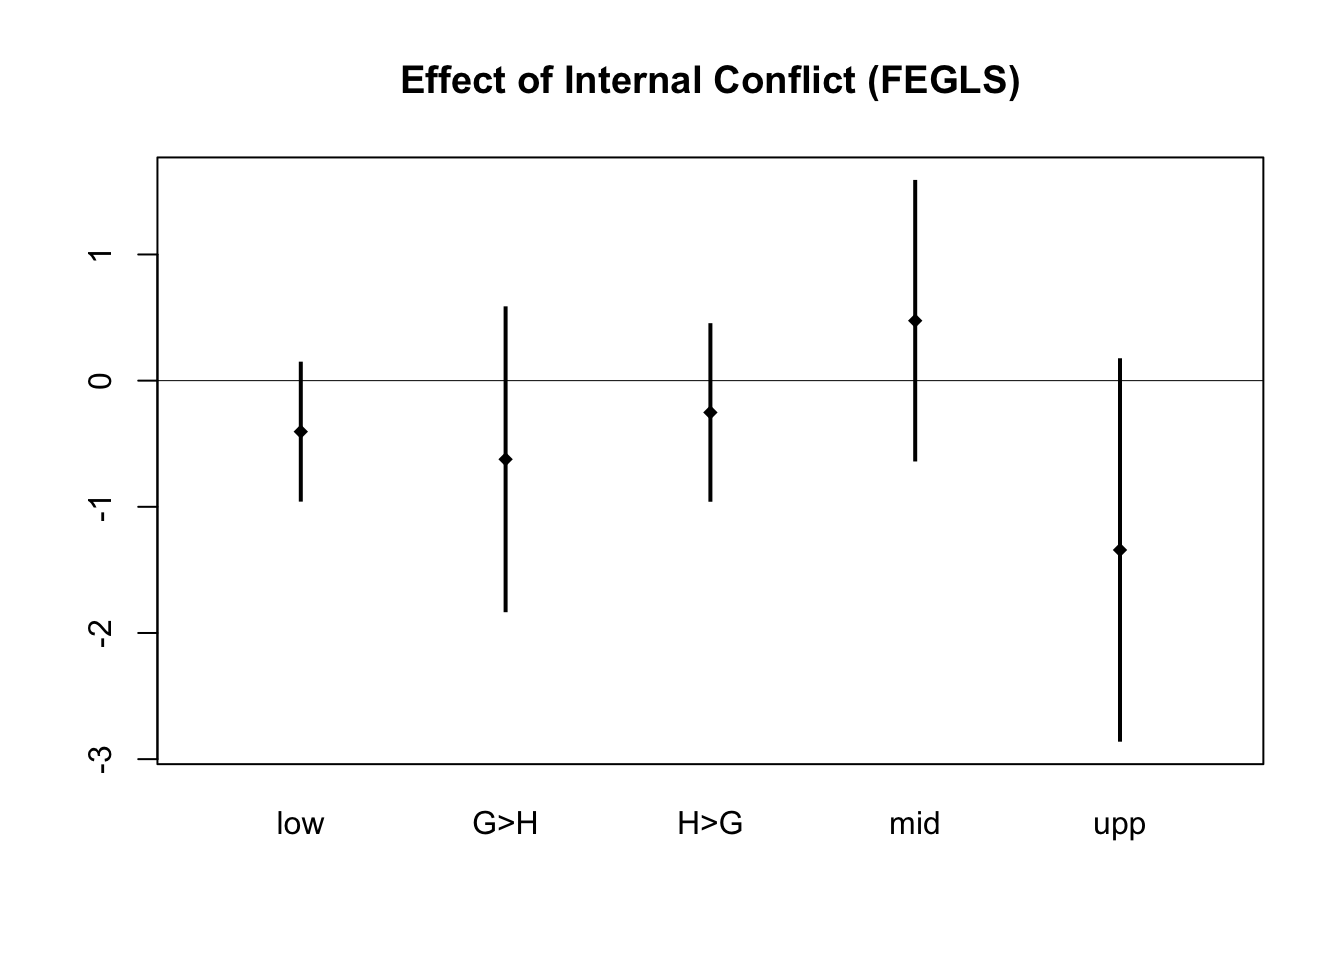
\includegraphics[width=0.67\textwidth]{figures/int_life_exp_conflict_incidence-4.png}
\end{figure}

\begin{figure}[!htb]
    \centering
    \caption{Effects of internal conflict deaths on life expectancy (with violence controls)}
    \label{int_life_exp_conflict_deaths}
    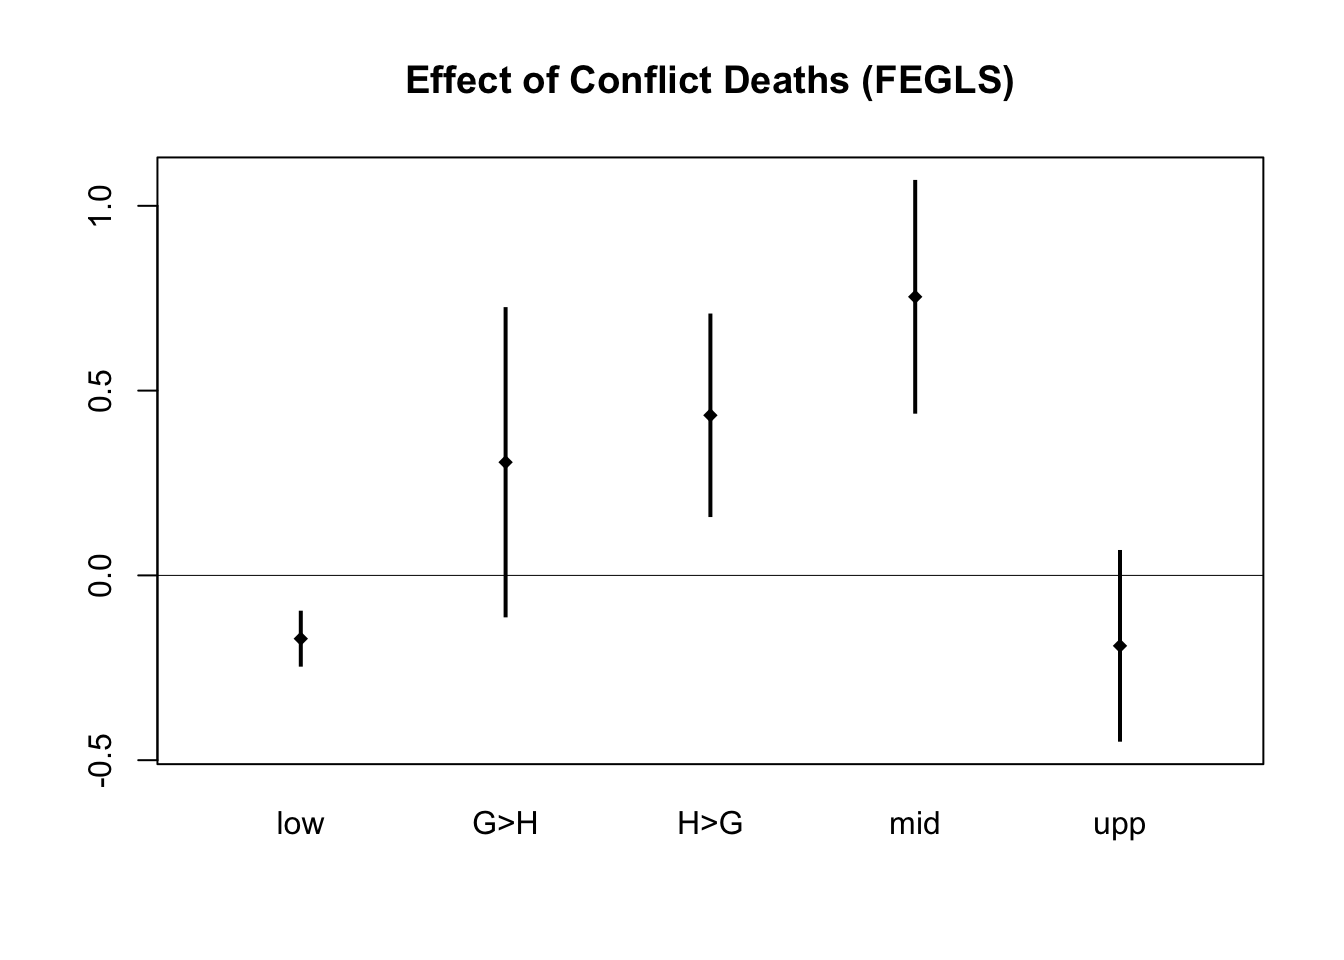
\includegraphics[width=0.67\textwidth]{figures/int_life_exp_conflict_deaths-4.png}
\end{figure}

The analyses of the IMR and UFMR outcome variables find support for a vicious cycle involving internal conflict.
The analyses of the IMR and UFMR outcome variables find similar support for a vicious cycle involving internal conflict deaths in the G>H classification.
Conflict incidence is associated with a worsening of the UFMR in the FEGLS model, and conflict deaths are associated with worsening of both IMR and UFMR in some models.
The interactions indicate that this effect is focused in the G>H classification, and less so in the low classification; \Cref{int_imr_conflict_deaths} shows an example.
The evidence for the UFMR is similar but weaker.
The results of the analyses of DALYs possibly contradict the notion of vicious cycles, since some of the internal conflict variables are associated with higher life expectancy, and these results are not robust across specifications.

\begin{figure}[!htb]
    \centering
    \caption{Effects of internal conflict deaths on IMR (with violence controls)}
    \label{int_imr_conflict_deaths}
    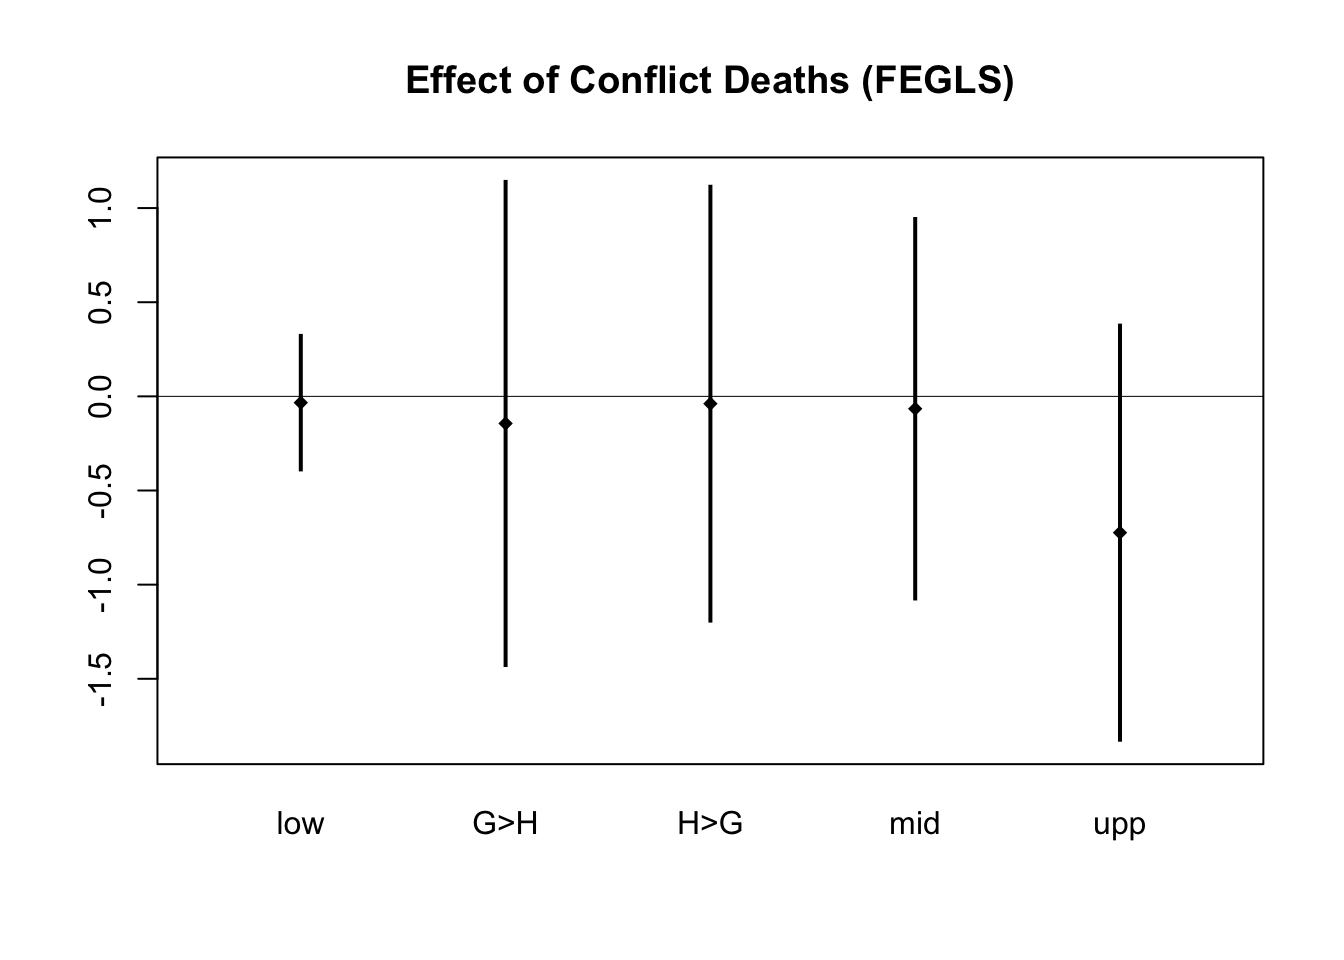
\includegraphics[width=0.67\textwidth]{figures/int_imr_conflict_deaths-4.png}
\end{figure}

The evidence is much more mixed with respect to the gender outcomes.
Some of the models of the MYS ratio seem to contradict the notion of vicious and virtuous cycles as conflict incidence is associated with higher ratios in lower classifications.
However, when other types of violence are controlled for, the evidence becomes weakly supportive, in that conflict incidence is associated with a decreased MYS ratio in the G>H classification or an increased ratio in the mid classification, depending on the estimator (not shown).
When substituting the conflict deaths measure, the situation is reversed. Without the controls for other types of violence, the results strongly support vicious and virtuous cycles, but when these controls are included, the results are very similar to those for conflict incidence, as shown in \Cref{int_mys_conflict_deaths}.

\begin{figure}[!htb]
    \centering
    \caption{Effects of internal conflict deaths on MYS ratio}
    \label{int_mys_conflict_deaths}
    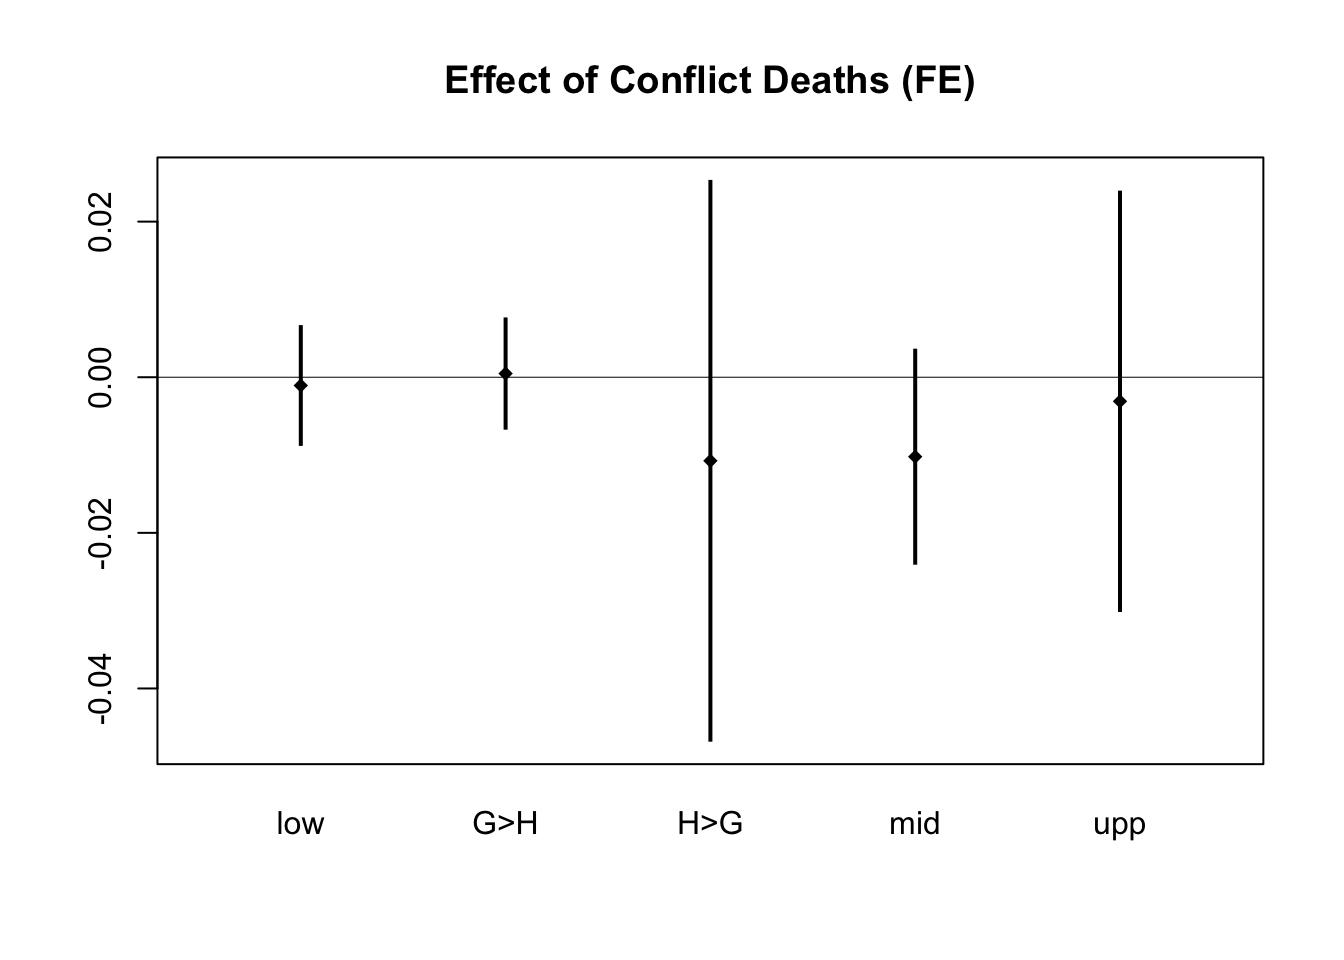
\includegraphics[width=0.45\textwidth]{figures/int_mys_conflict_deaths-3.png}
    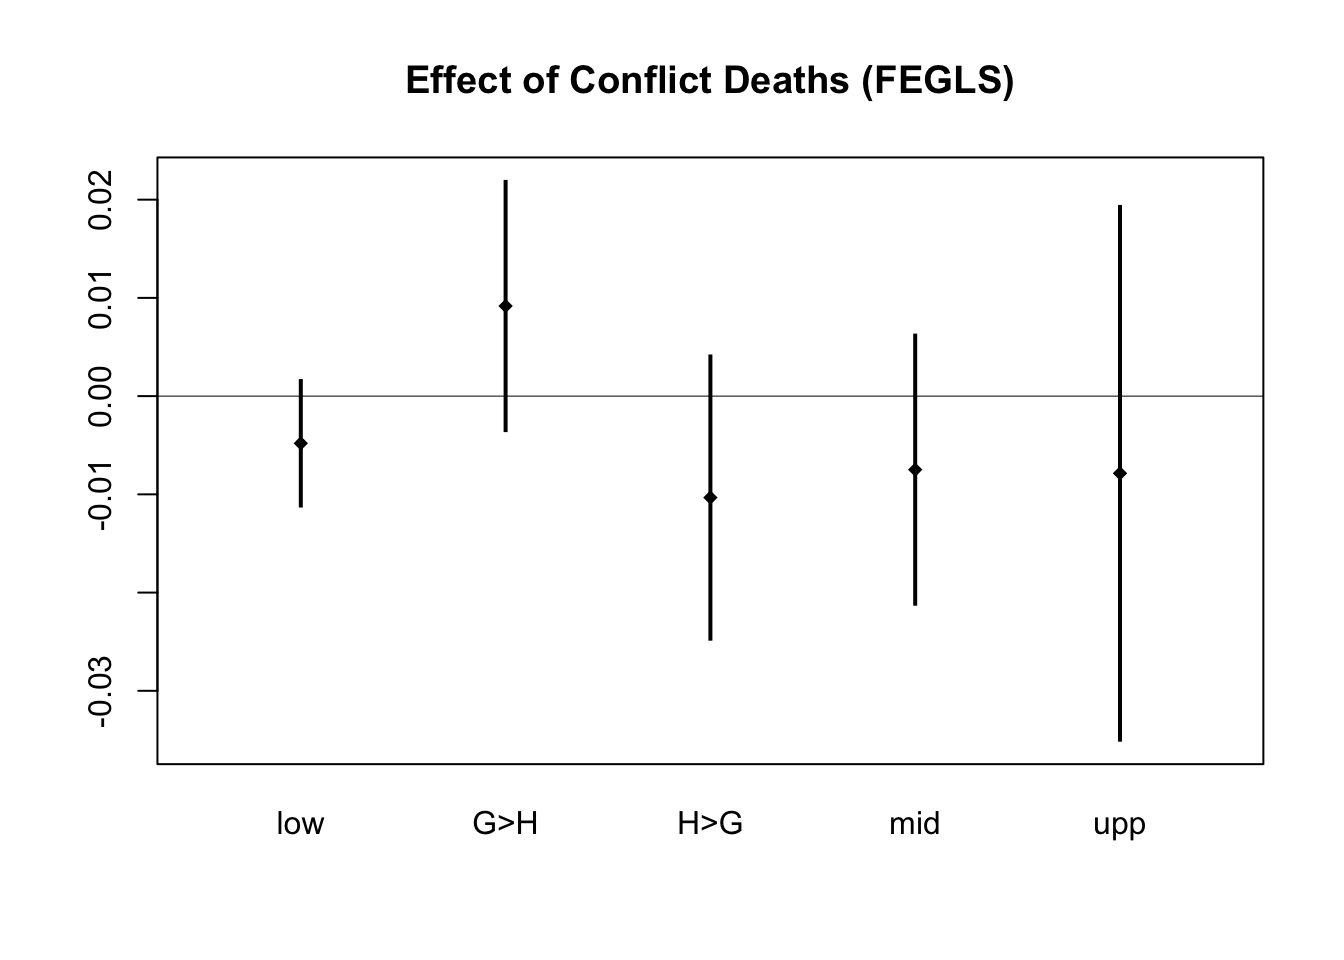
\includegraphics[width=0.45\textwidth]{figures/int_mys_conflict_deaths-4.png}
\end{figure}

The results of the AFR models are mixed and not robust.
\Cref{int_asfr_conflict} shows that both conflict incidence and deaths are associated with worse AFR in the G>H and upper classifications in the FEGLS models.
Finally, in the analyses of the Gender Inequality Index (GII), the conclusions depend on the choice of conflict variable. Conflict incidence is associated with a worsening GII in some models, particularly in the H>G classification (not shown).
However, \Cref{int_gii_conflict_deaths} lends limited support to a vicious cycle, as conflict deaths are associated with worse GII in the H>G and mid classifications in the FEGLS model, and these effects are statistically distinguishable from that in the lower and upper classifications, thus both supporting and contradicting the framework.

\begin{figure}[!htb]
    \centering
    \caption{Effects of internal conflict incidence and deaths on AFR (with violence controls)}
    \label{int_asfr_conflict}
    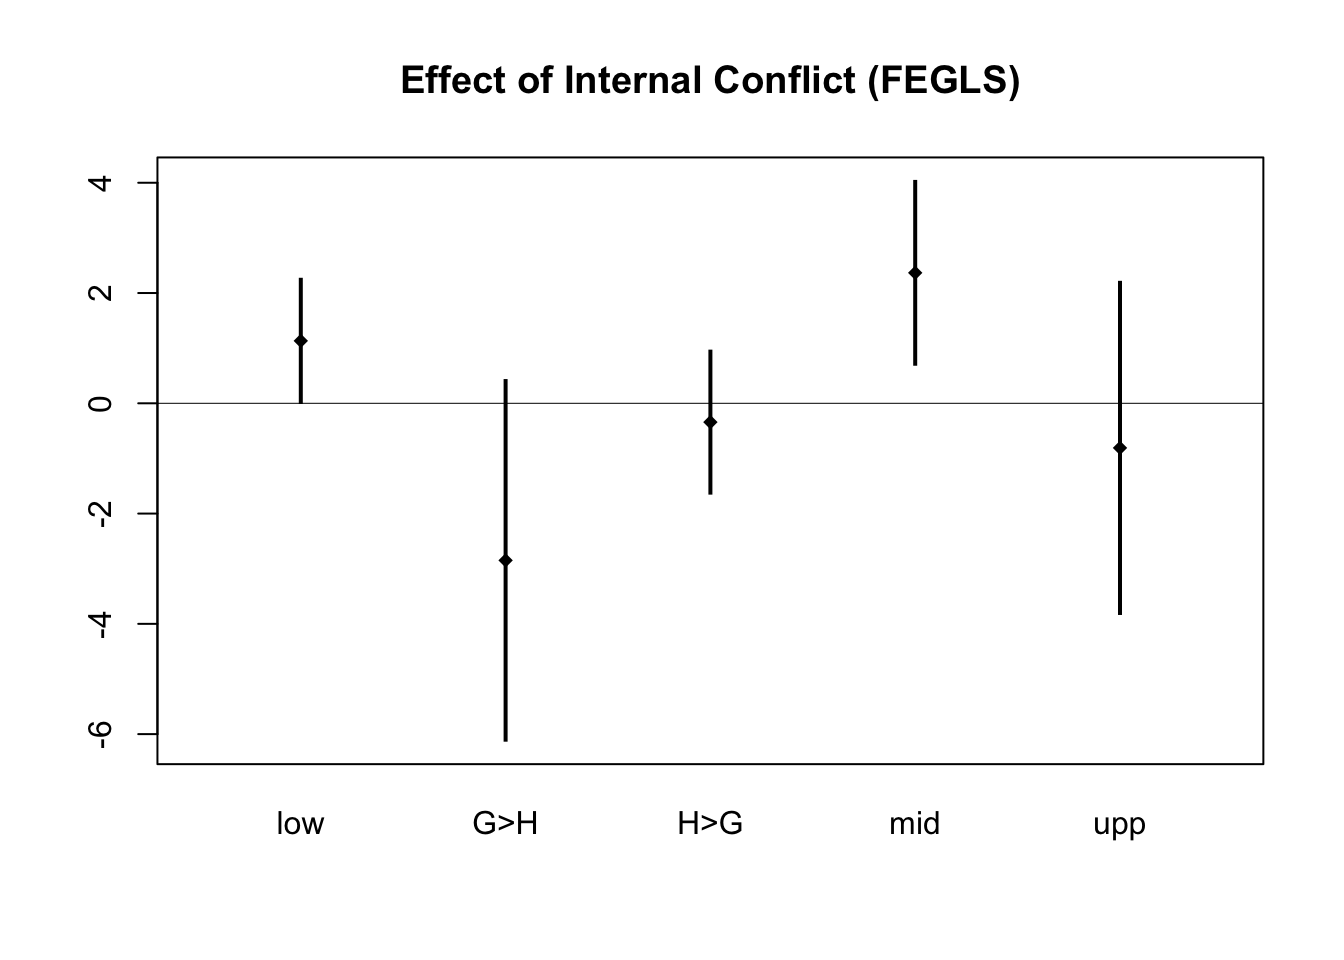
\includegraphics[width=0.45\textwidth]{figures/int_asfr_conflict_incidence-4.png}
    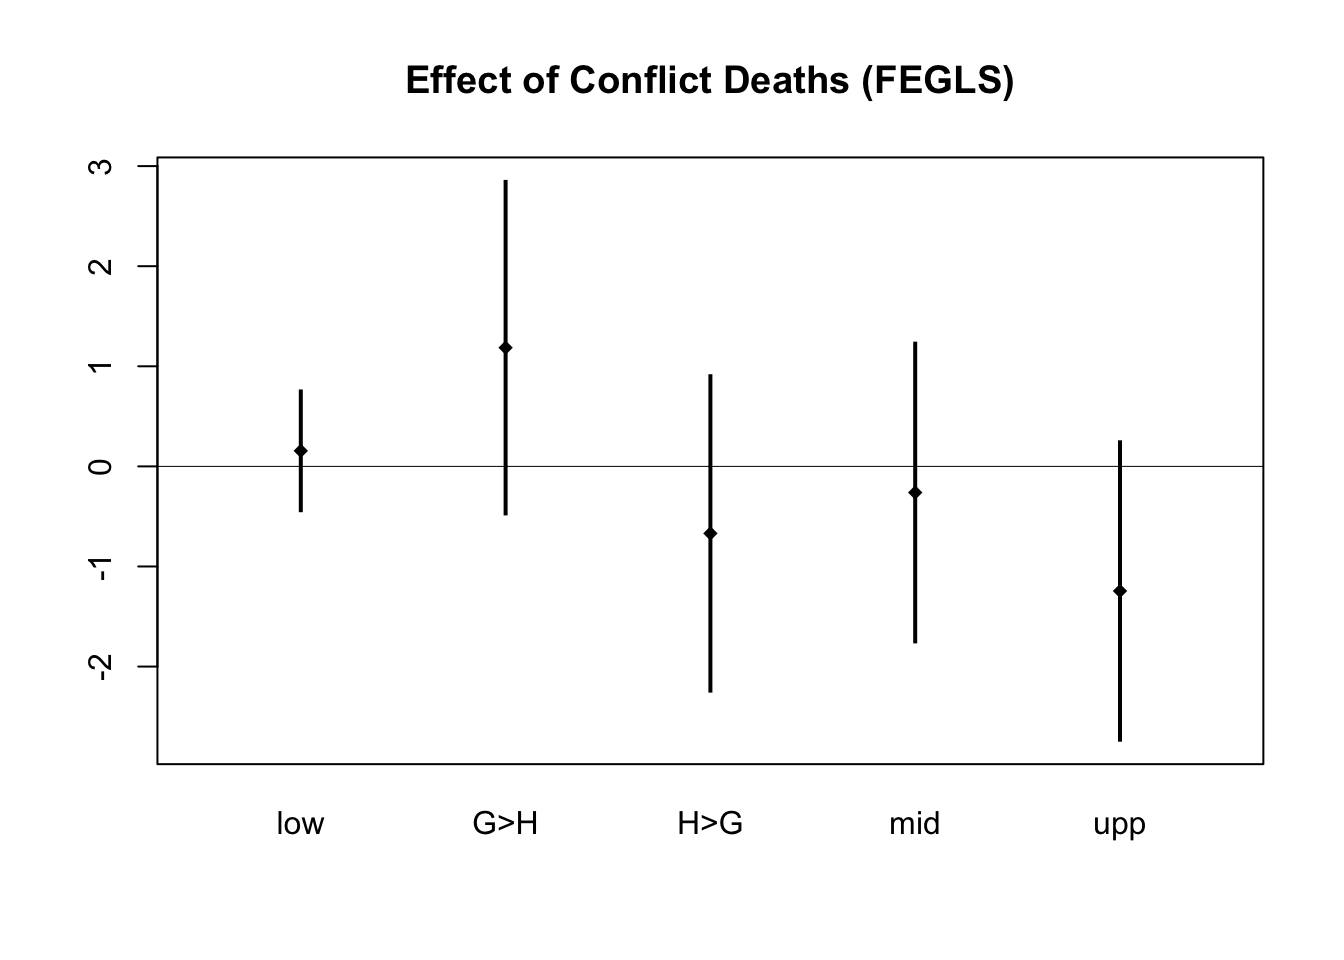
\includegraphics[width=0.45\textwidth]{figures/int_asfr_conflict_deaths-4.png}
\end{figure}

\begin{figure}[!htb]
    \centering
    \caption{Effects of internal conflict deaths on GII}
    \label{int_gii_conflict_deaths}
    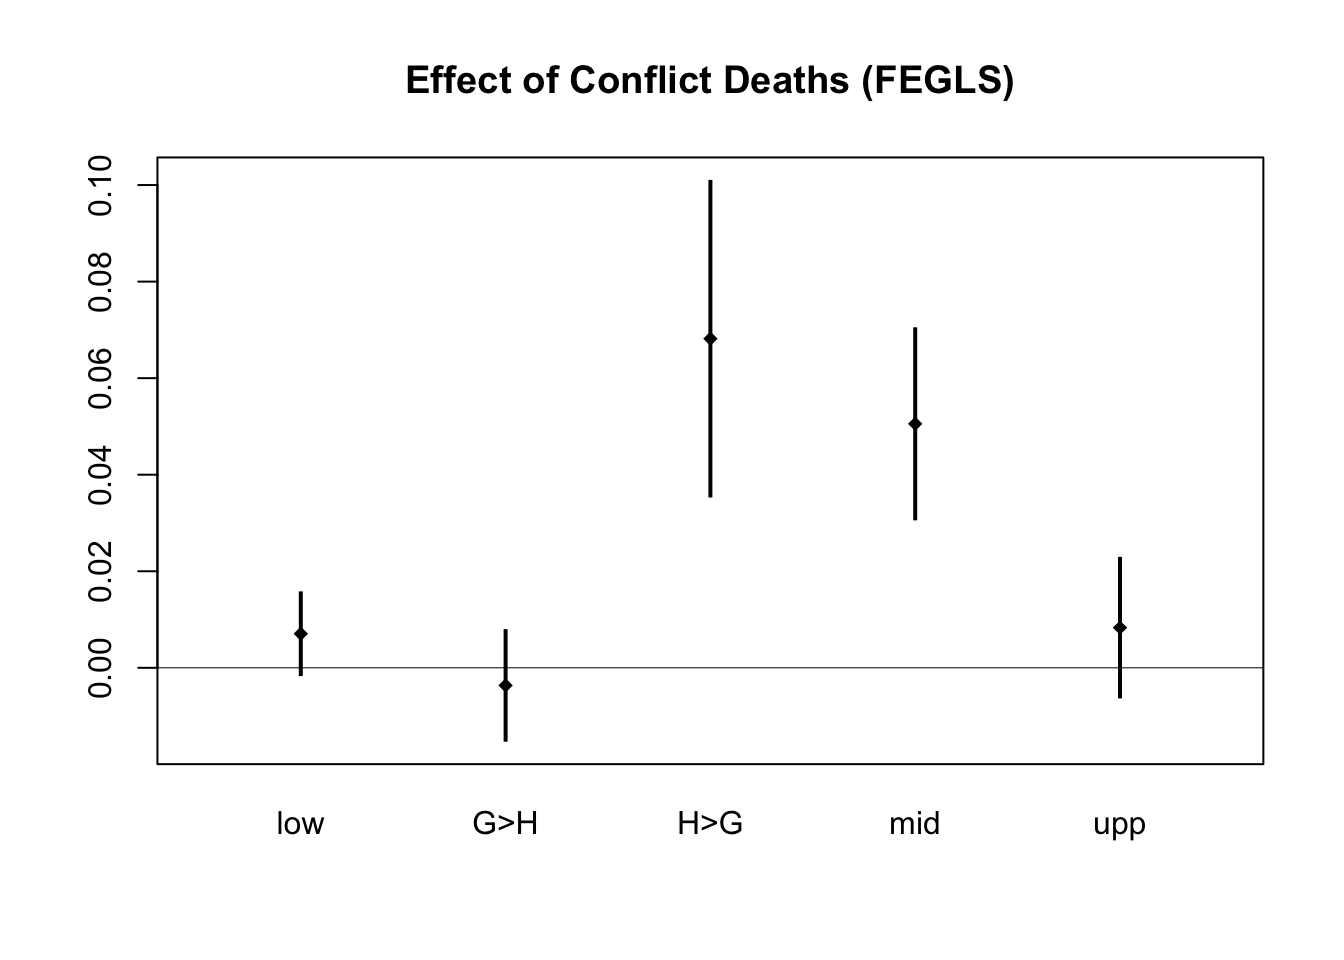
\includegraphics[width=0.67\textwidth]{figures/int_gii_conflict_deaths-4.png}
\end{figure}

Overall, the evidence for vicious and virtuous cycles involving internal conflict is weaker in the models of gender outcomes than for health outcomes.

\subsubsection{Statistical effects of state repression}

The analyses use four measures of violent state repression: UCDP's one-sided violence (OSV) incidence and deaths; the latent physical integrity (LPI) measure; and the V-Dem measure of extra-judicial killings.
One-sided violence incidence is associated with lower life expectancy in the low classification, and higher life expectancy in the H>G and mid classifications in \Cref{int_life_exp_osv_incidence}.
Unexpectedly, deaths due to OSV are actually associated with increases in life expectancy, including in the low classification in \Cref{int_life_exp_osv_deaths}.
The results are similar in models of the IMR or the UFMR, though not robust to the inclusion of the controls for other types of violence (not shown), with one exception.
One-sided violence deaths are associated with worse IMR and UFMR in the fixed effects models, particularly in the low, G>H and H>G classifications, which is consistent with a vicious cycle, but again, these results are not robust to accounting for other types of violence.
The models of DALYs do not support the proposed framework, and some even contradict it.

\begin{figure}[!htb]
    \centering
    \caption{Effects of OSV on life expectancy (with violence controls)}
    \label{int_life_exp_osv_incidence}
    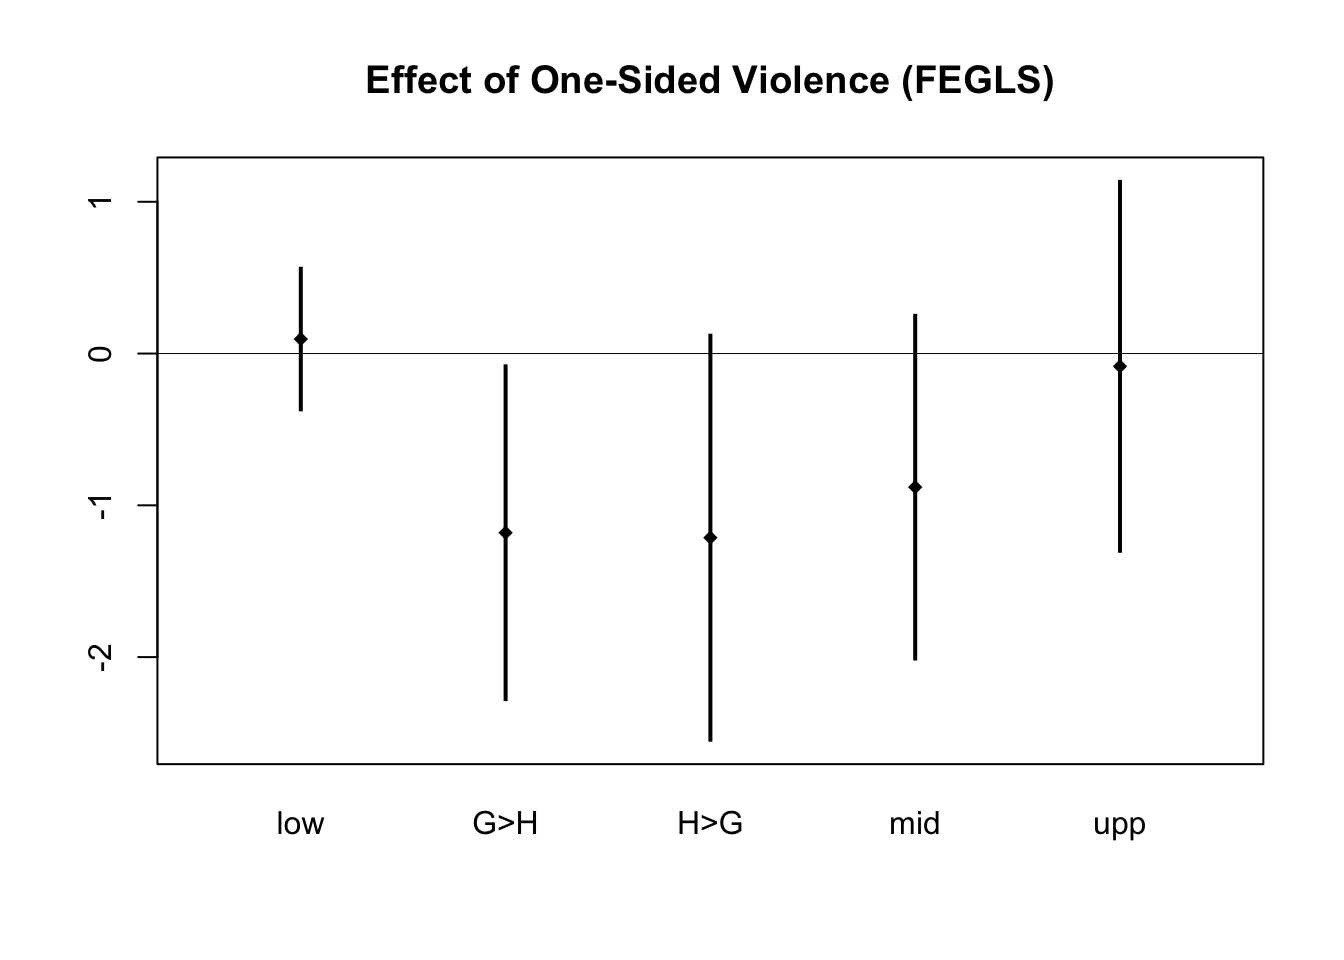
\includegraphics[width=0.67\textwidth]{figures/int_life_exp_osv_incidence-4.png}
\end{figure}
\begin{figure}[!htb]
    \centering
    \caption{Effects of OSV deaths on life expectancy}
    \label{int_life_exp_osv_deaths}
    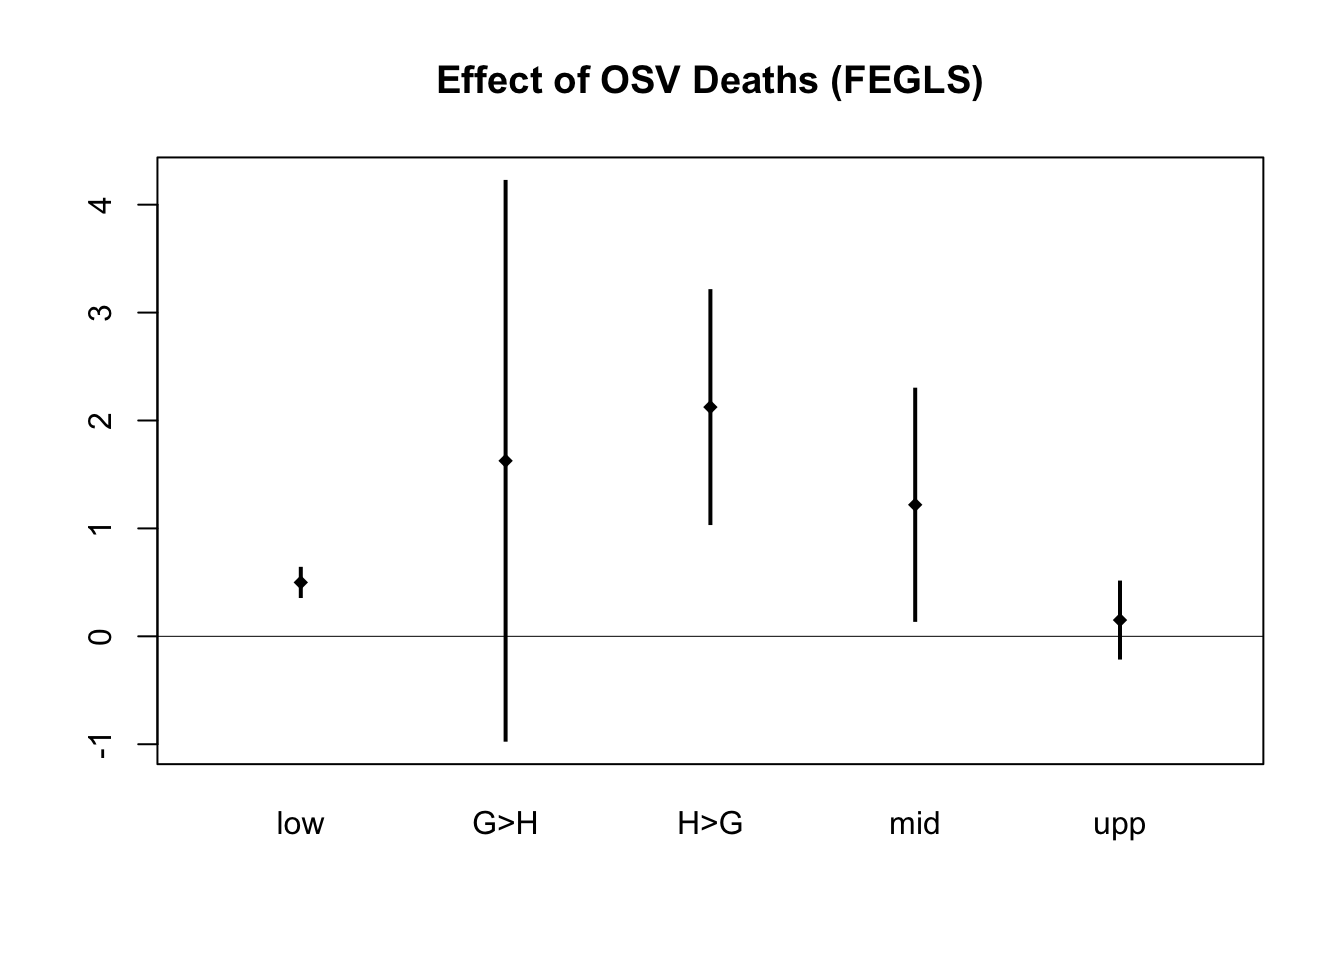
\includegraphics[width=0.67\textwidth]{figures/int_life_exp_osv_deaths-4.png}
\end{figure}
\begin{figure}[!htb]
    \centering
    \caption{Effects of OSV deaths on IMR}
    \label{int_imr_osv_deaths}
    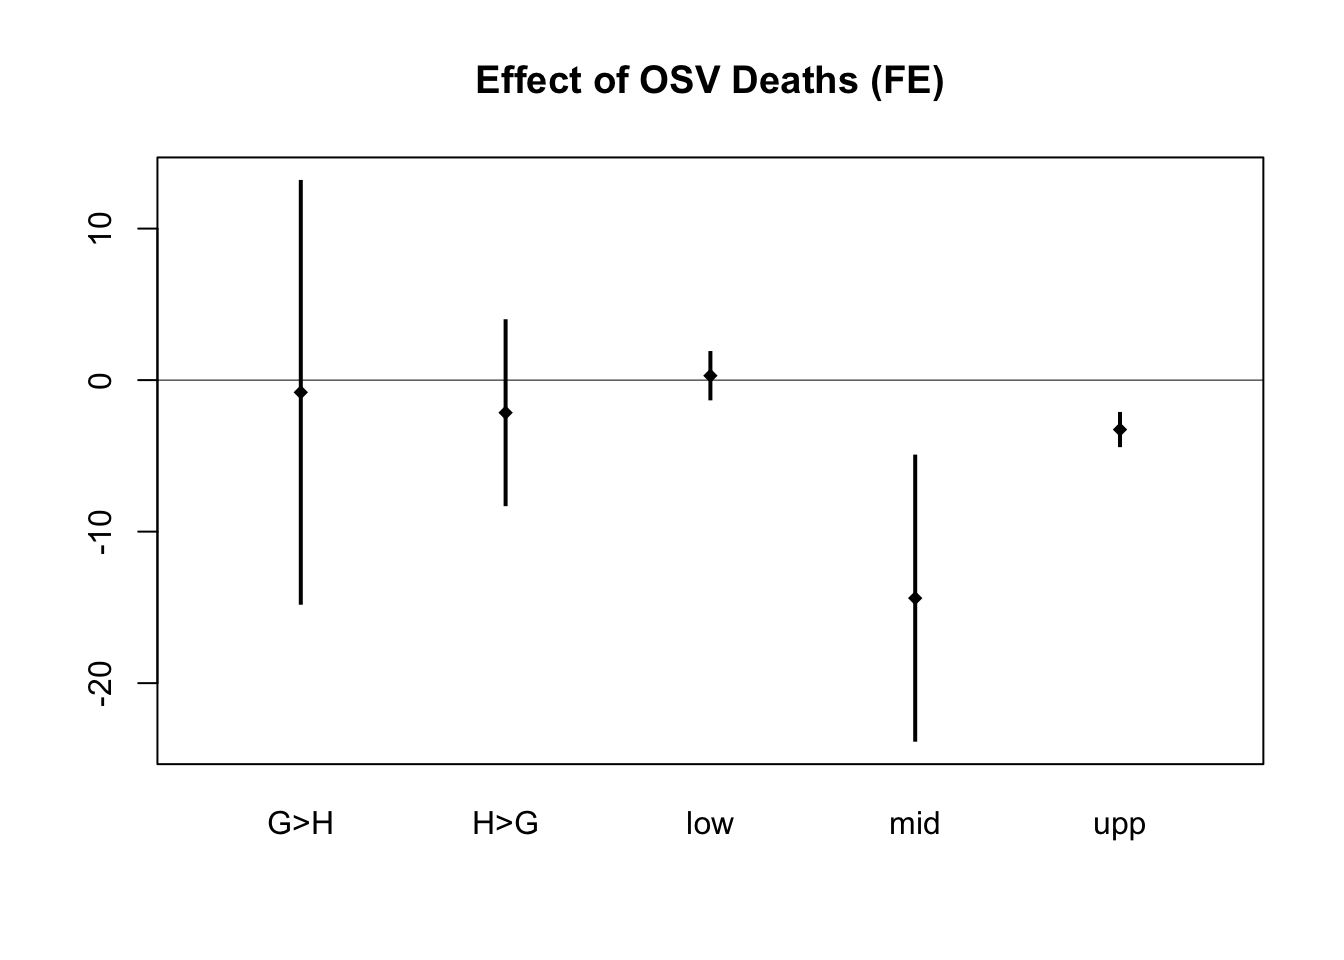
\includegraphics[width=0.67\textwidth]{figures/int_imr_osv_deaths-1.png}
\end{figure}

Similarly, evidence of vicious and virtuous cycles involving one-sided violence is quite limited in the models of gender outcomes. Both OSV incidence and deaths are associated with increases in the MYS ratio. In the case of incidence, this increase is strongly statistically significant in only the mid classification (not shown), but \Cref{int_mys_osv_deaths} provides mixed findings on OSV deaths, which are associated with increased MYS ratios in the low, H>G and mid classifications, but a decreased ratio in the G>H classification.
Furthermore, models of the AFR and the GII show few statistically significant effects and some contradictory effects.

\begin{figure}[!htb]
    \centering
    \caption{Effects of OSV deaths on MYS ratio}
    \label{int_mys_osv_deaths}
    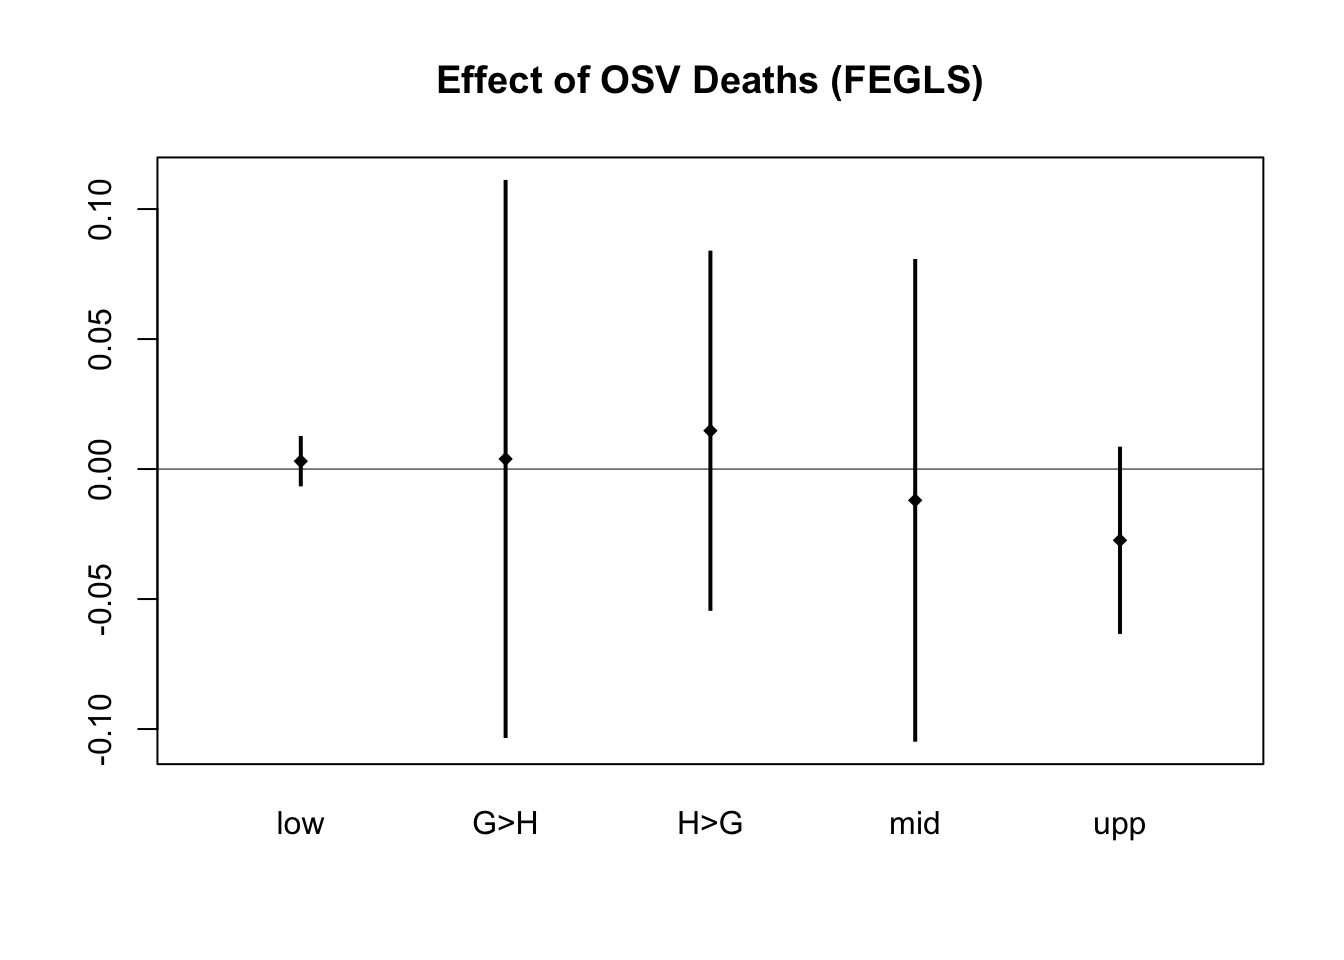
\includegraphics[width=0.67\textwidth]{figures/int_mys_osv_deaths-4.png}
\end{figure}

The other measures of violent state repression are conceptually related but often lead to different conclusions.
The measure of latent physical integrity, which covers a range of violations, is associated with increases in life expectancy in some models, but these are not distinguished much between classification groups.
This finding does not support vicious or virtuous cycles.
Unsurprisingly, extra-judicial killings, are strongly associated with decreased life expectancy, but only in the low classification in \Cref{int_life_exp_killings} and statistically distinguishable from the H>G, mid and upper classifications.
This finding strongly suggests a vicious cycle.

\begin{figure}[!htb]
    \centering
    \caption{Effects of extra-judicial killings on life expectancy (with violence controls)}
    \label{int_life_exp_killings}
    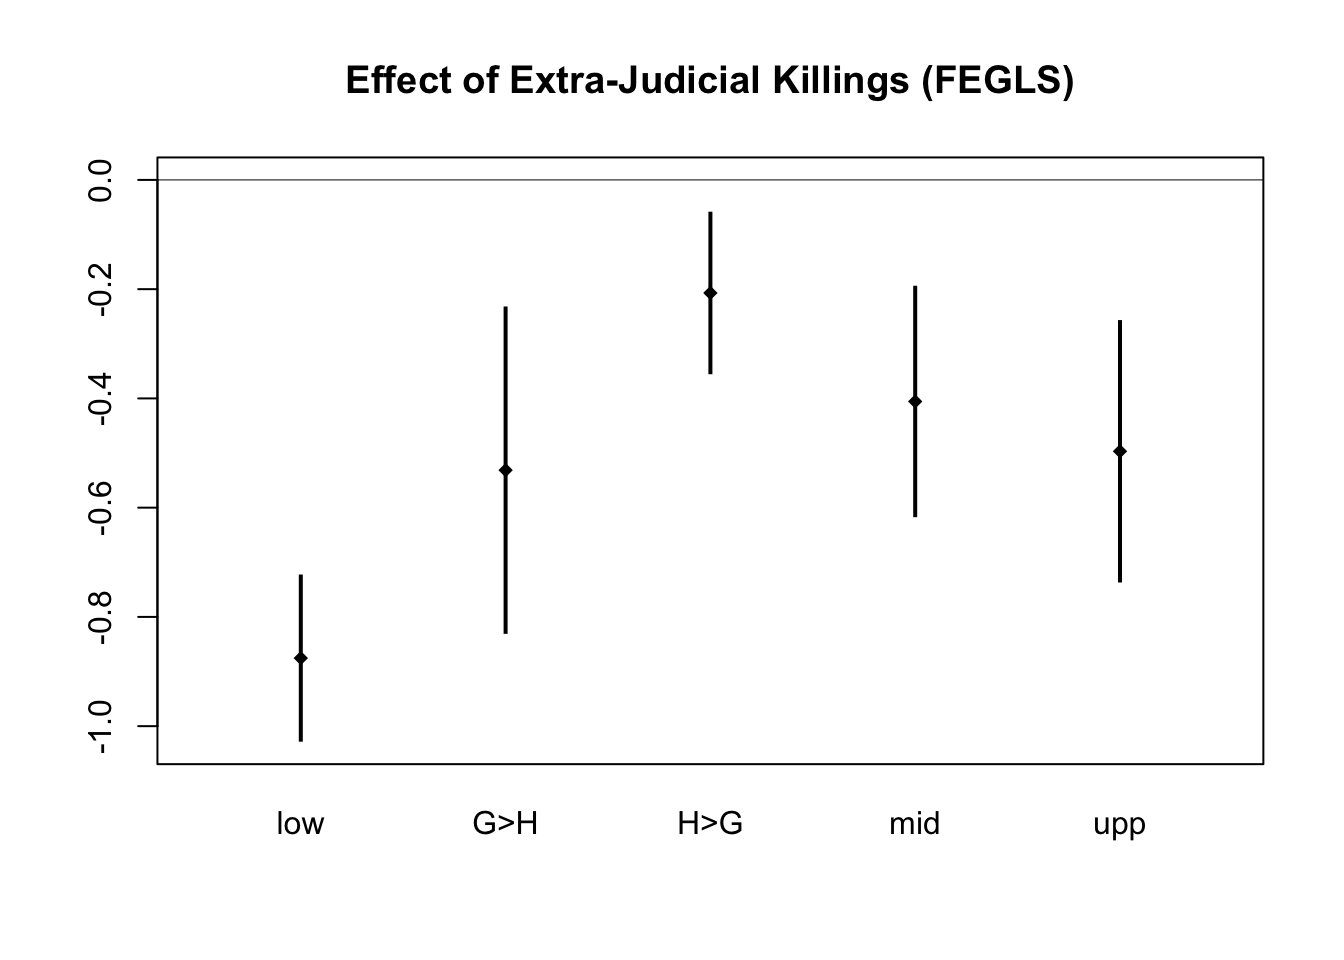
\includegraphics[width=0.67\textwidth]{figures/int_life_exp_killings-4.png}
\end{figure}

The LPI is associated with improvements in the IMR in the H>G, mid, and upper classifications in \Cref{int_imr_lpi}.
This suggests that violence only curtails improvements in the low and G>H classifications, but these results are sensitive to both the estimator used and whether other types of violence are accounted for.
The results for the UFMR are similar and stronger (not shown).
When substituting the measure of extra-judicial killings, the results for the IMR and the UFMR are similar to those for life expectancy in \Cref{int_life_exp_killings}, but these results are sensitive to model specification.
Models of DALYs also provide similarly supportive evidence for vicious and virtuous cycles (not shown).

\begin{figure}[!htb]
    \centering
    \caption{Effects of physical integrity violations on IMR (with violence controls)}
    \label{int_imr_lpi}
    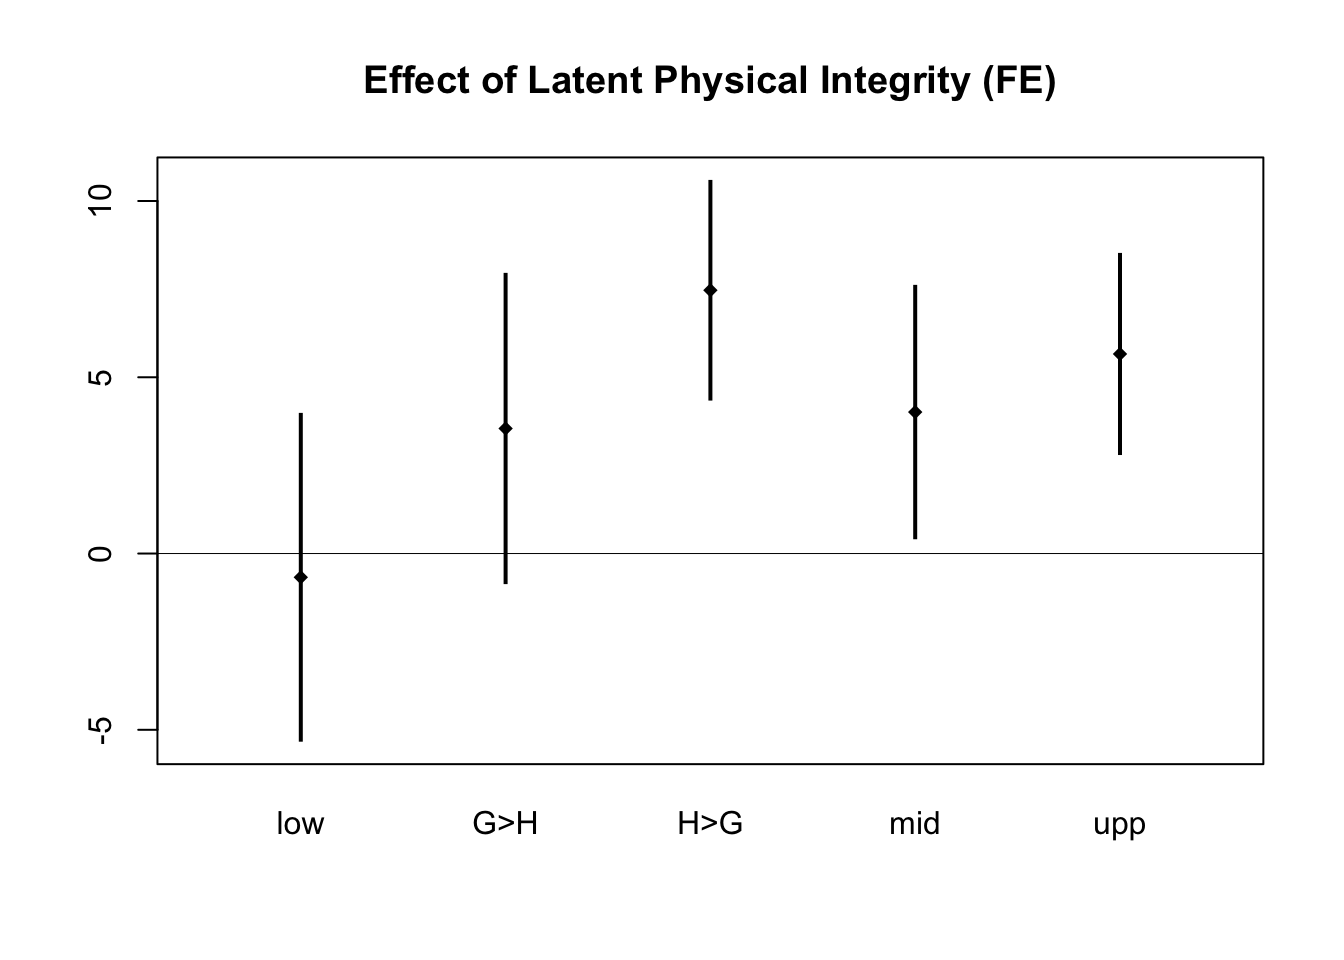
\includegraphics[width=0.67\textwidth]{figures/int_imr_lpi-3.png}
\end{figure}

With respect to gender outcomes, the models of the MYS ratio and of the AFR, the findings are mixed, providing evidence for and against the proposed framework.
The LPI measure is associated with higher MYS ratios in the low, mid, and upper classifications in the FEGLS model in \Cref{int_mys_lpi}, but a decreased ratio in the G>H classification.
In \Cref{int_asfr_lpi}, the LPI has similar effects on changes in the AFR, which are strongly statistically significant, but these are not robust to accounting for other types of violence.
These figures show associations in the low classification that contradict vicious cycles but otherwise provide support for vicious and virtuous cycles in other classifications.
Substituting the V-Dem measure of extra-judicial killings provides similarly supportive but weak evidence that is not robust to different model specifications.
Finally, models of the Gender Inequality Index provide some evidence that latent physical integrity violations and extra-judicial killings are associated with improvements only in the middle classifications (not shown).

\begin{figure}[!htb]
    \centering
    \caption{Effects of physical integrity violations on MYS ratio (with violence controls)}
    \label{int_mys_lpi}
    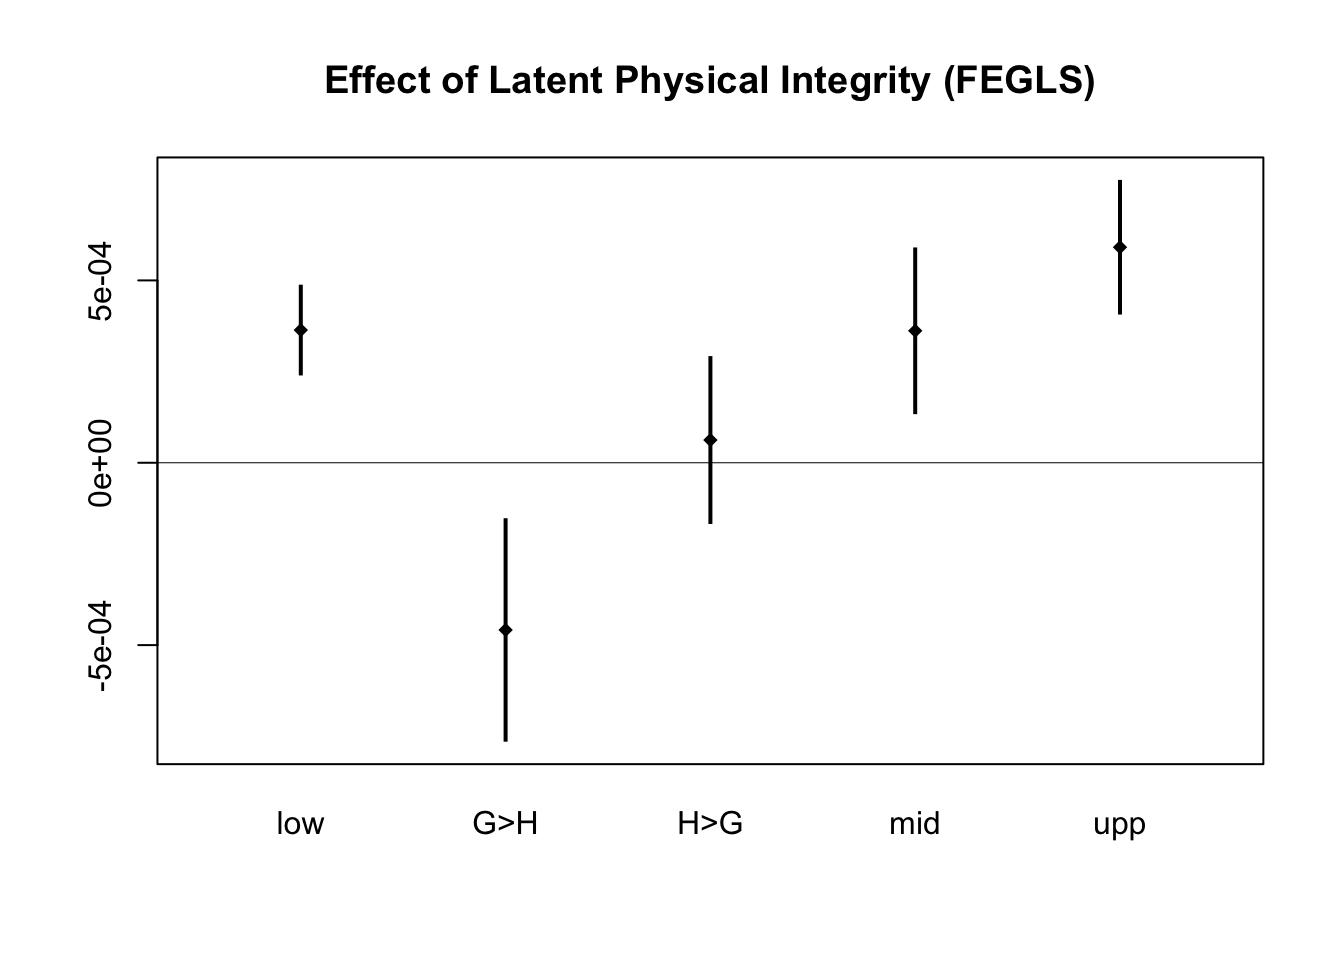
\includegraphics[width=0.67\textwidth]{figures/int_mys_lpi-4.png}
\end{figure}
\begin{figure}[!htb]
    \centering
    \caption{Effects of physical integrity violations on AFR}
    \label{int_asfr_lpi}
    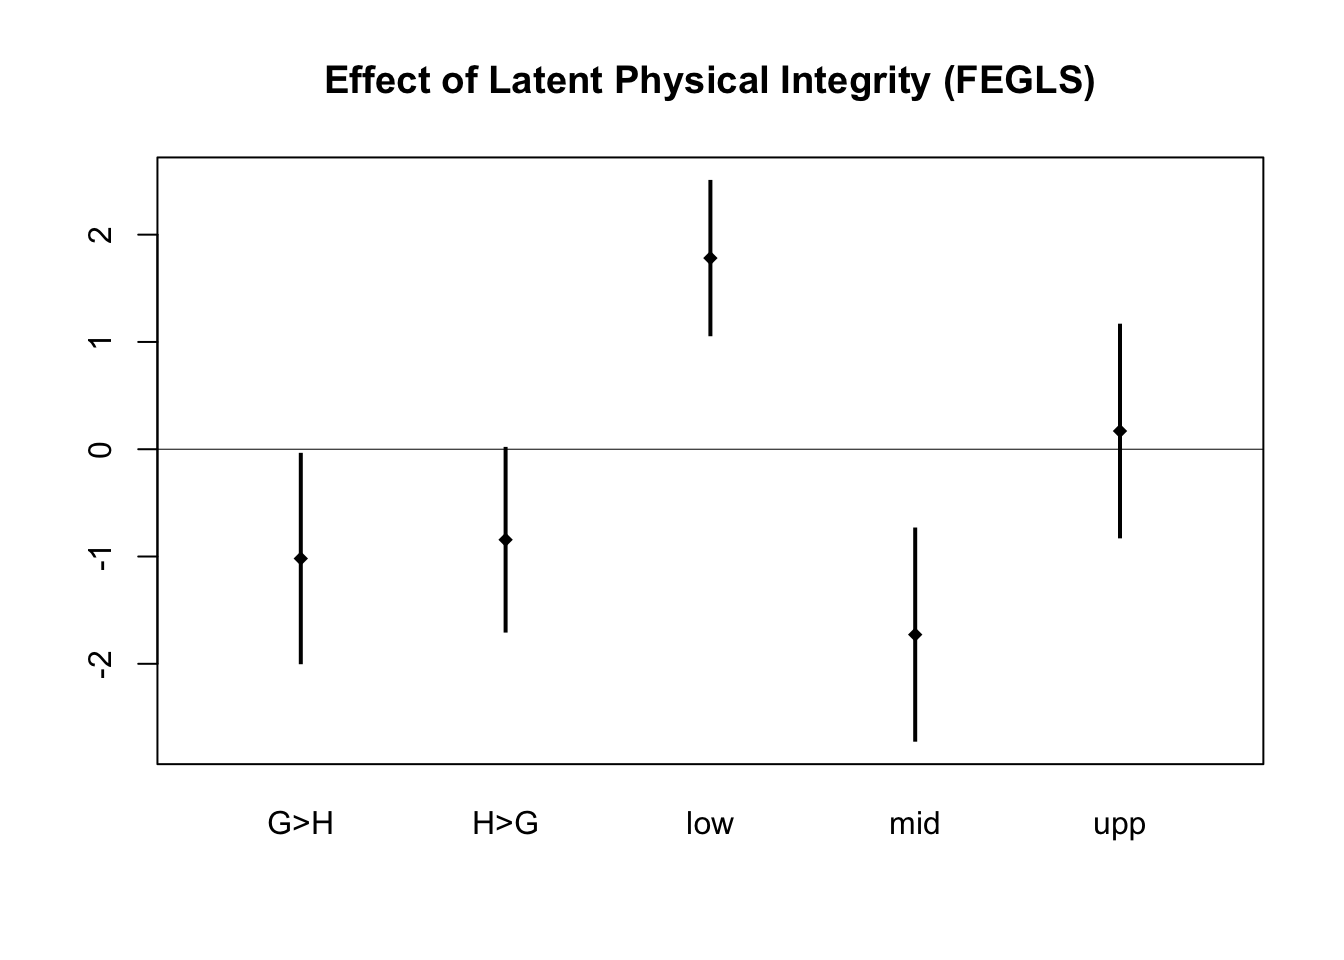
\includegraphics[width=0.67\textwidth]{figures/int_asfr_lpi-2.png}
\end{figure}

% % killings MYS: up in FEGLS
% \begin{figure}[!htb]
%     \centering
%     \caption{Effects of extra-judicial killings on MYS ratio}
%     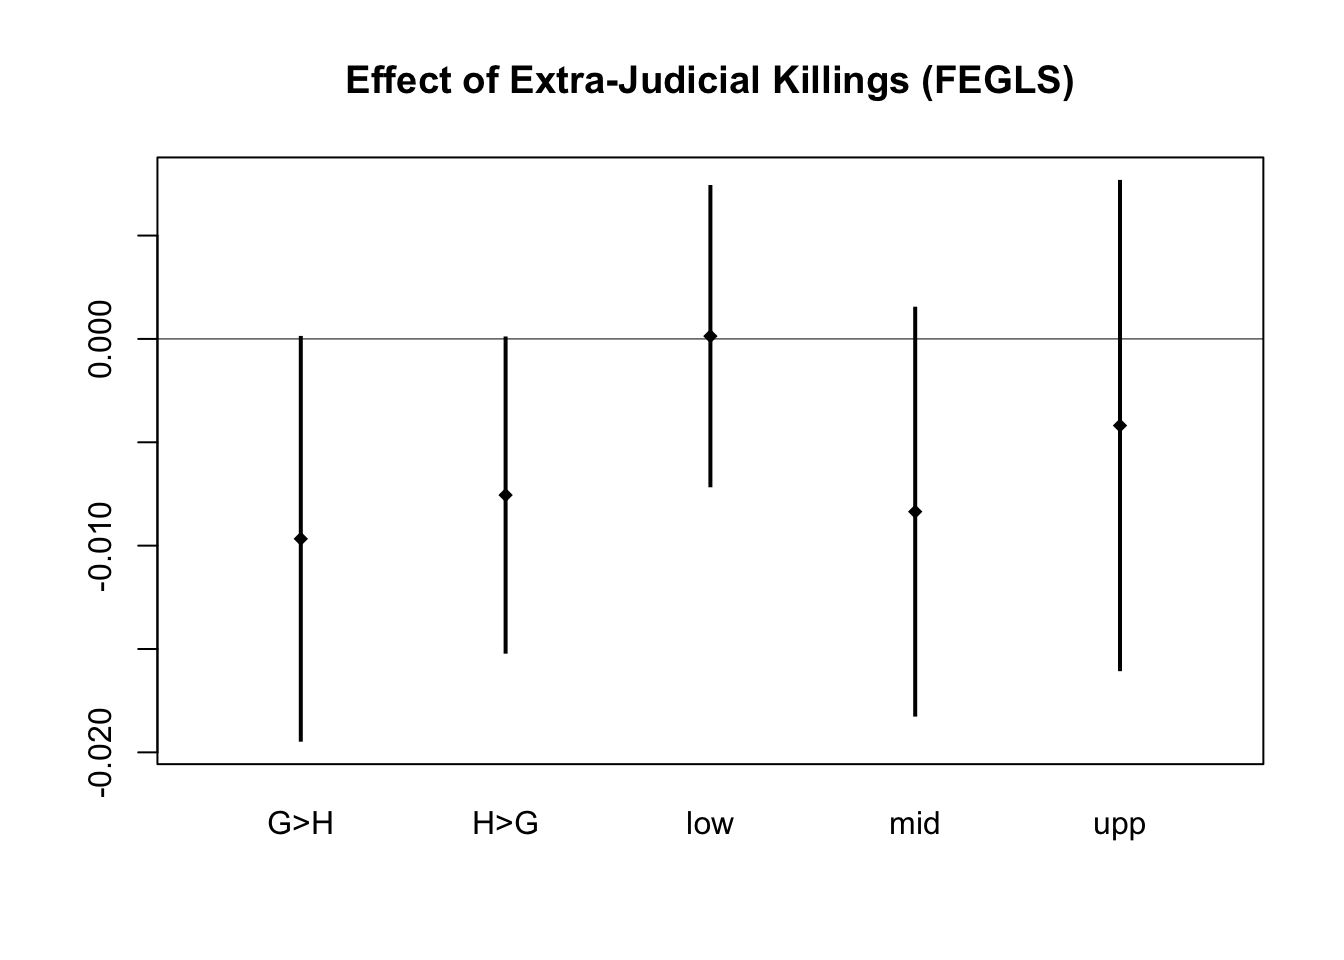
\includegraphics[width=0.45\textwidth]{figures/int_mys_killings-2.png}
%     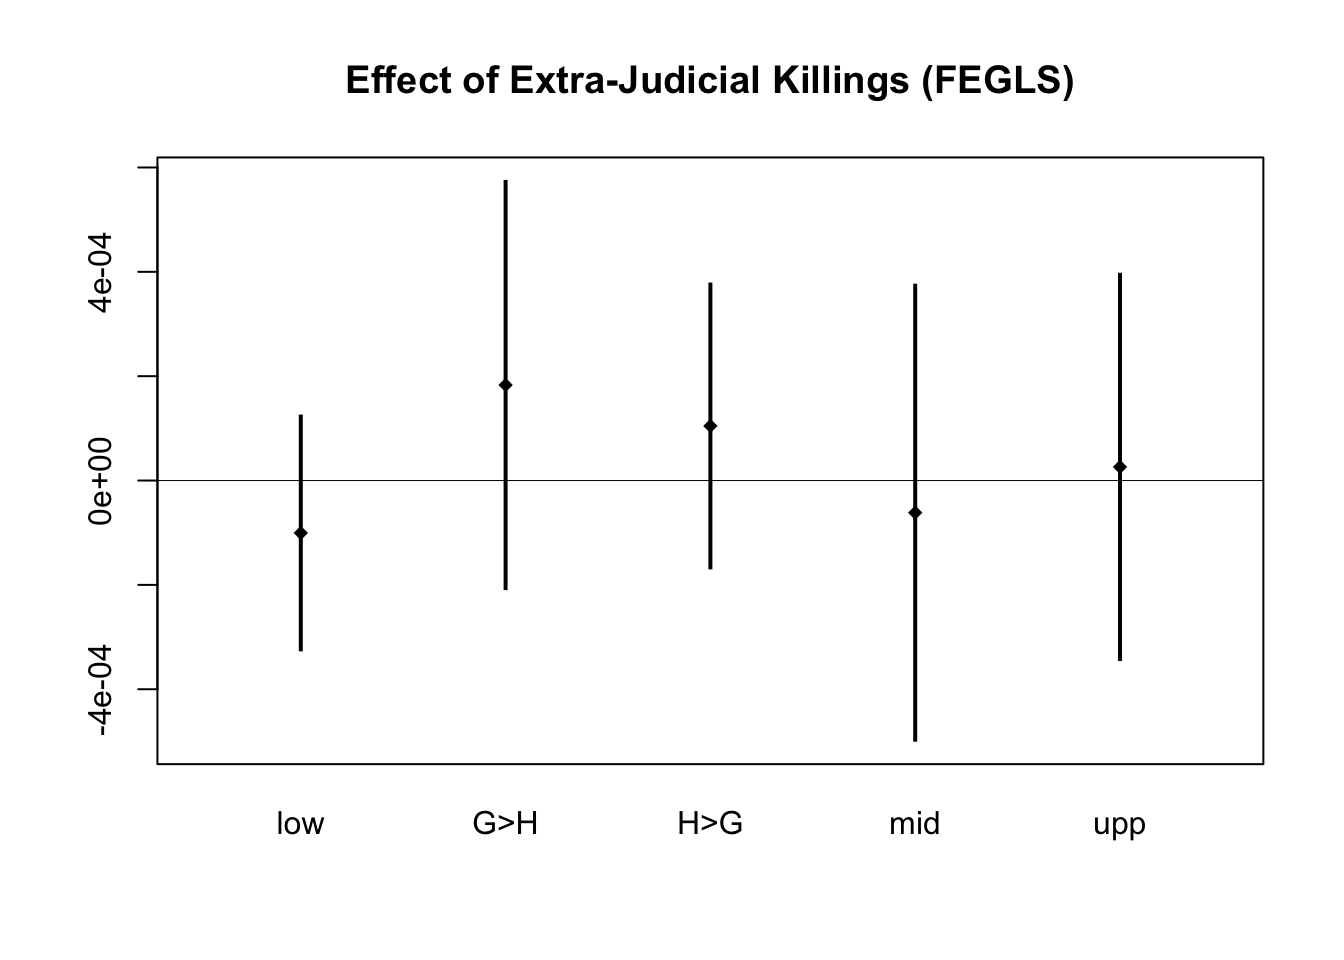
\includegraphics[width=0.45\textwidth]{figures/int_mys_killings-4.png}
% \end{figure}

% % killings AFR: down in FEGLS
% \begin{figure}[!htb]
%     \centering
%     \caption{Effects of extra-judicial killings on AFR}
%     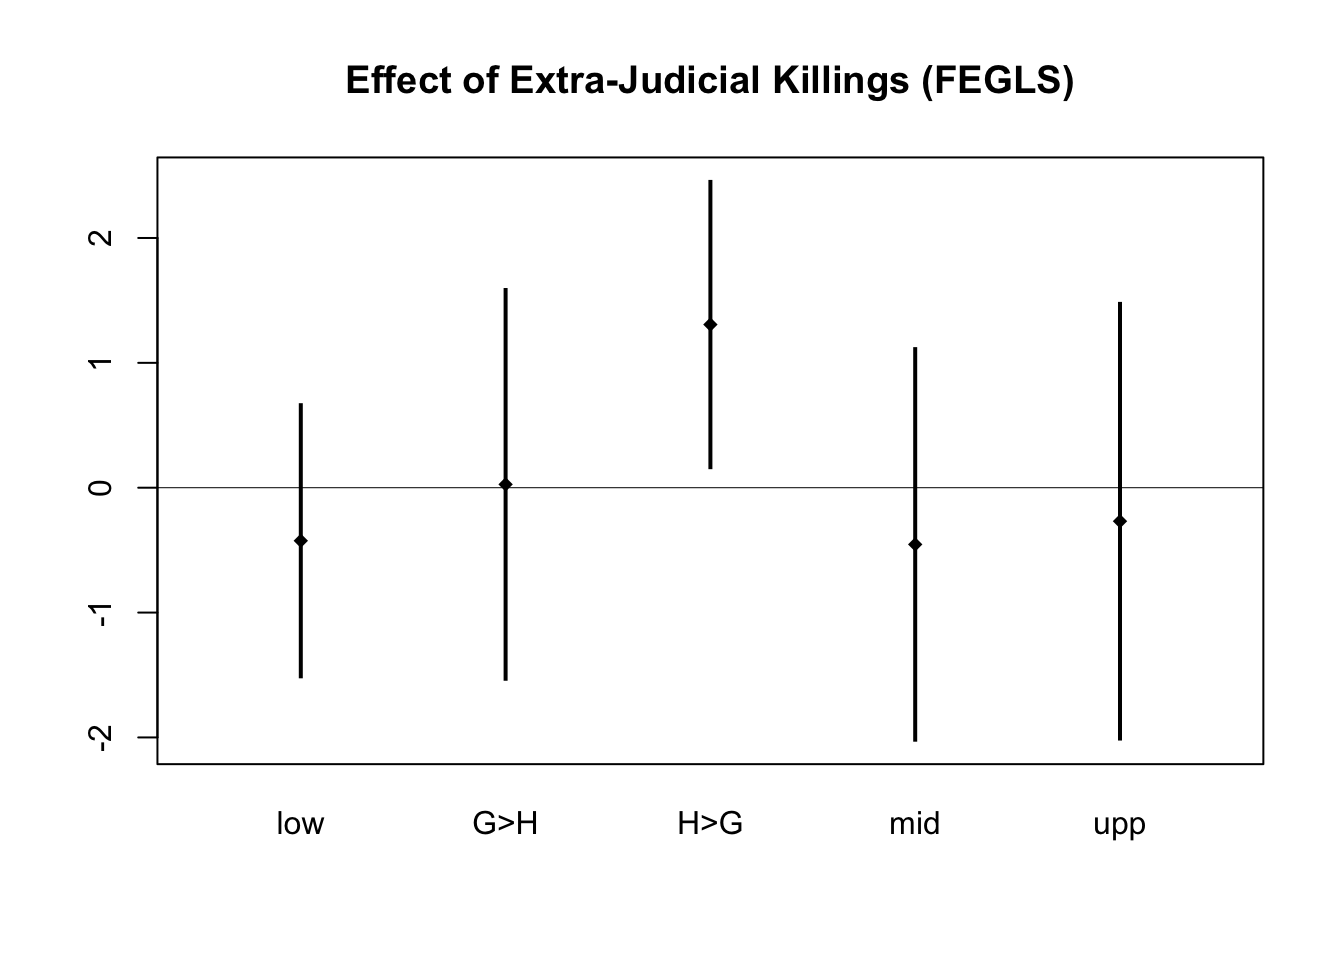
\includegraphics[width=0.67\textwidth]{figures/int_asfr_killings-2.png}
% \end{figure}

\clearpage
\begin{sidewaystable}[!htbp]
\small
\centering
\caption{Summary of findings on health and gender outcomes: repression interactions}
\label{table_hg_repression}
\begin{tabular}{lccccccccccc}
\toprule
                                     & Life         & IMR          & UFMR         & DALYs     & MYS                      & AFR                  & Labor part. & GII \\
                                     & Expectancy   &              &              &           & ratio                    &                      & ratio       & \\
\midrule
one-sided violence incidence         &              &              &              &           & $+$ \ddag                &                      &             & \\
--- low classification interaction   & $-$ \ddag    & $-$ \dag\ *  & $-$ \dag\ *  &           &                          & $+$ \ddag            &             & \\
--- G$>$H classification interaction & $-$ *        &              &              &           &                          &                      &             & \\
--- H$>$G classification interaction & $+$ \ddag    & $+$ \ddag    &              &           & $+$ \ddag\ *             &                      &             & $+$ \\
--- mid classification interaction   & $+$ \ddag    & $+$ \ddag\ * &              &           & $+$ \ddag                &                      &             & $-$ \dag\ * \\
--- upp classification interaction   & $+$ \ddag\ * &              &              &           &                          & $-$ \ddag            &             & \\
\midrule
one-sided violence deaths            & $+$          & $-$ \dag     & $-$ \dag     & $+$ \ddag & $+$ \ddag                &                      &             & \\
--- low classification interaction   & $+$          & $-$ \dag     & $-$ \dag     & $+$ \ddag & $+$ \dag                 &                      & $+$ \dag    & \\
--- G$>$H classification interaction & $-$ \dag\ *  & $-$ \dag\ *  &              & $+$ \dag  & $-$ \ddag                &                      &             & \\
--- H$>$G classification interaction & $+$ \ddag    & $-$ \dag\ *  & $-$ \dag\ *  &           & $+$ \ddag                & $-$ \dag             & $-$ \dag    & $+$ \ddag \\
--- mid classification interaction   &              &              &              & $+$ \ddag & $+$ \ddag                &                      &             & \\
--- upp classification interaction   &              &              &              &           &                          &                      &             & \\
\midrule
state repression (LPI)               & $+$ \ddag    &              & $+$ \dag     &           & $+$ \ddag                & $+$                  &             & \\
--- low classification interaction   &              & $-$ \ddag\ * & $-$ \ddag\ * & $-$ \ddag & $+$ \ddag                & $+$ *                &             & \\
--- G$>$H classification interaction &              &              & $+$ \dag     & $+$ \dag  & $-$                      & $-$ \ddag\ *         &             & \\
--- H$>$G classification interaction & $+$ \dag\ *  & $+$ *        & $+$ *        & $+$ \dag  & $-$ \ddag\ *             & $+$ \ddag\ *         &             & $+$ \ddag \\
--- mid classification interaction   & $+$ \dag     & $+$ \dag     & $+$ \dag     & $+$ \dag  & $+$ \ddag                &                      &             & $+$ \ddag \\
--- upp classification interaction   &              & $+$ *        & $+$ *        & $+$ \dag  & $+$                      & $+$ \dag\ / \ddag\ * &             & \\
\midrule
extra-judicial killings              &              &              & $-$ \ddag    & $-$ \ddag & $+$ \ddag                & $-$ \ddag            &             & $+$ \ddag \\
--- low classification interaction   & $-$ \ddag    & $-$ *        & $-$ *        & $-$ \ddag & $+$ \ddag\ *             & $-$ \ddag\ *         &             & \\
--- G$>$H classification interaction &              &              &              & $+$ \dag  & $-$ \ddag\ *             & $-$ \ddag\ *         &             & $+$ \ddag \\
--- H$>$G classification interaction & $+$ \dag\ *  &              & $+$ \dag     & $+$ \dag  & $-$ \ddag\ * / $+$ \ddag &                      &             & $+$ \ddag \\
--- mid classification interaction   & $+$ \dag     &              & $+$ \dag     & $+$ \dag  & $-$ \ddag\ * / $+$ \ddag & $+$ \dag\ *          &             & $+$ \ddag \\
--- upp classification interaction   &              & $+$ \dag     & $+$ \dag     & $+$ \dag  & $+$ \ddag\ *             &                      &             & \\
\bottomrule
\end{tabular}
\caption*{\footnotesize Legend:
$+$, $-$ statistically significant effects;
\dag\ FE model only;
\ddag\ FEGLS model only;
* model does not include controls for other types of violence.}
\end{sidewaystable}

\clearpage

\subsubsection{Statistical effects of non-state conflict}

Non-state conflict is organized violence between societal actors, measured by two variables, incidence and battle-related deaths.
In FEGLS models, both non-state conflict incidence and deaths are associated with decreases in life expectancy, and the FE model in \Cref{int_life_exp_nsc_incidence} suggests a vicious cycle in the G>H classification group and a virtuous cycle in the mid classification, but these results are not robust to the choice of estimator. In the FEGLS models, non-state conflict is associated with a decrease in life expectancy in the lowest and highest classifications.
Substituting the non-state conflict death rate in the FE model leads to more support for vicious and virtuous cycles, as shown in \Cref{int_life_exp_nsc_deaths}, but again not in the FEGLS model (not shown).

\begin{figure}[!htb]
    \centering
    \caption{Effect of non-state conflict on life expectancy (with violence controls)}
    \label{int_life_exp_nsc_incidence}
    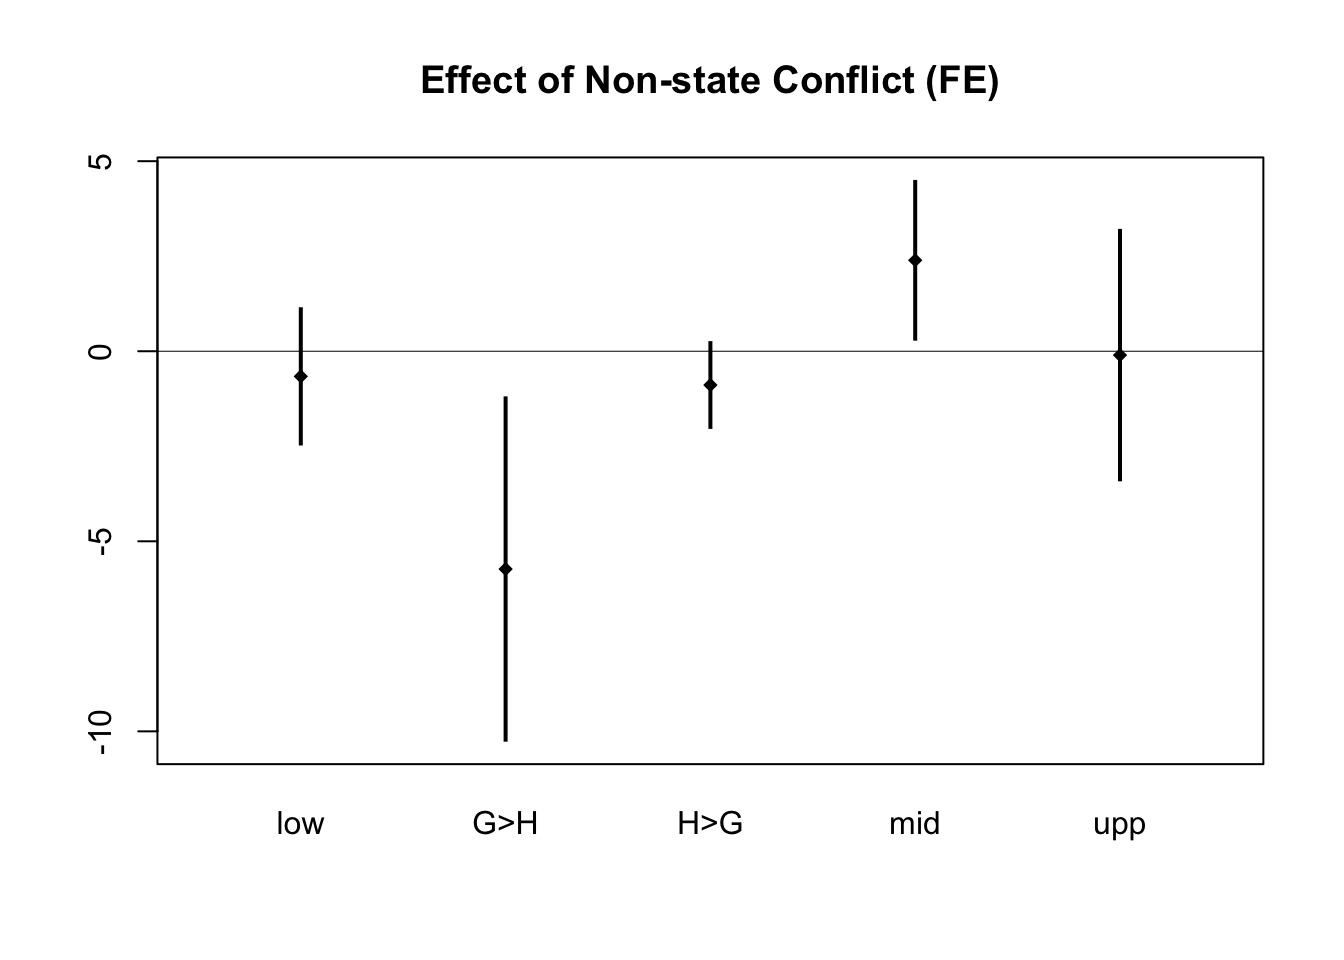
\includegraphics[width=0.45\textwidth]{figures/int_life_exp_nsc_incidence-3.png}
    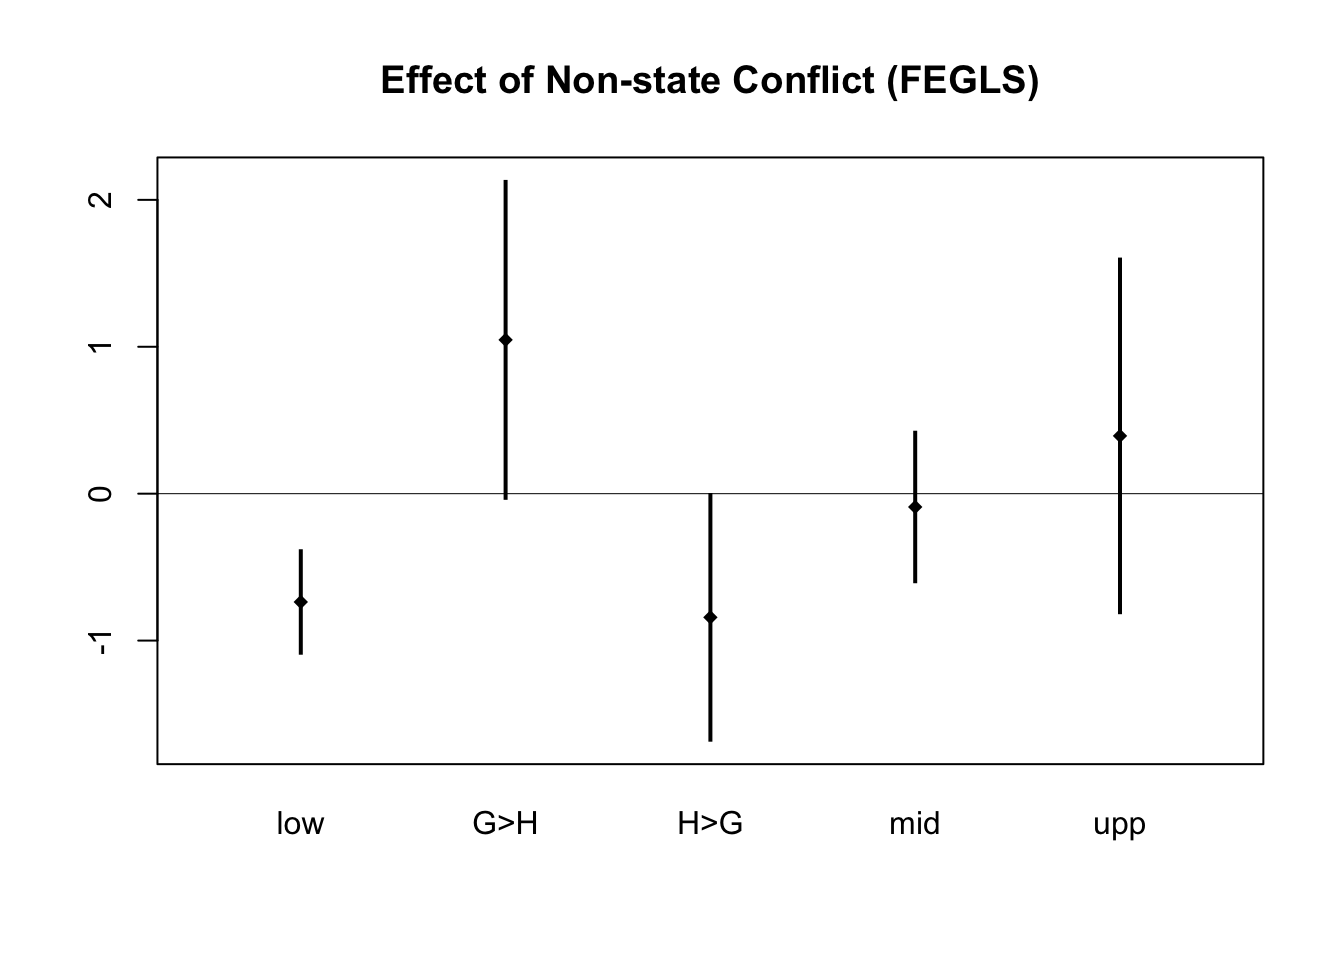
\includegraphics[width=0.45\textwidth]{figures/int_life_exp_nsc_incidence-4.png}
\end{figure}
\begin{figure}[!htb]
    \centering
    \caption{Effect of non-state conflict deaths on life expectancy (with violence controls)}
    \label{int_life_exp_nsc_deaths}
    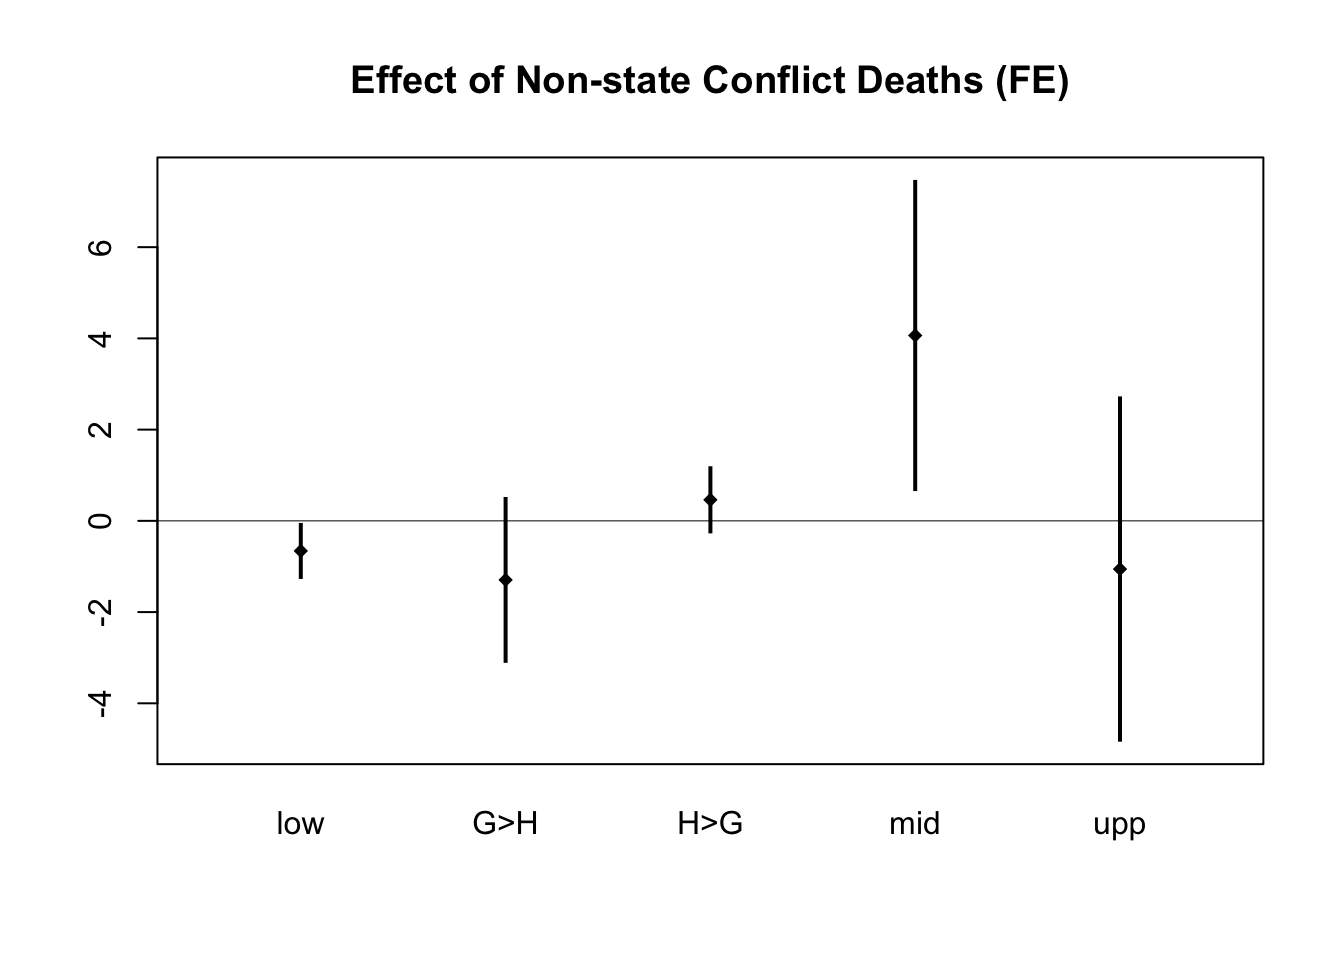
\includegraphics[width=0.67\textwidth]{figures/int_life_exp_nsc_deaths-3.png}
\end{figure}

Both non-state conflict incidence and deaths are associated with a worse IMR in the G>H classification and, in the case of deaths, in the low classification, and with an improved IMR in the mid classification, providing support for vicious and virtuous cycles in some models, as shown in \Cref{int_imr_nsc_incidence} and \Cref{int_imr_nsc_deaths}. The results for the UFMR are similar but weaker (not shown).
The results for some models of DALYs are somewhat supportive of vicious and virtuous cycles involving non-state conflict but these are not robust to the choice of estimator or the inclusion of controls for other types of violence.

\begin{figure}[!htb]
    \centering
    \caption{Effect of non-state conflict on IMR (with violence controls)}
    \label{int_imr_nsc_incidence}
    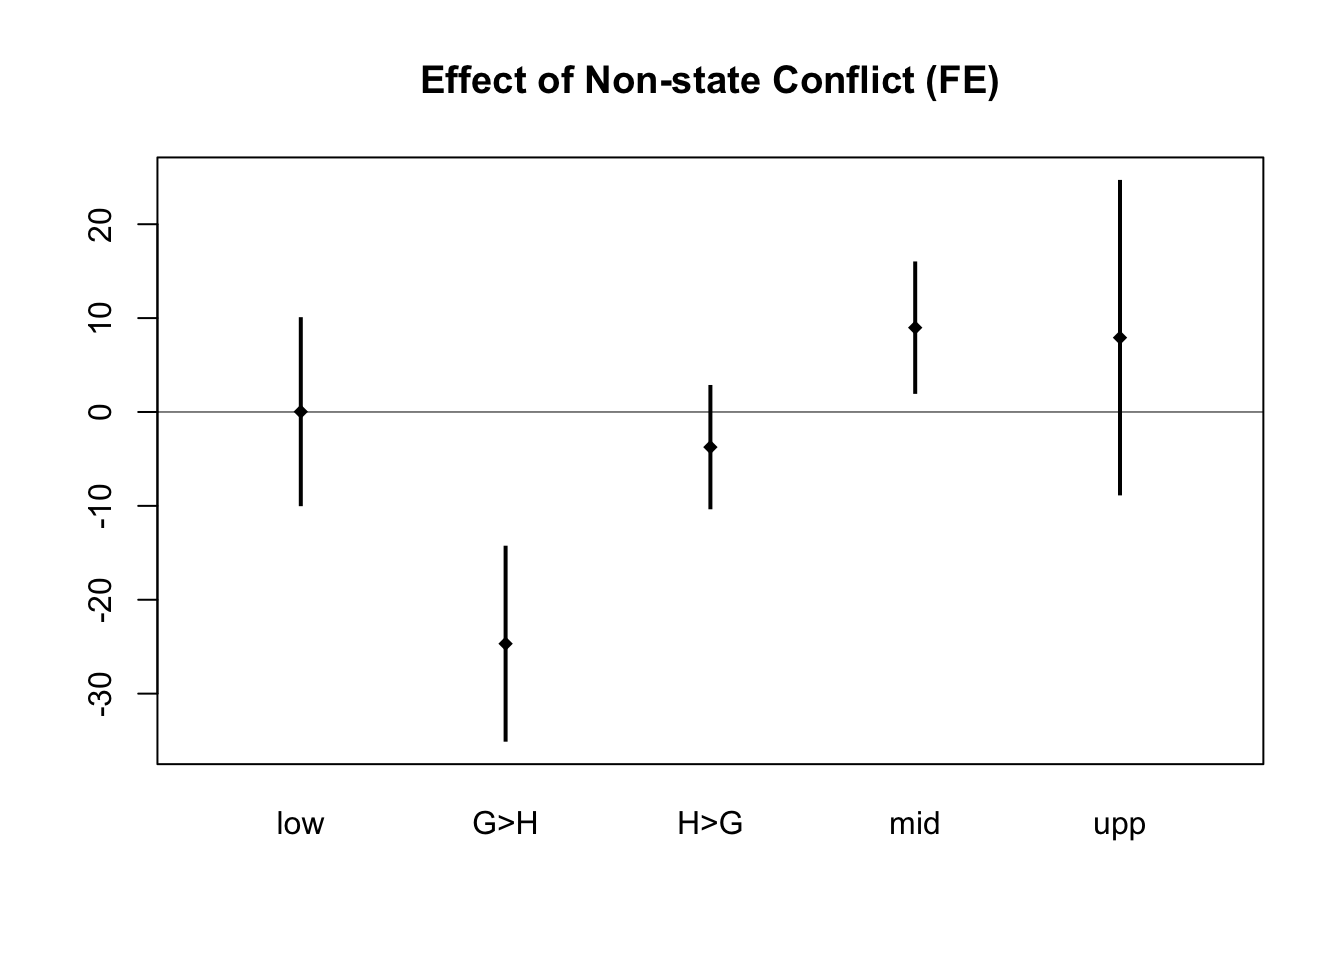
\includegraphics[width=0.67\textwidth]{figures/int_imr_nsc_incidence-3.png}
\end{figure}
\begin{figure}[!htb]
    \centering
    \caption{Effect of non-state conflict deaths on IMR (with violence controls)}
    \label{int_imr_nsc_deaths}
    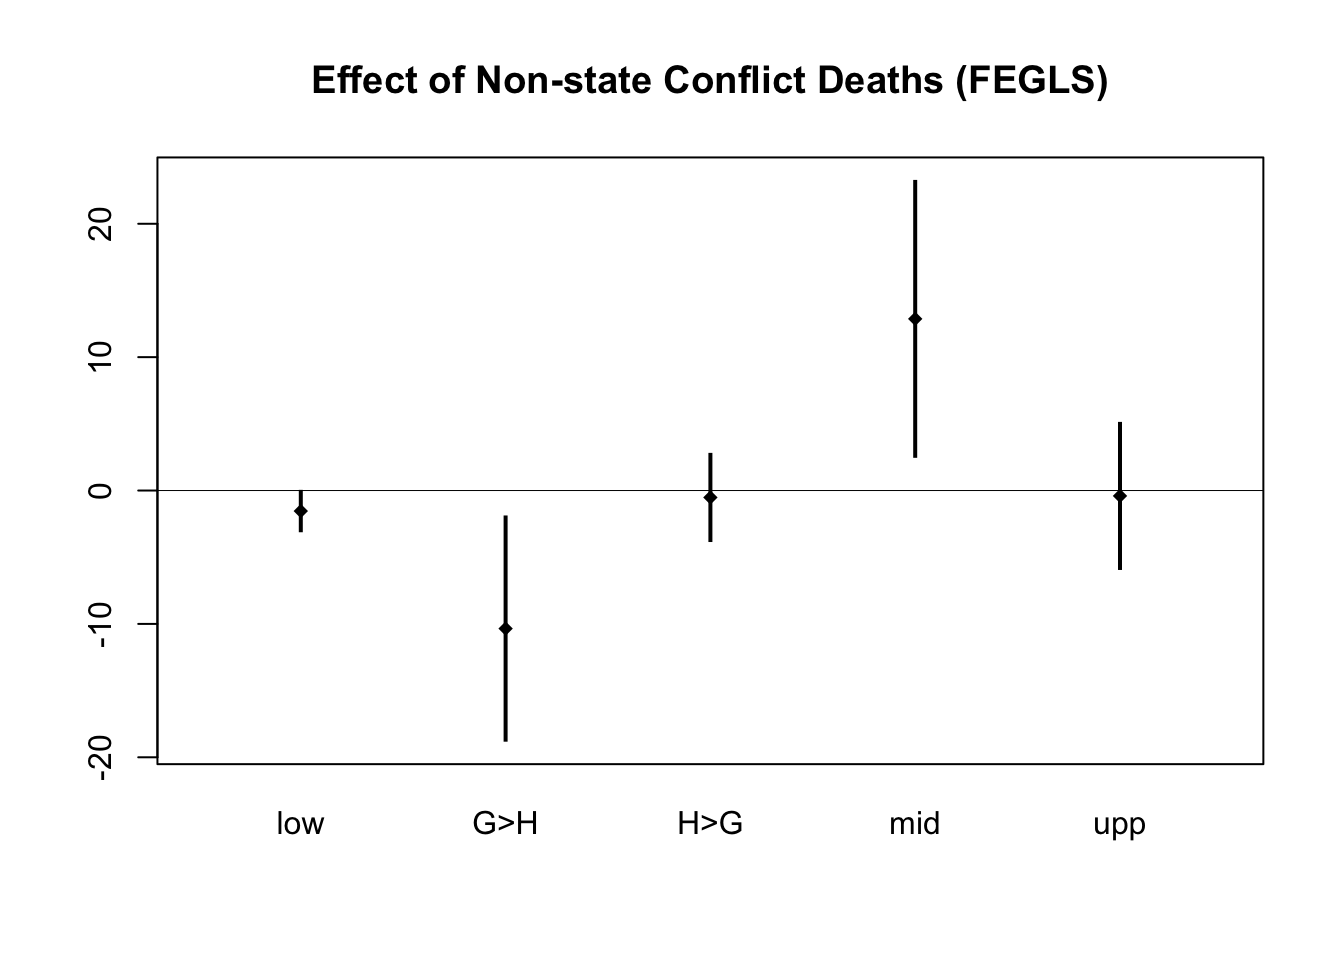
\includegraphics[width=0.67\textwidth]{figures/int_imr_nsc_deaths-4.png}
\end{figure}

With respect to gender outcomes, the models of the MYS ratio often contradict the vicious and virtuous cycles framework, as in some models both non-state conflict incidence and deaths are associated with improvements in lower classifications (not shown).
Non-state conflict deaths are associated with improvements in the AFR in the H>G and upper classifications in \Cref{int_asfr_nsc_deaths}, consistent with virtuous cycles.
Deaths are also associated with with better GIIs, particularly in the low, H>G and upper classifications in \Cref{int_gii_nsc_deaths}, and these effects are difficult to statistically distinguish from each other.
Overall, non-state conflict appears to have less systematic effects on gender and health outcomes than some other types of violence.

\begin{figure}[!htb]
    \centering
    \caption{Effect of non-state conflict deaths on AFR (with violence controls)}
    \label{int_asfr_nsc_deaths}
    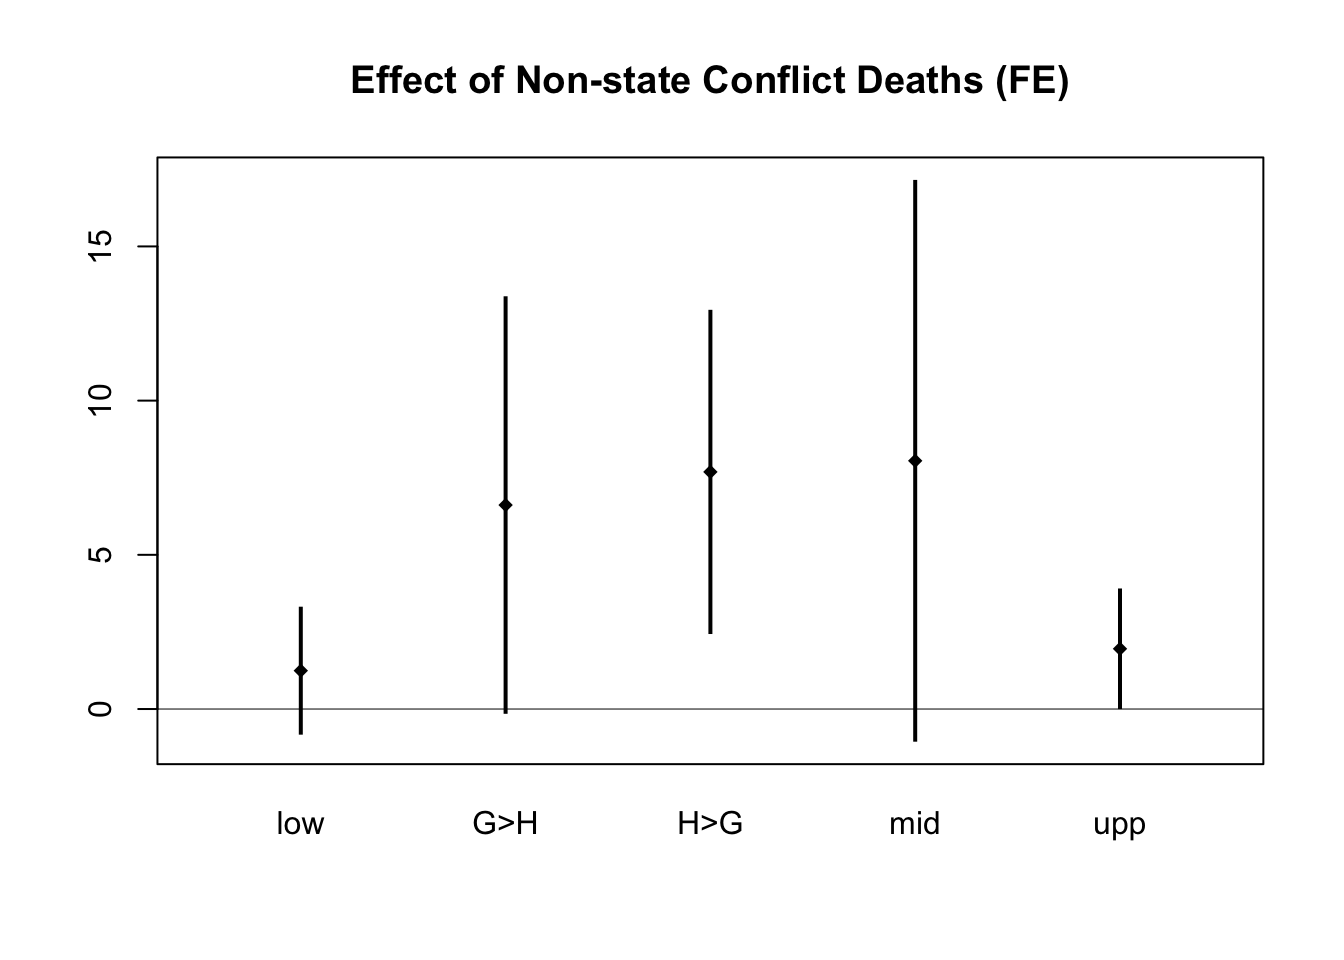
\includegraphics[width=0.67\textwidth]{figures/int_asfr_nsc_deaths-3.png}
\end{figure}

\begin{figure}[!htb]
    \centering
    \caption{Effect of non-state conflict deaths on GII (with violence controls)}
    \label{int_gii_nsc_deaths}
    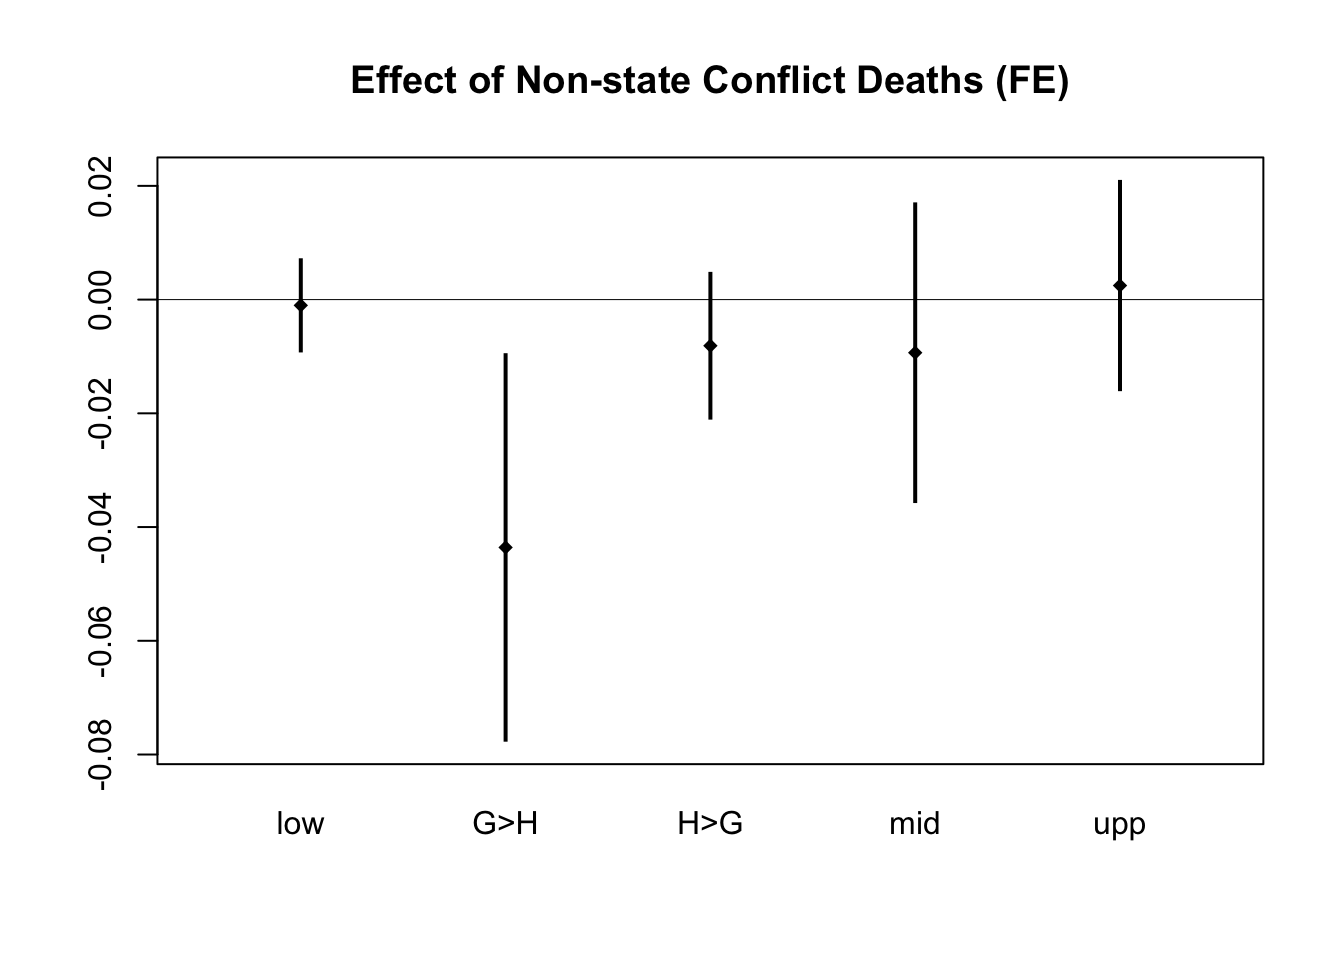
\includegraphics[width=0.67\textwidth]{figures/int_gii_nsc_deaths-3.png}
\end{figure}

\subsubsection{Statistical effects of homicides}

Homicides also represent societal violence but, unlike non-state conflict, not necessarily between organized groups.
The evidence for vicious cycles between health outcomes and homicides is limited.
Unsurprisingly, the models of life expectancy indicate that homicides are associated with declines even in higher classifications (not shown).
In \Cref{int_imr_homicides}, homicides are associated with a worsening IMR in only the G>H classification, and an improvement in the upper classification, depending on the estimator used, and the results are similar and somewhat stronger for the UFMR (not shown).
In some models, homicides are associated with worse DALYs in the low and H>G classifications, consistent with vicious cycles.

\begin{figure}[!htb]
    \centering
    \caption{Effects of homicides on IMR}
    \label{int_imr_homicides}
    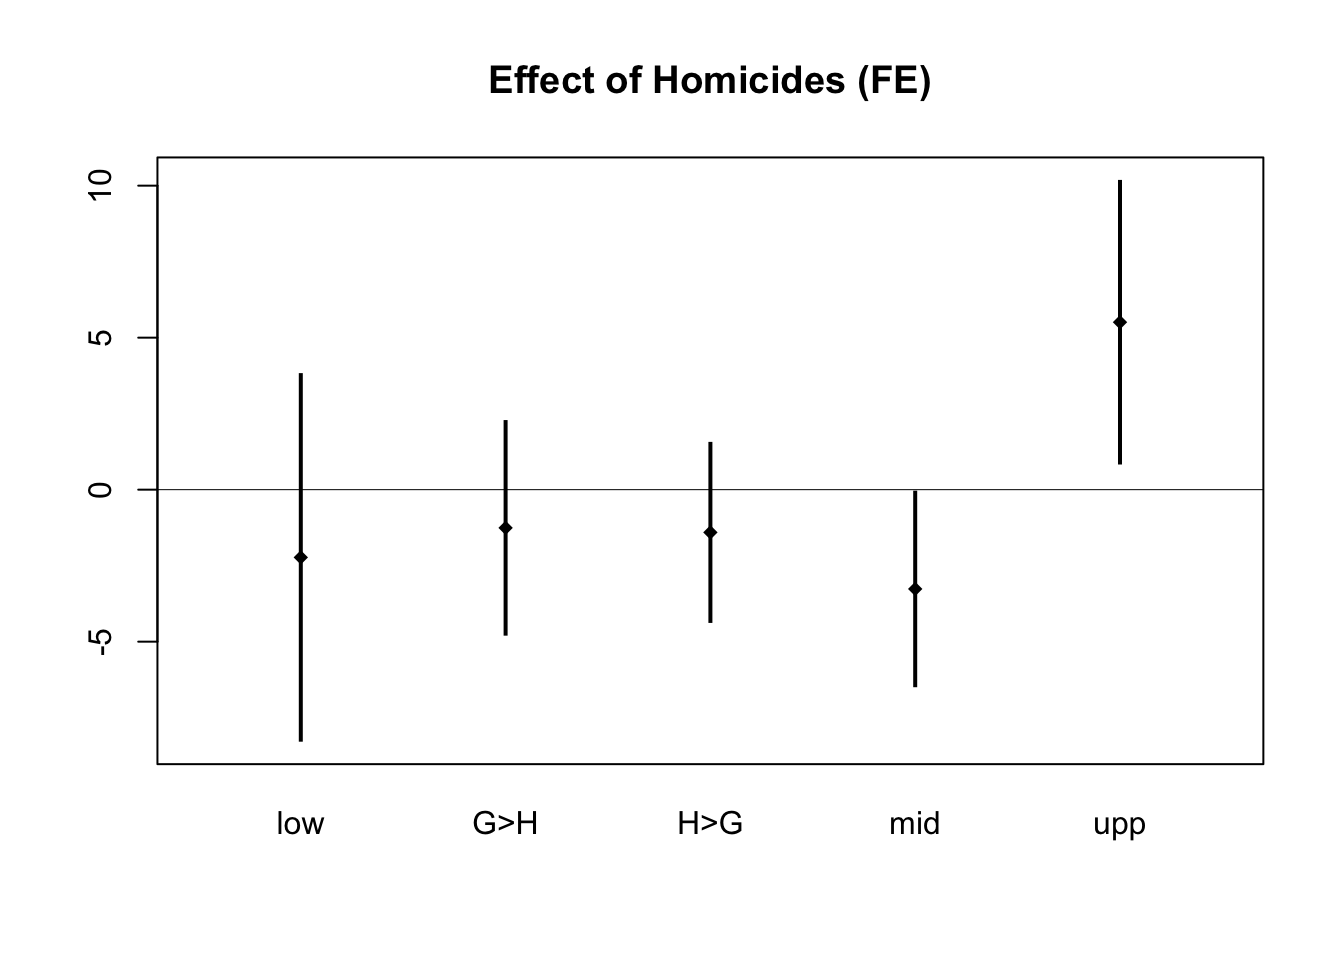
\includegraphics[width=0.45\textwidth]{figures/int_imr_homicides-3.png}
    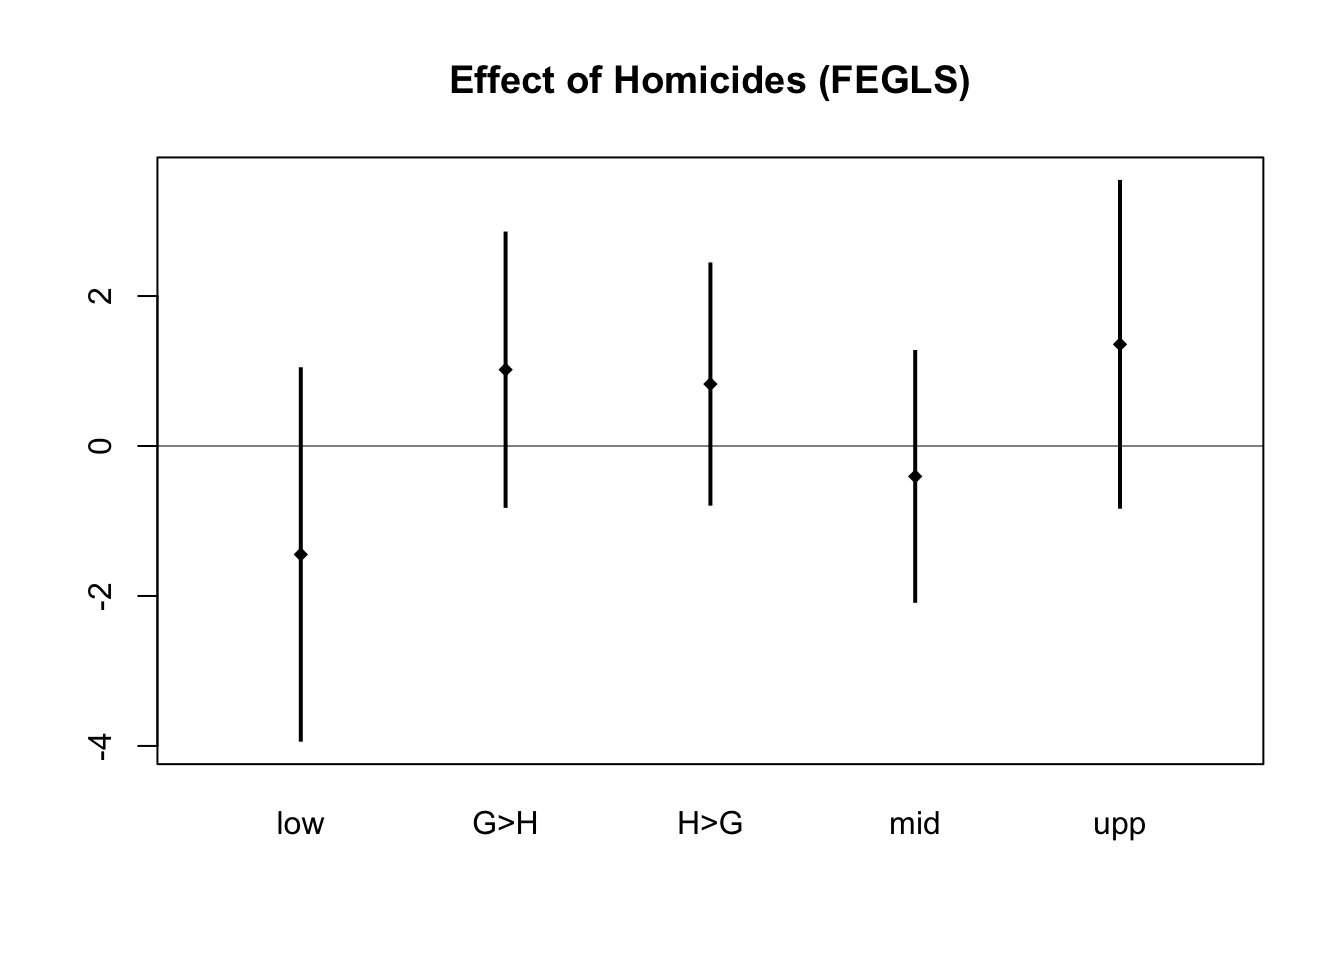
\includegraphics[width=0.45\textwidth]{figures/int_imr_homicides-4.png}
\end{figure}

\begin{figure}[!htb]
    \centering
    \caption{Effects of homicides on DALYs}
    \label{int_daly_homicides}
    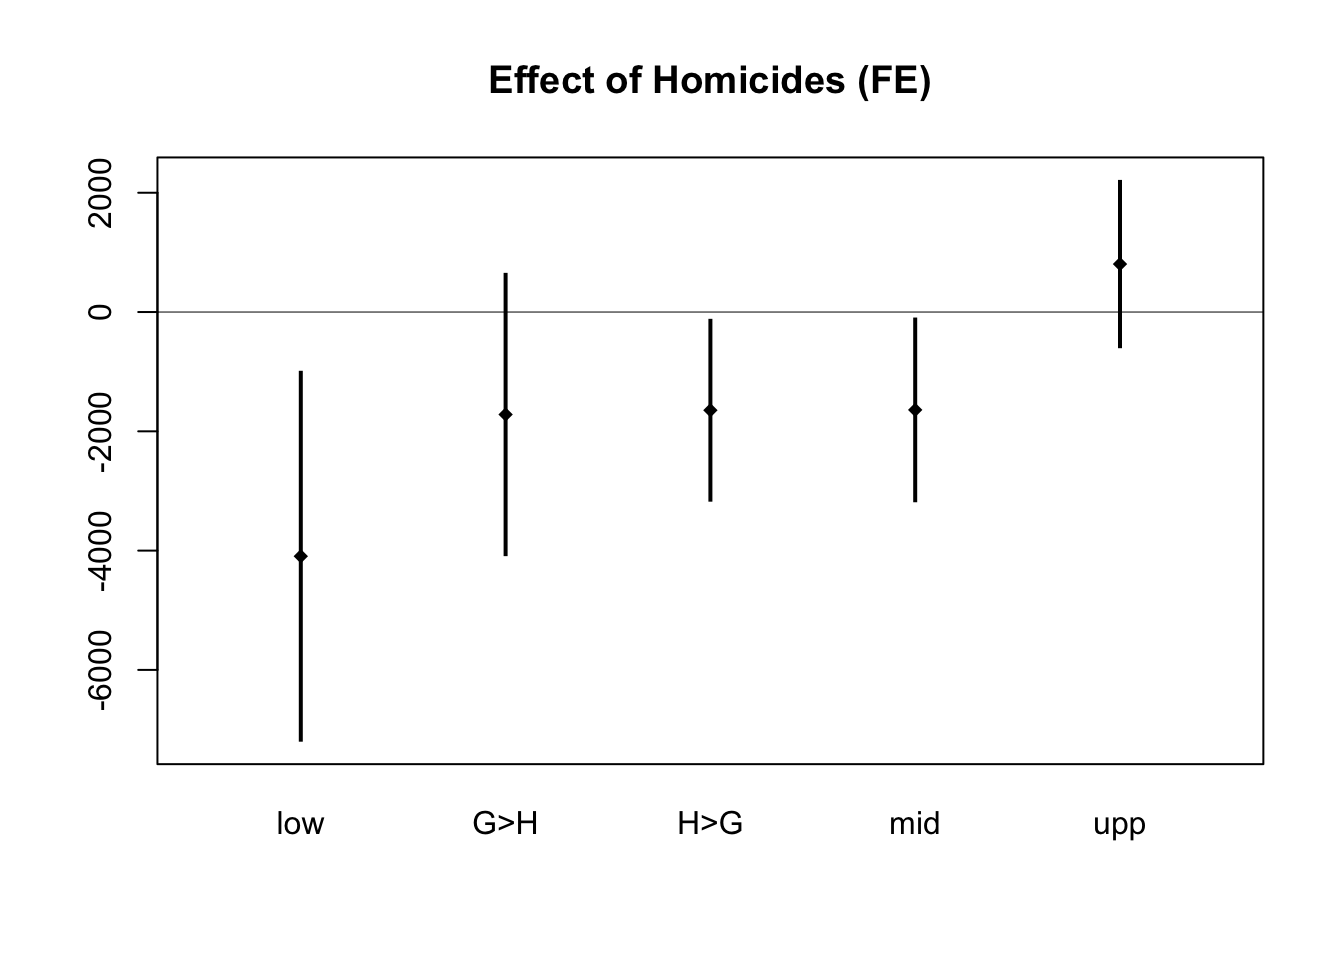
\includegraphics[width=0.45\textwidth]{figures/int_daly_homicides-3.png}
    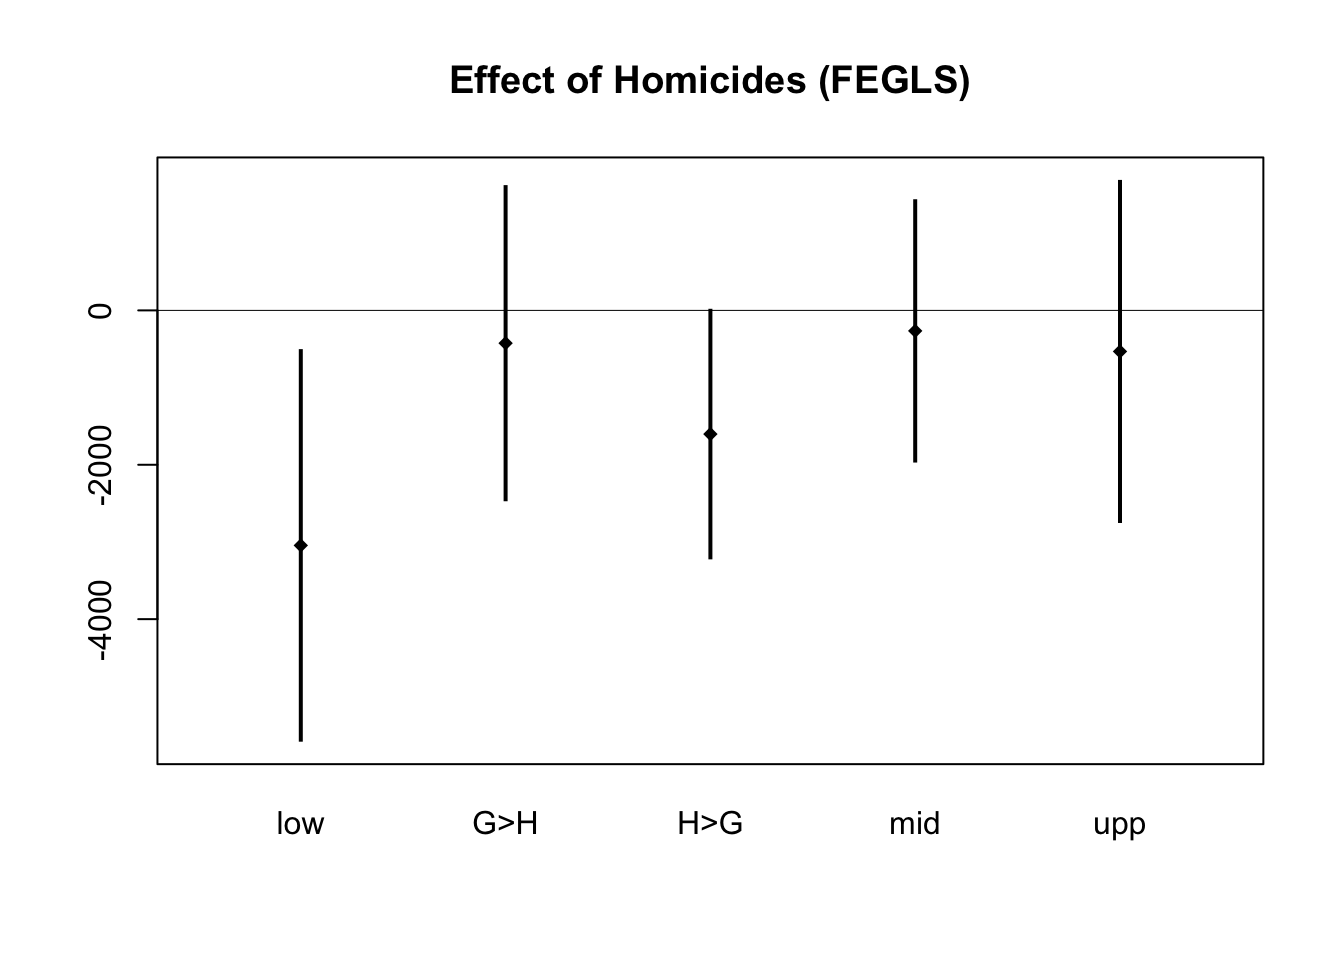
\includegraphics[width=0.45\textwidth]{figures/int_daly_homicides-4.png}
\end{figure}

In models of gender outcomes, the findings are highly variable and not robust to the choice of estimator or the inclusion of controls for other types of violence, often leading to contradictory associations across specifications.
Some models do support vicious and virtuous cycles.
For instance, homicides are associated with a decreased MYS ratios in the FEGLS model, and the interaction effects in \Cref{int_mys_homicides} show worse MYS ratios in the low and mid classifications, compared to an improved ratio in the upper classification, but again these results are not robust to accounting for other types of violence.
However, interesting evidence is provided by the FEGLS estimator in \Cref{int_gii_homicides}, where homicides are associated with a worse GII in the G>H classification, and a better GII in the H>G classification.

\begin{figure}[!htb]
    \centering
    \caption{Effects of homicides on MYS ratio}
    \label{int_mys_homicides}
    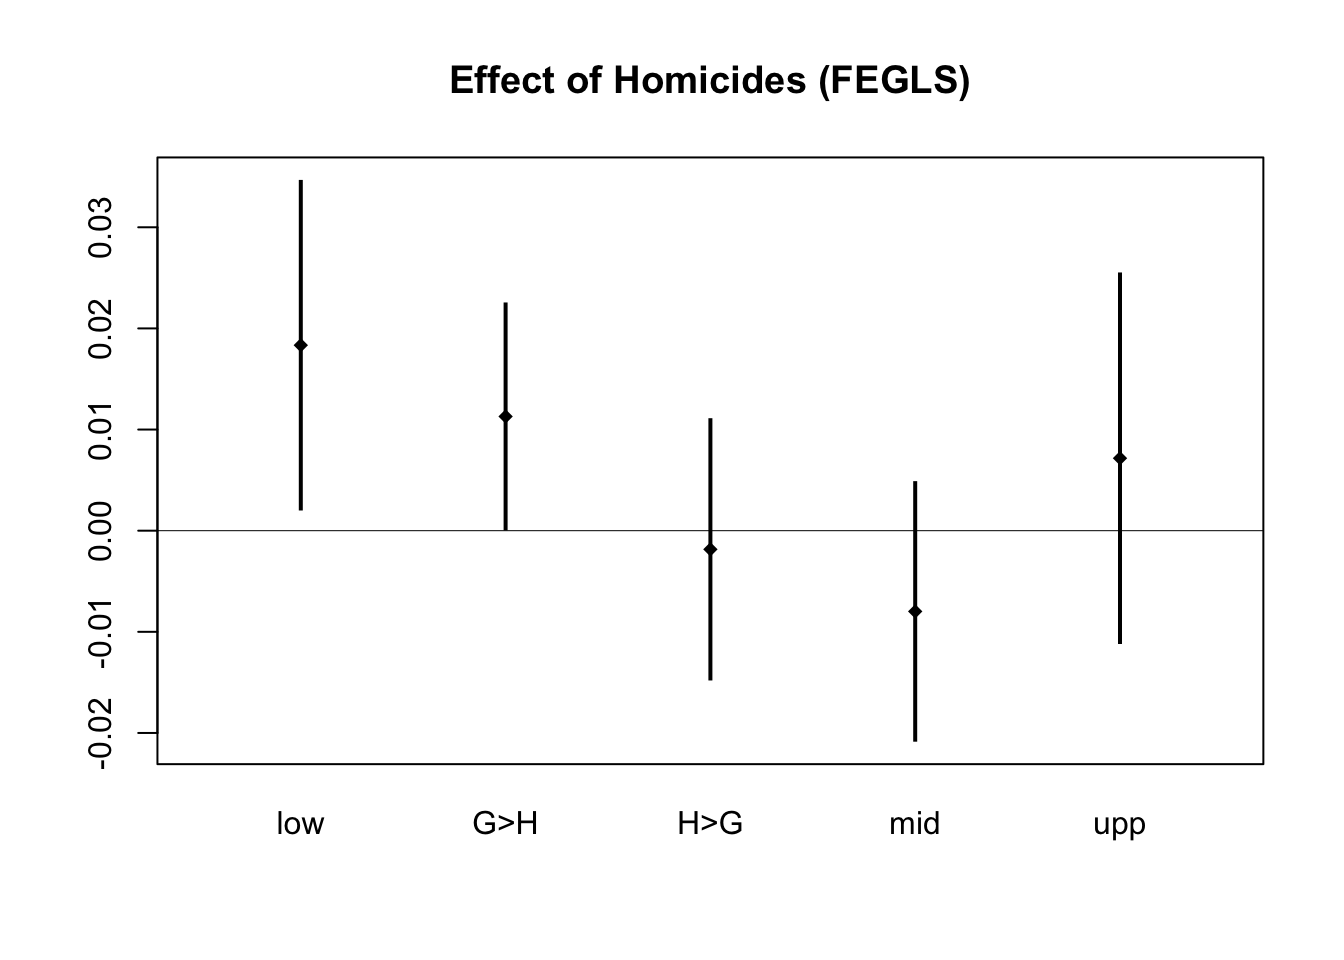
\includegraphics[width=0.67\textwidth]{figures/int_mys_homicides-2.png}
\end{figure}
\begin{figure}[!htb]
    \centering
    \caption{Effects of homicides on GII}
    \label{int_gii_homicides}
    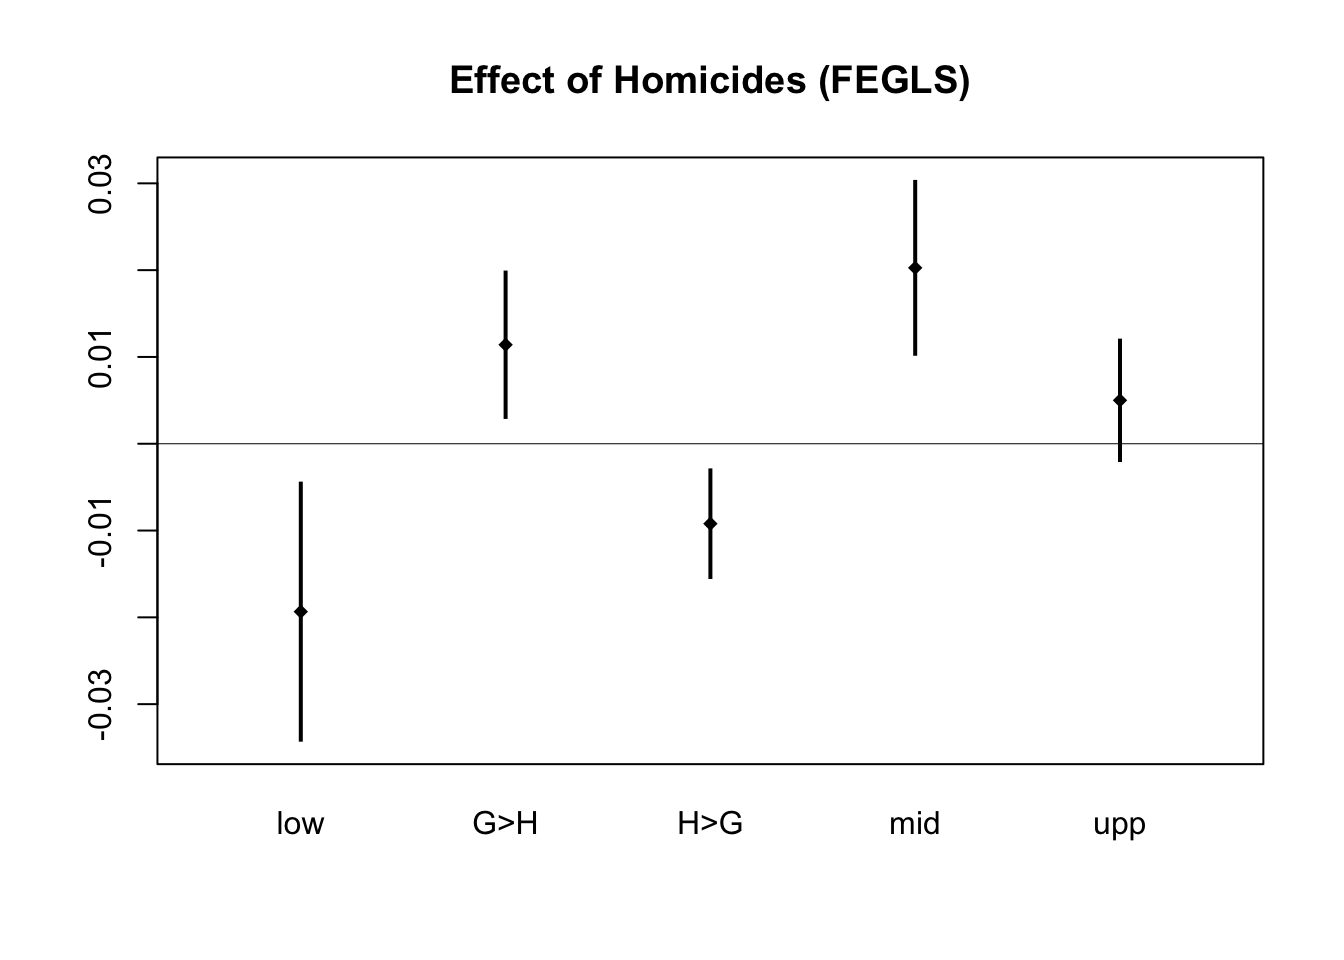
\includegraphics[width=0.67\textwidth]{figures/int_gii_homicides-4.png}
\end{figure}

\clearpage
\begin{sidewaystable}[!htbp]
\small
\centering
\caption{Summary of findings on health and gender outcomes: societal violence interactions}
\label{table_hg_societal}
\begin{tabular}{lccccccccccc}
\toprule
                                       & Life                  & IMR         & UFMR        & DALYs     & MYS                     & AFR       & Labor part. & GII \\
                                       & Expectancy            &             &             &           & ratio                   &           & ratio       & \\
\midrule
non-state conflict incidence           & $-$ \ddag             &             &             &           & $+$ \ddag               &           &             & \\
--- low classification interaction     & $-$ \ddag             &             &             &           & $+$ \ddag               &           &             & \\
--- G$>$H classification interaction   & $-$ \dag              & $-$ \dag    & $-$ \dag    & $-$ \dag  &                         &           &             & \\
--- H$>$G classification interaction   &                       & $+$ \dag    & $-$ \dag\ * &           & $+$ \ddag               &           &             & \\
--- mid classification interaction     & $+$ \dag              & $+$ *       &             &           & $+$ \ddag               &           &             & \\
--- upp classification interaction     & $-$ \ddag             &             &             &           &                         &           &             & \\
\midrule
non-state conflict deaths              & $-$ \ddag             & $-$ \ddag   &             & $-$ \ddag & $+$ \ddag               & $+$ \dag  &             & $-$ \\
--- low classification interaction     & $-$ \dag\ / *         & $-$ \ddag   &             & $-$ \ddag & $+$ \ddag               &           & $+$ \dag    & $-$ \dag \\
--- G$>$H classification interaction   & $-$ \dag              & $-$         & $-$ *       &           & $-$ \dag                &           & $+$ \dag    & \\
--- H$>$G classification interaction   & $+$ \ddag\ *          & $-$ \dag\ * & $-$ \dag\ * &           & $+$ \ddag               & $+$ \dag  &             & $-$ \dag \\
--- mid classification interaction     & $+$ \dag\ / $-$ \ddag & $+$         & $+$         &           & $-$ \ddag               &           &             & \\
--- upp classification interaction     & $-$ \ddag\ *          & $+$ \dag    & $+$ \dag    & $+$ \dag  &                         & $+$ \dag  &             & $+$ \dag\ * \\
% \midrule
% non-state conflict civilian deaths \\
% --- low classification interaction   & $+$ \ddag             &             &             & $-$ \ddag & $+$                     &           & $+$ \dag    & \\
% --- G$>$H classification interaction & $+$ \dag\ / *         &             &             & $-$ \ddag &                         &           &             & $+$ \ddag \\
% --- H$>$G classification interaction &                       & $-$ \dag\ * & $-$ \dag\ * & $-$ \ddag & $+$ \ddag               & $+$ \dag  & $-$         & \\
% --- mid classification interaction   & $+$ \dag\ / $-$ \ddag & $+$         & $+$         & $+$       & $-$ \ddag               & $+$ \dag  &             & \\
% --- upp classification interaction   & $+$                   & $+$ \dag    & $+$ \dag    & $+$ \dag  & $+$                     & $+$ \dag  & $+$ \dag    & \\
\midrule
homicides                              &                       &             &             &           & $-$ \ddag               &           &             & \\
--- low classification interaction     &                       &             &             & $-$ \ddag & $-$ \ddag\ *            &           &             & $-$ \ddag \\
--- G$>$H classification interaction   & $-$ \ddag             & $-$ \ddag   & $-$ \ddag   &           &                         & $+$       &             & $+$ \ddag \\
--- H$>$G classification interaction   & $-$                   &             & $-$ \dag    & $-$       &                         &           &             & $-$ \ddag \\
--- mid classification interaction     &                       &             &             &           & $+$ \ddag\ * / $-$ \dag & $-$ \ddag &             & $+$ \ddag \\
--- upp classification interaction     & $-$ / $+$ \ddag\ *    & $+$ \dag    & $+$ \dag    &           & $+$ \ddag\ *            &           &             & \\
\bottomrule
\end{tabular}
\caption*{\footnotesize Legend:
$+$, $-$ statistically significant effects;
\dag\ FE model only;
\ddag\ FEGLS model only;
* model does not include controls for other types of violence.}
\end{sidewaystable}

\clearpage

\subsection{Analyses of violence outcomes}
\label{results_violence}

This section summarizes the findings of the models of violence outcomes. These are structured analogously to the models of health and gender outcomes. They examine the statistical effects of individual gender and health variables, of the classifications, and of their interactions with the lagged violence variables. As discussed in \Cref{classifications}, the former set of models test the effects of gender and health outcomes on violence, while the interactions test the effects of past violence in particular health and gender contexts on current violence, providing evidence on three-way relationships.
\Cref{table_panel_violence} provides a summary of the findings, and the main findings are discussed below.

\begin{sidewaystable}[htbp]
\footnotesize
\centering
\caption{Summary of findings on violence outcomes}
\label{table_panel_violence}
\begin{tabular}{lccccccccccc}
\toprule
                            & Internal      & Internal  & Conflict    & OSV       & OSV       & State      & Extra-            & NSC       & NSC       & NSC         & Homicides \\
                            & conflict      & conflict  & civilian    & incidence & deaths    & repression & judicial          & incidence & Deaths    & Civilian    & \\
                            & incidence     & deaths    & deaths      &           &           & (LPI)      & killings          &           &           & Deaths      & \\
\midrule
Life expectancy             & $-$ \ddag     &           & $+$ \ddag   & $-$       & $+$ \ddag & $-$ \ddag  & $-$ \ddag         &           &           &             & \\
Infant mortality rate       & $-$           &           & $-$ \ddag   & $-$       &           & $-$        & $-$ \ddag         &           &           &             & \\
MYS ratio                   & $-$           &           & $-$ \ddag   & $-$ \ddag &           & $-$        & $-$               &           &           &             & \\
Adolescent fertility rate   & $-$ \ddag     &           & $-$ \ddag   &           &           & $-$        &                   & $-$ \dag  &           &             & \\
\midrule
low classification          & reference     & reference & reference   & reference & reference & reference  & reference         & reference & reference & reference   & reference \\
G$>$H classification        & $-$ \ddag     &           &             &           &           &            & $+$ \ddag         &           &           &             & \\
H$>$G classification        & $-$           &           &             &           &           &            & $+$ \ddag         & $+$ \dag  &           &             & $-$ \ddag \\
mid classification          & $-$ \ddag     &           &             &           &           &            & $+$ \ddag         &           &           &             & \\
upp classification          & $-$           &           &             &           &           &            & $+$ \ddag         &           &           &             & $-$ \ddag \\
\midrule
interactions with lagged DV \\
--- low classification      & $+$ *         &           &             & $+$ \dag  & $-$ \ddag &            & $+$ \ddag (most)  & $-$ \ddag & $+$       & $-$ \ddag   & $+$ \ddag\ or * \\
--- G$>$H classification    & $+$ * (most)  &           &             &           &           & $+$ \ddag  & $+$ \ddag         & $-$       &           & $-$ \ddag * & $+$ \\
--- H$>$G classification    & $+$ *         &           & $+$ \dag    & $+$ \dag  &           &            & $+$ \ddag (least) &           & $-$ \ddag &             & $+$ \dag\ or * \\
--- mid classification      & $+$ * (least) &           &             & $+$       &           & $+$ \ddag  & $+$ \ddag         & $+$ \dag  & $+$       & $+$ \dag    & $+$ (most) \\
--- upp classification      & $+$ * (most)  & $-$ \ddag & $+$ \ddag * & $-$       &           & $+$ \ddag  & $+$ \ddag         &           &           & $+$ \dag    & $-$ \ddag * / $+$ \dag \\
\bottomrule
\end{tabular}
\caption*{\footnotesize Legend:
$+$, $-$ statistically significant effects;
\dag\ FE model only;
\ddag\ FEGLS model only;
* model does not include controls for other types of violence.}
\end{sidewaystable}


\subsubsection{Internal Conflict}

The models of internal conflict measures provide some evidence for the proposed framework.
Improvements in all four of the main health and gender variables are associated with decreased internal conflict incidence, and all but life expectancy are also associated with decreased internal conflict civilians deaths.
Unexpectedly, on average, an increase in life expectancy is followed by increased civilian deaths.
When the classification indicators are included (with the low classification as the reference category), all other classifications are associated with decreased internal conflict incidence, but the classifications have no significant statistical effects on conflict deaths.
With the one exception, these results are broadly consistent with the framework, but as discussed in \Cref{classifications}, these tests do not allow distinguishing vicious and virtuous cycles from each other or assessing feedback loops involving violence.

\begin{figure}[!htb]
    \centering
    \caption{Effects of past internal conflict deaths on current deaths (with violence controls)}
    \label{int_conflict_deaths}
    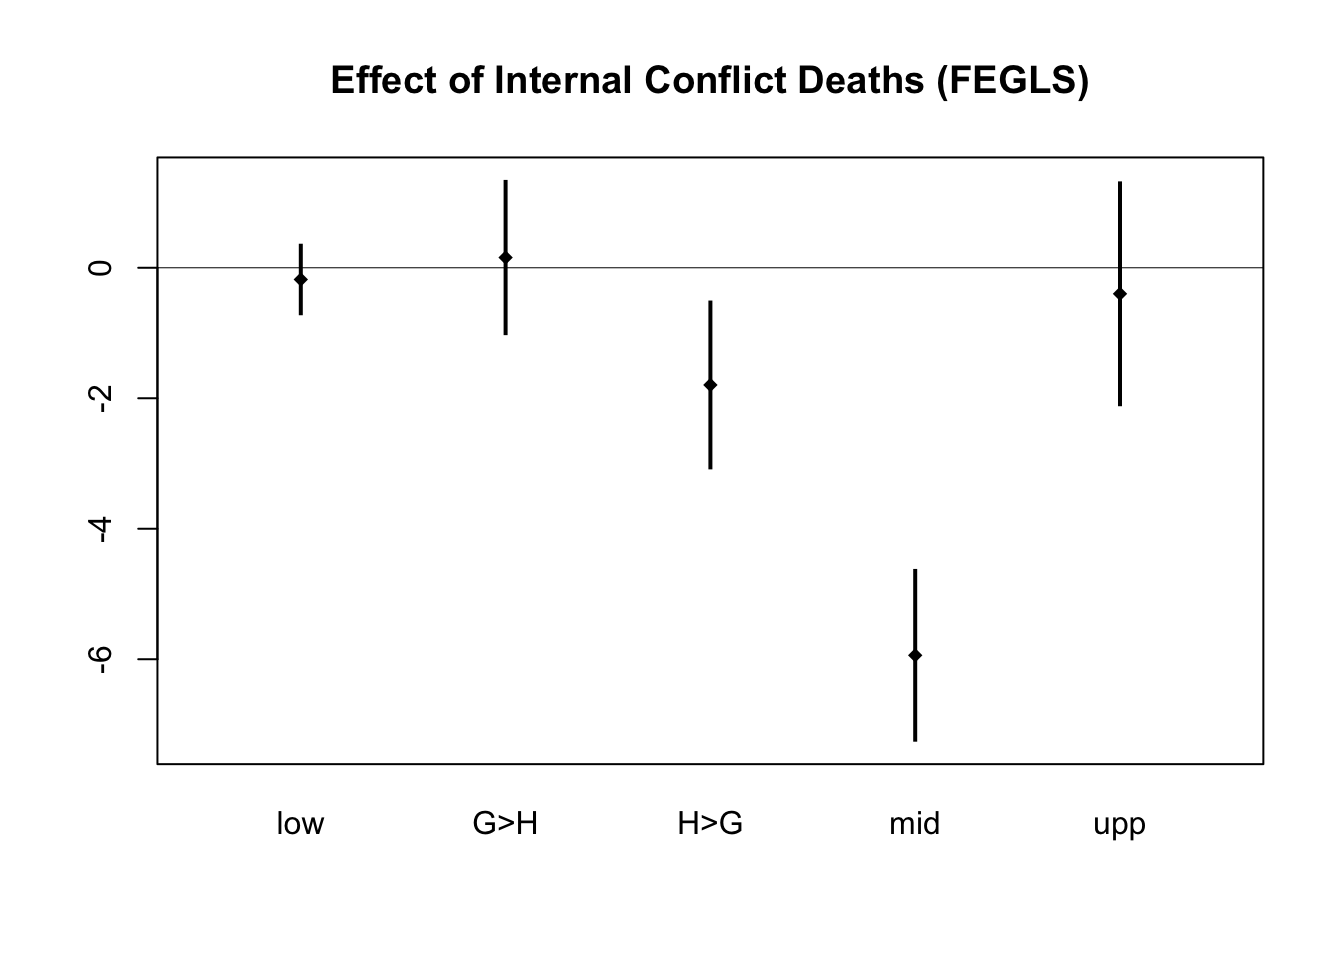
\includegraphics[width=0.67\textwidth]{figures/int_conflict_deaths-4.png}
\end{figure}

The models employing the interactions of the classifications with past conflict provide only limited evidence of such three-way vicious and virtuous cycles, as they either do not show clear differences between the classification groups or show associations that actually contradict virtuous cycles, with one clear exception shown in \Cref{int_conflict_deaths}: past conflict deaths are associated with decreased conflict deaths in the next period in only the upper classification, suggesting that very high health and gender performance may have a dampening effect on conflict deaths, and this effect is clearly statistically distinguishable from all the other classifications.
The models of civilian conflict deaths reveal some associations that contradict virtuous cycles, but these results are not robust to the FEGLS estimator or controlling for other types of violence.

\subsubsection{State repression}

Several different measures are used to examine repressive state violence, with mixed results. There is some support for vicious and virtuous cycles in the models of one-sided violence incidence.
The individual health variables and MYS ratio are associated with decreased incidence, but analogous to the internal conflict results, life expectancy is surprisingly associated with increased one-sided violence deaths.
The classifications on their own do not have clear statistical effects, but their interactions with the lagged dependent variable strongly supports vicious and virtuous cycles in the FE models in \Cref{int_osv_class_controls}: past OSV in the low, H>G and mid classifications is associated with increased incidence in the next period, but decreased OSV in the upper classification.
However, in the FEGLS model, only the interactions with the highest classifications are still statistically significant.
Moreover, in the model of OSV deaths, the interaction with the low classification contradicts expectation, as it is associated with a decrease in subsequent deaths.

\begin{figure}[!htb]
    \centering
    \caption{Effects of past OSV on current incidence (with violence controls)}
    \label{int_osv_class_controls}
    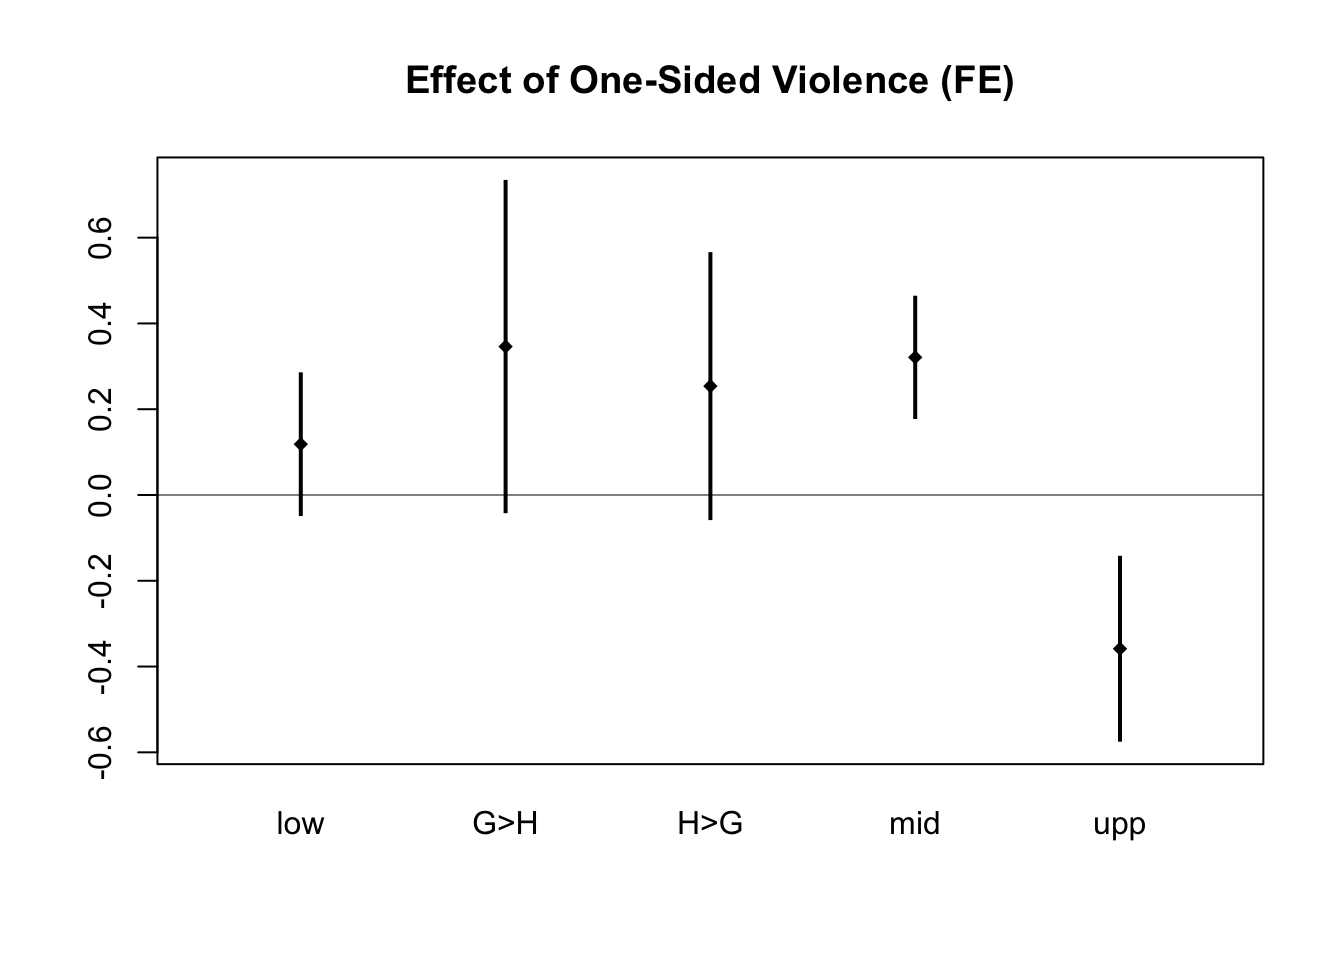
\includegraphics[width=0.45\textwidth]{figures/int_osv-3.png}
    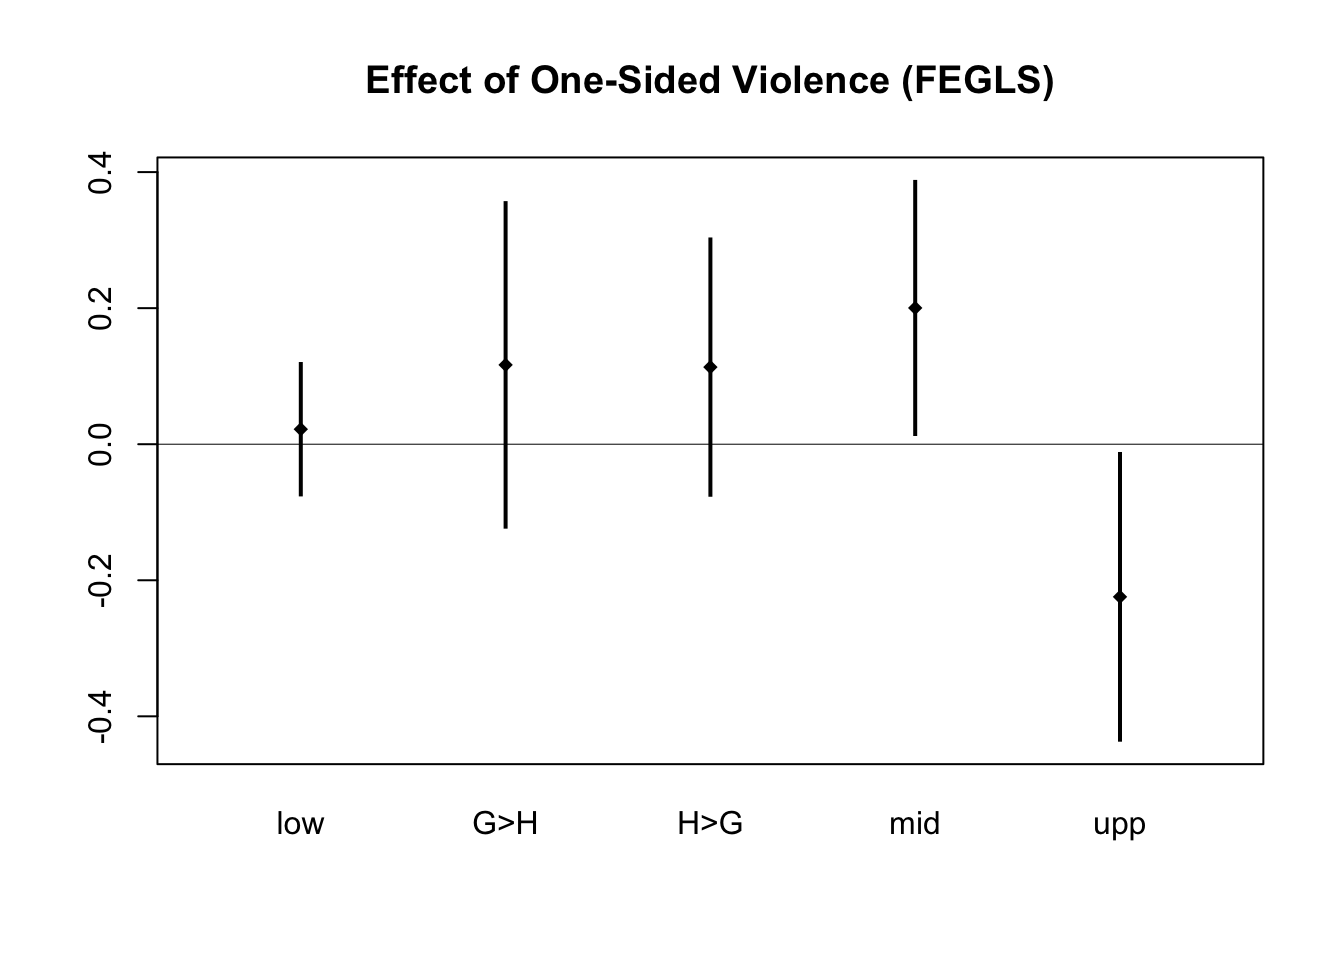
\includegraphics[width=0.45\textwidth]{figures/int_osv-4.png}
\end{figure}

\begin{figure}[htb]
    \centering
    \caption{Effects of past physical integrity violations on current violations (with violence controls)}
    \label{int_lpi_class_controls}
    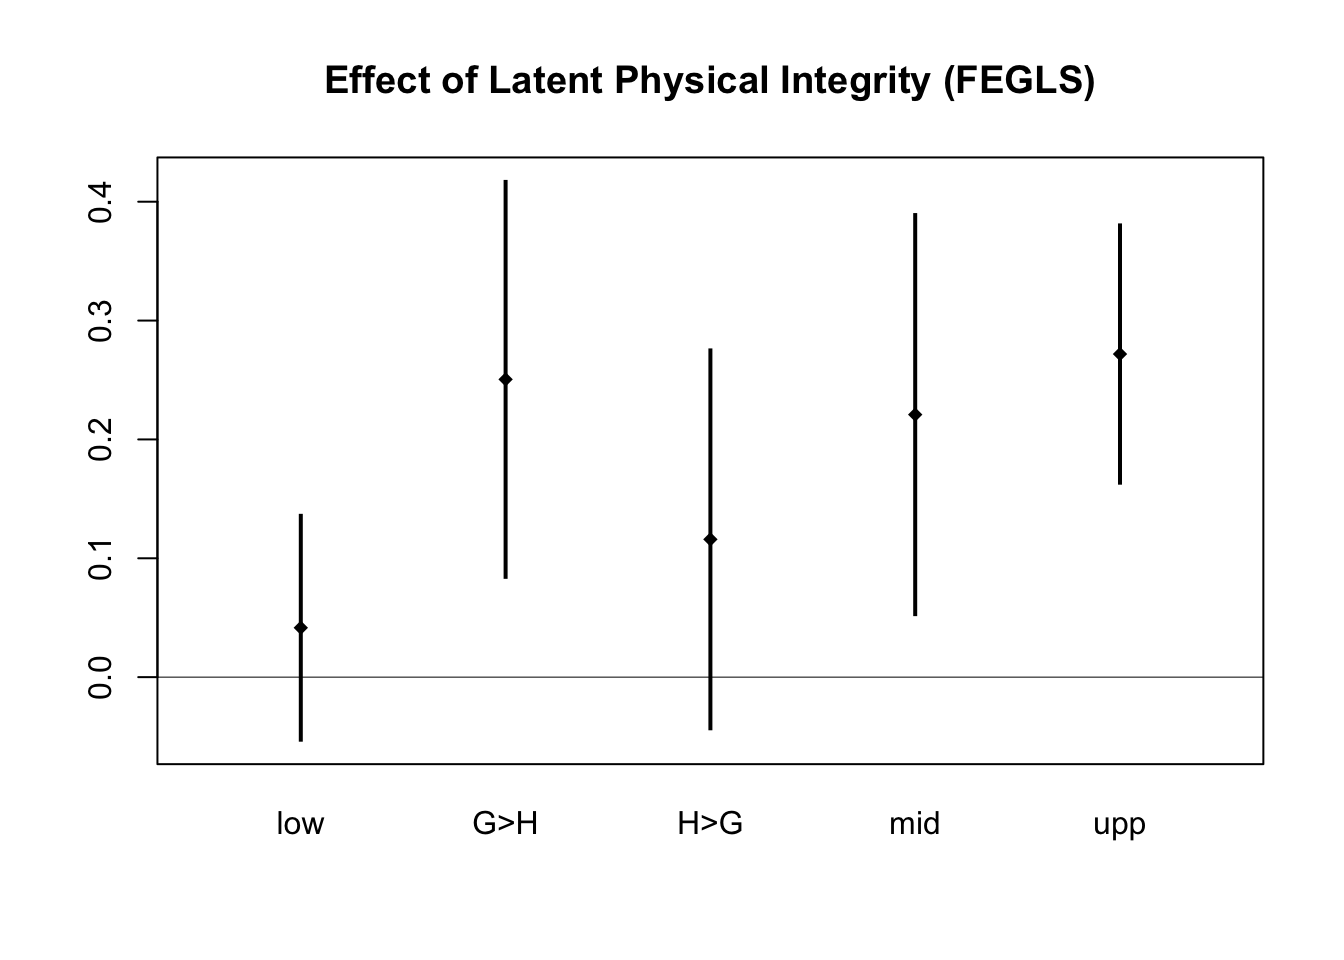
\includegraphics[width=0.67\textwidth]{figures/int_lpi-4.png}
\end{figure}

The results for other measures of violent repression are also mixed.
The individual health variables and the MYS ratio are associated with improvements in latent physical integrity (LPI) and the V-Dem measure of extra-judicial killings, and the AFR also has this association with the LPI. These results are again consistent with vicious and virtuous cycles.
The results for the classification indicators on their own show no clear differences in the LPI models, and their interactions in the FEGLS models contradict expectations, as shown in \Cref{int_lpi_class_controls}, where the low classification is not associated with increased violence, but the mid and upper classifications are.
In the FEGLS models of extra-judicial killings the classifications also have statistically significant effects opposite to what we would expect, but their interactions with the lagged dependent variable in \Cref{int_killings_class} are supportive of vicious and virtuous cycles: while past extra-judicial killings are associated with more current killings across all classifications, the increase is greatest in the low classification, which is statistically distinguishable from those of the H>G, mid, and upper classifications.

\begin{figure}[!htb]
    \centering
    \caption{Effects of past extra-judicial killings on current killings (with violence controls)}
    \label{int_killings_class}
    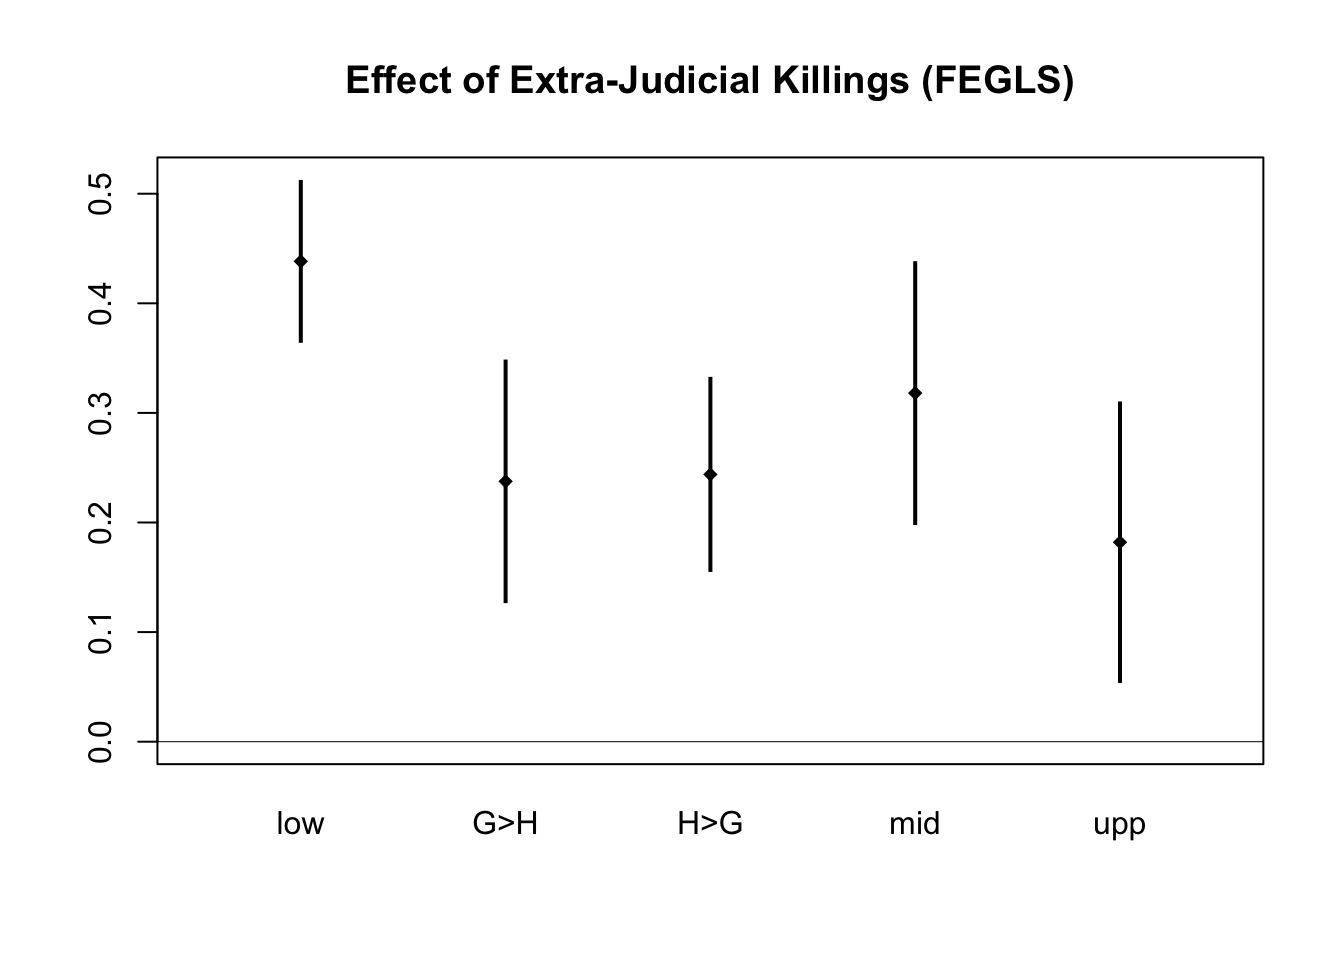
\includegraphics[width=0.67\textwidth]{figures/int_killings-4.png}
\end{figure}

\subsubsection{Non-state conflict}

In the models of non-state conflict incidence and deaths, only improvements in the AFR are associated with decreased incidence in the FE model. Neither the other individual health and gender variables nor the classifications have statistically distinguishable effects. The models with interactions of non-state conflict incidence or civilian deaths with the classifications contradict vicious cycles because in the low and G>H classifications there are statistically significant associations with less violence in several models.
The interactions with total non-state conflict deaths provide a partial exception in \Cref{int_deaths_nsc}: past deaths are associated with increased deaths in the next period in the low and mid classifications, but decreased deaths in the H>G classifications, which may reflect a virtuous cycle in the latter.
Otherwise, the models of non-state conflict and deaths provide limited evidence for the proposed framework.

\begin{figure}[!htb]
    \centering
    \caption{Effects of past non-state conflict deaths on current deaths}
    \label{int_deaths_nsc}
    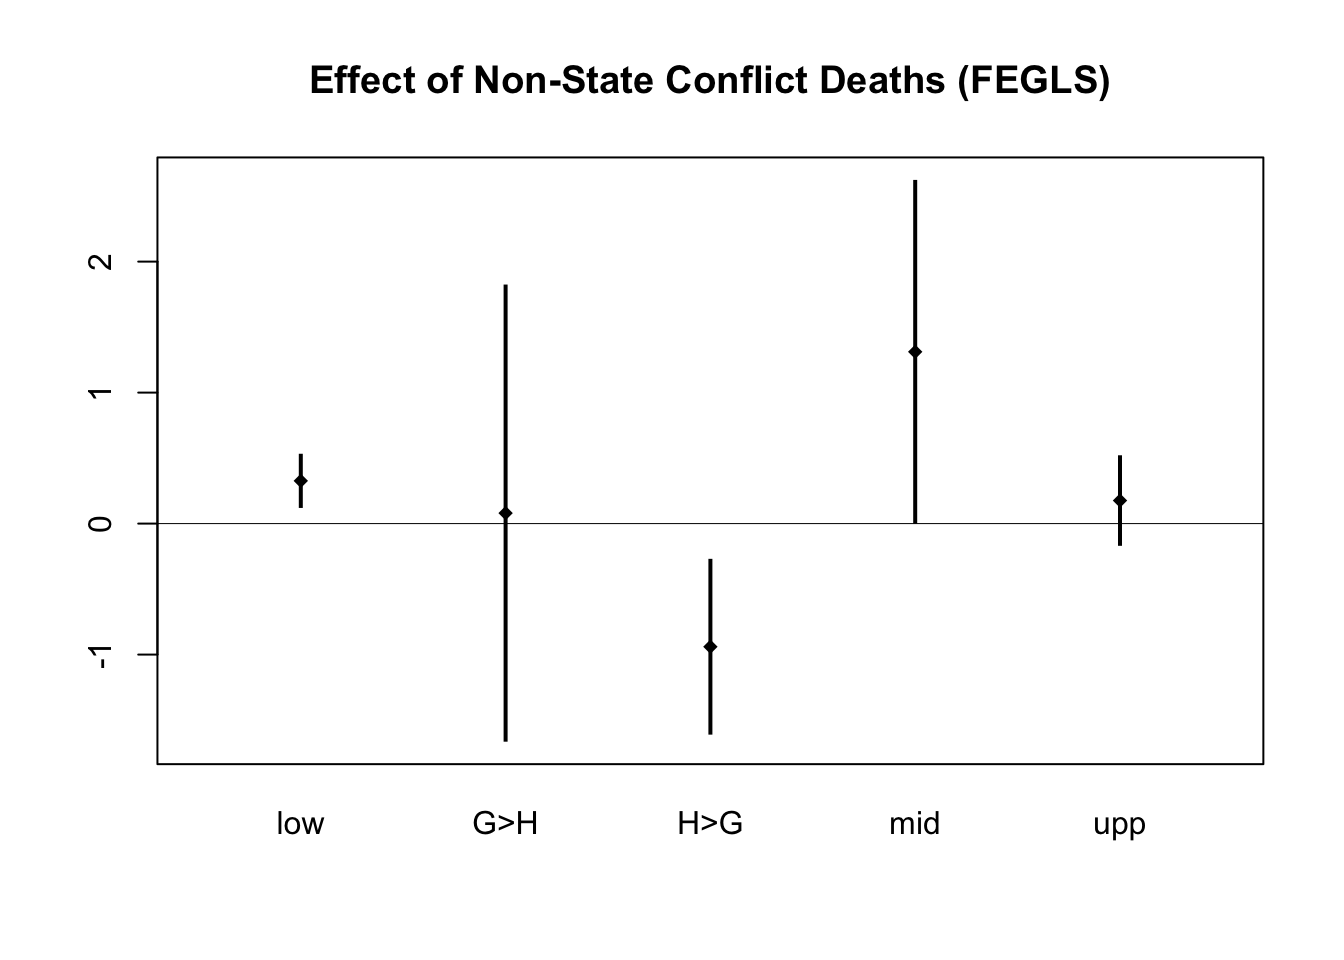
\includegraphics[width=0.67\textwidth]{figures/int_nsc_deaths-4.png}
\end{figure}

\subsubsection{Homicides}

In the models of the homicide rate, the individual health and gender variables do not have statistically significant associations, but the H>G and upper classifications are associated with decreased homicides in the FEGLS models, which is consistent with virtuous cycles.
The findings of the interactions are interesting.
When no controls for other types of violence are included in \Cref{int_homicides}, the results strongly suggest vicious and virtuous cycles with a twist.
For all but the upper classification, past homicides are associated with increased homicides in the next period, but the largest increases are seen in the mid and H>G classifications rather than the low and G>H classifications.
By contrast, the interaction of the upper classification is associated with decreased homicides.
However, including controls for other types of violence weakens these differences substantially in \Cref{int_homicides_controls}: the interactions with the low, G>H and mid classifications are associated with increased homicides, which still suggest a vicious cycle, but they are no longer statistically distinguishable from the upper classification, with the exception of the mid classification.\footnote{
Note that the increased uncertainty is estimates in this figure is due to the smaller sample of available observations.}

\begin{figure}[!htb]
    \centering
    \caption{Effects of past homicides on current homicides (no violence controls)}
    \label{int_homicides}
    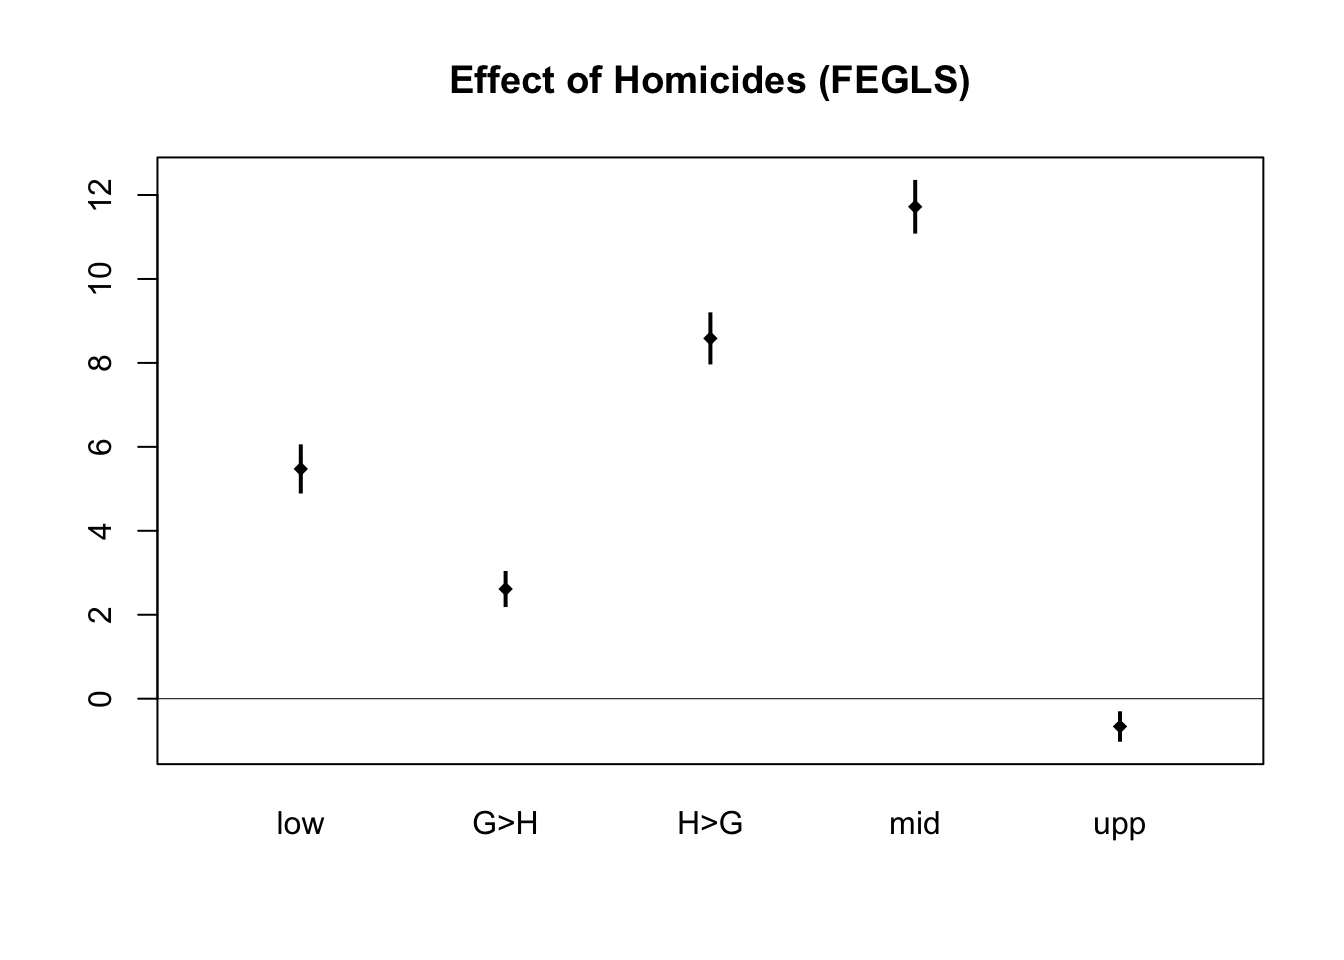
\includegraphics[width=0.67\textwidth]{figures/int_homicides-2.png}
\end{figure}
\begin{figure}[htb]
    \centering
    \caption{Effects of past homicides on current homicides (with violence controls)}
    \label{int_homicides_controls}
    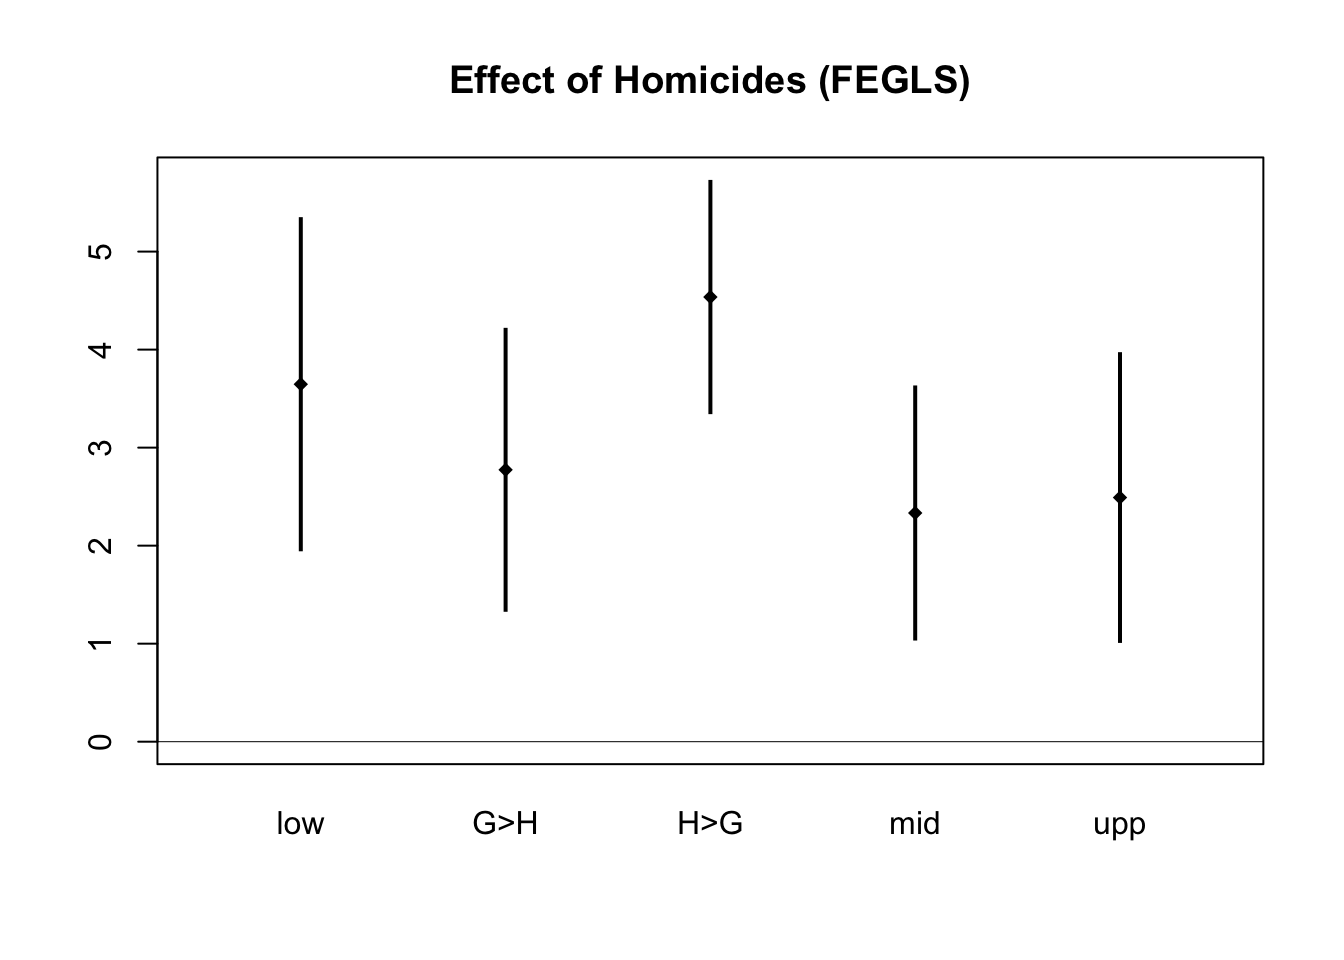
\includegraphics[width=0.67\textwidth]{figures/int_homicides-4.png}
\end{figure}

\clearpage
\subsection{Summary and conclusion}

The panel models summarized in this section examine the framework of vicious and virtuous cycles between health, gender and violence outcomes in several ways.
As in the cross-sectional analyses, simple correlations between individual variables are often, though not always, consistent with the proposed linkages.
The classification groups allow for tests of the effects of particular configurations of health and gender outcomes.
Including the classification indicators often supports \enquote{two-way} vicious cycles in the lowest classification and virtuous cycles in higher classification groups for some measures.
The analyses generally find more supporting correlations in models of health outcomes than in models of gender outcomes.

\enquote{Three-way} cycles are examined with interactions of the classification groups with various measures of violence.
Interaction effects indicate the estimated average change in outcome variables associated with violence in particular classification groups.
Many of these associations are broadly consistent with the vicious and virtuous cycles framework, some contradict it, and many others show no statistically significant effects.
Moreover, whether results are significant often varies by the panel model estimator employed (FE or FEGLS) and whether other types of violence are accounted for in the models.
As in the cross-sectional models investigating violence as independent and dependent variables, the findings are complex.
For instance, the evidence for vicious and virtuous cycles involving internal conflict is weaker in the models of gender outcomes than for health outcomes.
The effects of violent state repression are often consistent with the framework as well, but they are rarely very robust and again favor health over gender outcomes.
Non-state conflict appears to have less systematic effects on gender and health outcomes than the other types of violence, and models of the MYS ratio often contradict expectations.
The evidence for vicious cycles between health outcomes and homicides is also limited.

Even where there is support for vicious and virtuous cycles, it is not clear where the inflection from one to the other occurs. The middle classifications (G>H, H>G, mid) sometimes support vicious cycles and sometimes virtuous ones.

The results of models of violence outcomes are similarly complex.
The models of internal conflict measures provide some evidence supporting the proposed framework.
The findings on violent state repression are mixed.
There is some support for vicious and virtuous cycles in the models of one-sided violence, but also contradictory findings for the latent physical integrity measure.
Models of non-state conflict and deaths provide limited evidence for the proposed framework.
Finally, there is some supportive evidence for homicides.

Despite these complex findings, on balance, there is more support for the framework than against it, but, as in the cross-sectional analyses, strong conclusions are not possible.
Claims about causality are especially not warranted.
These analyses provide broad birds-eye views of aggregate relationships.
However, across many different outcomes and violence measures, there is enough supporting evidence to conclude that vicious and virtuous cycles are hypotheses worthy of deeper theoretical and empirical inquiry.
Ideally, new quantitative research should focus on specific outcomes and build carefully theorized models with observable implications to distinguish, for instance, between vicious and virtuous cycles, short-term and long-term change, and various types and aspects of violence or conflict.

\section{Sequencing analysis}
\label{sequencing}
\paragraph{Oskar Timo Thoms}\ \bigskip

The Lancet-SIGHT Commission is interested not only in whether vicious and virtuous  cycles are at work, but also if and how policy interventions to support gender equality and health equity would be able to nudge societies into virtuous cycles. Toward this end, it is useful to identify pathways of gender and health change to identify entry points and policy levers.
A useful question is: are there particular sequences of improvements in gender and health outcomes that are more likely to break countries out of vicious cycles?
Therefore, another research stream is to map different pathways of change over time, to determine which ones are a) more common and b) likely to lead to improvements.
The present section explains the development of a simple sequencing typology and then relates this typology to outcomes of interest.\footnote{
All the figures in this section and the underlying data work, such as individual country-level pathways, are available at \href{https://timothoms.github.io/LSC-MWG/sequencing.html}{timothoms.github.io/LSC-MWG/sequencing.html}.}

\subsection{Mapping pathways of change and coding a sequencing typology}

The pathways mapping is based on the same four main health (life expectancy and infant mortality ratio) and gender (mean years of schooling ratio and adolescent fertility rate) variables used in the classifications and the large-N regression analyses.\footnote{
As in the previous analyses, the IMR and AFR are inverted such that higher values indicate \enquote{better} outcomes.}
Complete observations for all four measures are available for 182 countries starting in 1970.
Since we are using averages for five-year periods (as in the other analyses in this report), the first period is 1971-1975, and the last is 2011-2015.

As in the construction of the classifications, these variables are scaled to have zero means and standard deviations of one, in order to standardize them but with one important difference.
While for the classifications, the variables were standardized separately for each period (thus comparing the health and gender measures within, but not across, periods), for the present analysis, this standardization is done once for all observations in the dataset, in order to make changes in the different measures comparable over time.\footnote{
Note that the country classifications introduced in \Cref{classifications}, which are available for each period, cannot be used for mapping the pathways of change, because for any given five-year period the classifications are relative to all other countries. In the panel regression analyses, this is useful because it account for the global improvements across the gender and health measures, but it would misrepresents change over time in trend analyses, because an underlying change from one period to the next may not be reflected in the classifications, or a classification may change without a significant change in the underlying health and gender measures.}
The means of the two standardized health variables and of the two standardized gender variables are then calculated and plotted separately for each country, providing the basis for coding the sequencing typology.

\begin{figure}[htbp]
    \centering
    \caption{Pathways (1975-2015) by 1975 classifications (for 1995-2015, see \Cref{sequences_class1995}).}
    \label{sequences_class1975}
    \includegraphics[width=0.45\textwidth]{figures/sequences_class1975_low.pdf}
    \includegraphics[width=0.45\textwidth]{figures/sequences_class1975_G>H.pdf}
    \includegraphics[width=0.45\textwidth]{figures/sequences_class1975_H>G.pdf}
    \includegraphics[width=0.45\textwidth]{figures/sequences_class1975_mid.pdf}
    \includegraphics[width=0.45\textwidth]{figures/sequences_class1975_upp.pdf}
    \includegraphics[width=0.45\textwidth]{figures/sequences_class1975_NA.pdf}
\end{figure}

\Cref{sequences_class1975} overlays the individual country plots, grouped by the classifications for 1971-1975, the first period in the dataset, and \Cref{sequences_class1995} in the appendix provides the pathways from 1991-1995 by the classification for that period.
(A large number of countries is not classified for the former period because many of these come into existence after 1975, or due to missing data in several cases.)
Each coloured line with arrows represents the pathway of a country.
These figures make three key points.
First, almost every country improves on the health and gender outcomes overall from the early 1970s until 2015.
Second, the figures strongly support the notion of ceiling effects when comparing lower with higher classifications.
The pathways in the low classification group show long and spread-out trajectories with much variation in the directions of change, whereas those in the upper classification start with above average health and gender scores and are short and compact, and the pathways in the other classification groups fall in-between these descriptions.
Support for this generalization is still stronger in \Cref{sequences_class1995} in the appendix, which presents the data starting in 1991-1995.
Third, the sub-figures for the G>H and H>G classification groups suggest a subtle difference between the two.
With some exceptions, countries that have stronger  gender than health performance at the outset tend to improve more on health than on gender overall.
This, again, could be due to ceiling effects.
Countries that have stronger health than gender performance at the outset, however, tend to improve similarly on health and gender overall, again with some exceptions.
Ceiling effects may be part of the story, but from a sequencing perspective, gender improvements may also help health improvements more than the other way around.
Further research on this questions would be welcomed.

Based on the individual country pathways (represented by the lines in \Cref{sequences_class1975}) of the combined health and gender measures, I have developed a sequencing typology.
This is a data-driven rather than theory-driven typology.
Considering the direction in a country's health and gender changes in each period, I code whether the two measures improved jointly, or whether one or both declined (which I call setbacks).
It is very rare for both to decline during the same period.
I then summarize the entire sequence by aggregating contiguous periods with the same directions of changes and determine whether any resulting segment is health-led or gender-led, i.e. whether the health or the gender measure improves more than the other (based on the slope) early in the aggregated segment or overall.
In most cases this determination is the same whether based on the first two or three periods of the segment or the entire segment; for edge cases, where these lead to different determinations, the coding for the first periods of a segment is chosen.
The goal is to categorize sequences such that similar pathways are grouped together.
After some initial bivariate analyses of the resulting typology, I further aggregate some categories on the basis of what directions of setbacks occurred.
Given that all countries improved overall, setbacks are a useful distinguishing characteristic, and this aggregation does not lead to loss of variation in the descriptive analyses discussed below.
The complete typology data are provided on the \href{https://timothoms.github.io/LSC-MWG/sequencing.html}{project website}.

\begin{figure}[htbp]
    \centering
    \caption{Sequences, 1975-2015 (for 1995-2015, see \Cref{sequences_typology1995}).}
    \label{sequences_typology1975}
    \includegraphics[width=0.45\textwidth]{figures/sequences_typology1975_2.pdf}
    \includegraphics[width=0.45\textwidth]{figures/sequences_typology1975_4.pdf}
    \includegraphics[width=0.45\textwidth]{figures/sequences_typology1975_3.pdf}
    \includegraphics[width=0.45\textwidth]{figures/sequences_typology1975_5.pdf}
    \includegraphics[width=0.45\textwidth]{figures/sequences_typology1975_1.pdf}
\end{figure}

\Cref{sequences_typology1975} shows the country pathways grouped by the categories of the sequencing typology and notes their frequencies.
(\Cref{sequences_typology1995} in the appendix shows another version of the typology starting with the period of 1991-1995.)
The typology leads to several basic observations about sequences of health and gender change.
First, simple H-led or G-led sequences, where countries improve jointly and continually throughout the entire sequence, are the most common, but H-led sequences are almost twice as common as G-led.
Second, G-led sequences tend to start at higher levels of both the gender and health measures than H-led sequences.
Third, many countries have setbacks on either gender or health, but very few have setbacks on both.
Fourth, sequences with G-setbacks are more numerous than those with H-setbacks.
Finally, setbacks of all types, but particularly G-setbacks, do not necessarily preclude high performance by the end of the sequences.

% \todo[inline]{do i need some more discussion here?}

\subsection{Descriptive analyses}

This section presents distributions of health, gender and violence outcomes broken down by the sequence typology, in order to examine whether different sequences may be associated with different outcomes. Again, such bivariate associations could represent spurious relationships, but they are useful first steps in analyzing whether sequences of change may matter to outcomes.

\subsubsection{Health \& gender change}

\begin{figure}[htbp]
  \centering
  \caption{Distributions of health and gender change per period by sequence (1975-2015)}
  \label{sequences_health_gender}
  \begin{subfigure}[b]{\textwidth}
    \caption{health change}
    \label{sequences_health}
    \includegraphics[width=\textwidth]{figures/sequences_health.pdf}
  \end{subfigure}
  \begin{subfigure}[b]{\textwidth}
    \caption{gender change}
    \label{sequences_gender}
    \includegraphics[width=\textwidth]{figures/sequences_gender.pdf}
  \end{subfigure}
\end{figure}

The difference between the start and end values of the combined health measure used in the pathways mapping for a given country, divided by the number of included periods, provides a simple, comparable measure of the overall health change associated with particular sequences.
\Cref{sequences_health} shows the distribution of this measure for each sequence in the typology.
The boxplots represent the interquartile range and medians, the round points are outliers, and the red diamonds and bars indicate the means with 95\% confidence intervals.
The boxplots do not show statistical effects but where most of the values lie.
The confidence intervals provide a rough indication of whether differences between means are statistically significant.

The figure shows, unsurprisingly, that H-led sequences are associated with more health improvements than G-led sequences and sequences with H-setbacks.
On its face, the association of G-led sequences with limited health improvements may be expected because of how G-led and H-led are defined.
However, it is important to note that segments are coded based only on the relative direction of change, and not based on the overall magnitude of change.
Interestingly, sequences involving H-setbacks or G-setbacks also appear to be associated with more health improvement than G-led sequences.

By contrast, in \Cref{sequences_gender}, which shows the analogous gender change measure, G-led sequences do not have the most gender improvements.
With the unsurprising exception of sequences involving G-setbacks, which are associated with the least gender improvements, these distributions across sequences are closer together than the ones in \Cref{sequences_health}.
Moreover, all but the G-led sequences seem to involve somewhat less overall gender than health change.
No strong conclusions can be drawn from these simple bivariate associations but they are suggestive and invite new analyses.
Some sequences may be more likely to involve greater combined health and gender change than others.
These figures suggest that those sequences are H-led or those with H-setbacks, the latter of which may include G-led and H-led segments.

\begin{figure}[htbp]
    \centering
    \caption{Distribution of path efficiency measure by sequence (1975-2015)}
    \label{sequences_efficiency}
    \includegraphics[width=\textwidth]{figures/sequences_efficiency.pdf}
\end{figure}

\Cref{sequences_efficiency} shows a measure of \enquote{path efficiency.}
This is the Euclidean distance between the start and end values of both the health and gender measures, divided by the total length of all segments in a country's pathway; the closer this measure is to one, the more direct the path from the beginning of a sequence to its end.
Since setbacks imply less efficiency, several of the differences in the figure are as expected, foremost the pathways represented by the H-led and G-led sequences, which are much more efficient than all others, and the inefficient sequence with setbacks on both.
However, the difference between sequences with setbacks is notable: those with G-setbacks are clearly more efficient than those with H-setbacks and those with both setbacks.
One possibility that could be investigated further is that setbacks in health change are more difficult or take longer to recover from than gender setbacks.

\subsubsection{Conflict and violence outcomes}

The remaining figures below show bivariate relationships with several of the violence measures, in order to probe whether certain types of sequences are associated with more violence than others.
The findings are very consistent across different measures of violence, with one partial exception.
Only some of these results are shown here.

\begin{figure}[htbp]
    \centering
    \caption{Internal (incl. internationalized) conflict by sequence (1975-2015)}
    \label{sequences_conflict}
    \includegraphics[width=\textwidth]{figures/sequences_conflict.pdf}
\end{figure}

\Cref{sequences_conflict} employs the same internal conflict data as introduced in \Cref{class1995conflict}, except that here the data are shown for the period 1975-2015.
The ratios between the numbers of countries with and without conflict for the different sequences indicate that G-led sequences are associated with the least conflict and war by far and very little long-term conflict.
Sequences involving H-setbacks or both setbacks have the highest proportions of countries with conflict and war, including long-term.
Interestingly, even H-led sequences are associated with conflict and war for more than half of the countries in that category.
It is possible that this latter association is due to the recovery of health outcomes after conflicts ended.

\begin{figure}[htbp]
    \centering
    \caption{Non-state conflict by sequence (1995-2015)}
    \label{sequences_nsc}
    \includegraphics[width=\textwidth]{figures/sequences_nsc.pdf}
\end{figure}

\Cref{sequences_nsc} shows similar data for non-state conflict. Since these data are available since 1989, this figure (and the next) uses a second version of the sequences typology starting with the 1991-1995 period.
This figure also shows that G-led sequences are associated with violence in the least number of countries, including long-term violence.
Countries with sequences involving H-setbacks have the most non-state conflict.

\begin{figure}[htbp]
    \centering
    \caption{One-sided violence by sequence (1995-2015)}
    \label{sequences_osv}
    \includegraphics[width=\textwidth]{figures/sequences_osv.pdf}
\end{figure}

\Cref{sequences_osv} shows the data on one-sided violence -- such as atrocities against civilians -- for the same period.
G-led sequences are again associated with the smallest numbers of countries with one-sided violence, and in particular violence committed over five years or more.
More than half of countries with sequences involving H-setbacks and even H-led sequences had one-sided violence and high proportions had such violence over more than four years.

\begin{figure}[htbp]
    \centering
    \caption{Distribution of average LPI measure by sequence (1975-2015)}
    \label{sequences_lpi}
    \includegraphics[width=\textwidth]{figures/sequences_lpi.pdf}
\end{figure}

\Cref{sequences_lpi} shows the distributions of another measure of violent state repression, the average latent physical integrity index (LPI).
Recall that this measure was inverted such that higher scores indicate higher levels of state violence.
Once again, G-led sequences are clearly associated with less violence, while sequences involving H-setbacks (or both) have the highest average scores, although the differences between sequences other than G-led are small and cannot be statistically distinguished.
Analogous analyses of V-Dem measures of extra-judicial killings, state torture and societal violence have results very similar to those in \Cref{sequences_lpi}. (These are not shown here, but are available on the \href{https://timothoms.github.io/LSC-MWG/sequencing.html}{project website}.)

\begin{figure}[htbp]
    \centering
    \caption{Distribution of average homicide rates by sequence (1995-2015)}
    \label{sequences_homicides}
    \includegraphics[width=\textwidth]{figures/sequences_homicides.pdf}
\end{figure}

Finally, \Cref{sequences_homicides} shows the distributions of country-level average homicides rates, logged to address skew and make differences easier to discern.
These data have to be used with caution, as they are subject to more missing data than other measures used in this report.
Countries with G-led and H-led sequences have the lowest average homicide rates, and those involving H-setbacks have the highest.
While these differences between sequences are similar to the results for other measures of violence, the finding with respect to G-led sequences is not as strong.

\subsection{Summary}

The descriptive analyses of the sequencing typology suggest that different sequences may be associated with varying health, gender and violence outcomes.
H-led sequences and those with H-setbacks appear to be associated with more overall improvements in health and gender outcomes, but the differences are small and often not statistically distinguishable.
The data also suggest that sequences involving H-setbacks are particularly detrimental to overall change, but this is likely, at least in part, due to greater health than gender changes on the standardized measures for the majority of pathways.
G-led sequences are consistently associated with less violence, while sequences with H-setbacks are associated with the most violence and longer periods of violence.
It is important to note that, violence may occur before or after setbacks; the data presented here does not distinguish their temporal order.
Moreover, H-led sequences are also often linked to much conflict, which may be due to recovery of health outcomes after conflict has ended.

As noted above, no strong conclusions can be drawn from these bivariate associations, but they show sufficient variation in outcomes that new research is warranted to better understand how the pathways of health and gender change may condition the inter-relationships between health, gender and violence.

% \clearpage
% \section{Discussion}
% \paragraph{Oskar Timo Thoms}

% \todo[inline]{needs a discussion section; below are snippets from previous reports}

% While the panel analyses overall still find more evidence of vicious than of virtuous cycles, they do find more support for the latter than the panel analyses in the previous report, and this is largely due to examining the middle classifications. Another objective of examining the middle classifications was to explore whether particular configurations are more likely to result in virtuous cycles: for instance, are those countries that have comparatively better gender outcomes than health outcomes more likely experience virtuous cycles? The evidence from the extensions is not clear on this question. In some cases, the models do show such differences, but these findings are not consistent across outcome and violence variables, making it difficult to generalize.

% Gender and health outcomes are clearly positively correlated with each other.
% This is consistent with the notion that they reinforce each other.

% There is little suggestion of ceiling or convergence effects in the panel. Better health and gender outcomes in one period are associated with improved outcomes in the next period. This difference between the cross-sectional and panel analyses is likely due to the fact that they are differently structured to examine long-term versus shorter-term associations.

% The panel analyses find more support for vicious than virtuous cycles, and that these are more applicable to violence than gender and health outcomes.
% There is some evidence that health and gender outcomes reinforce each other, but the evidence is stronger for health than gender outcomes.

% When considering our classification, which operationalizes the V\&V cycles hypotheses with worst and best combinations of health and gender outcomes, the findings are clear and consistent: the low classification is associated with worse health and gender outcomes across all four variables, but the high classification is never statistically significant. This provides support for vicious cycles between health and gender but not virtuous cycles.

% Few of the violence variables have statistical effects on the gender and health outcomes that are  consistent with the V\&V cycles hypotheses. In fact, many models suggest that violence is, in fact, associated with better health and gender outcomes. (The findings for the AFR are particularly noteworthy in this respect.) A few results are consistent with the V\&V cycles hypotheses, such as the associations of internal war with a worse AFR; internal conflict deaths and one-sided violence with worse infant mortality; the latent physical integrity measure with lower MYS ratios; and, unsurprisingly, homicides and extra-judicial killings with lower life expectancy. However, overall, the health and gender models only support a vicious cycle between health and gender, but do not provide much or consistent evidence for a three-way vicious cycle. Moreover, many models turn up null results.

% The analyses of various violence outcomes more clearly support the theoretical framework, though there are again several contradictory results with respect to the relationship between individual health and gender variables and violence variables, and many null results. ... Like the analyses of health and gender outcomes, these results are not strongly supportive.

% While in bivariate associations, poor health and gender outcomes are clearly associated with more violence on average, the role of violence variables in health and gender outcomes is complex, as violence in one period is sometimes associated with better health and gender outcomes in the next period. This result may seem at odds with V\&V cycles, and points to the need for fuller statistical models based on deeper theoretical work. Moreover, the analyses suggests that different types of violence may matter in different ways.

% However, the evidence is much more consistent and supportive of vicious cycles when using our classifications.

% The panel analyses also consider an alternative conceptualization and operationalization of V\&V cycles, by examining the effects of low and high classifications based on health and gender outcomes. These analyses find clear and consistent support for vicious cycles between health and gender outcomes and in their effects on violence outcomes.

% While we do not find an analogous result for virtuous cycles, we caution that this may be due to our particular conceptualization, which focuses on the extreme ends of our classifications, i.e. the worst and best performers in comparison to all the countries in between, assuming that virtuous and vicious cycles would be most pronounced in these groups. The extensions in this report examine whether variation in the middle group is consistent with the notion of virtuous cycles. Further research may also advance understanding of pathways of change if it considers sequencing.

% While we noted that the lack of evidence for virtuous cycles in the panel analyses may be an artifact of our conceptualization, it is plausible that this result is also due to the different time frames of the analyses. It is possible that virtuous cycles are slow-moving, and thus do not show clear patterns in the panel analyses, while vicious cycles may operate faster.

% Importantly, a three-way vicious cycle between health, gender and violence is strongly supported in many models by the interaction of the lagged violence variables with the low classification; these models examine the effect of previous levels of violence in countries that perform poorly on health and gender on subsequent levels of violence. These interactions are associated with more internal war, internal conflict deaths and civilian deaths, non-state conflict deaths, physical integrity violations, extra-judicial killings and homicides, compared to countries not included in the low and high classifications. These findings strongly suggest that violence begets more violence where countries perform very poorly on both health and gender.

% In models of violence outcomes with interactions between lagged dependent variables with the low and high classifications, we also find strong evidence for three-way vicious cycles, whereby previous violence is associated with renewed (or continued) violence particularly in countries that have very poor health and gender outcomes.

% We also noted that our analyses were limited in several ways.
% First, they examine broad associations and include the same covariates across models.
% However, each of the outcome variables may be better modeled with a different set of covariates, based on different scholarly literatures.
% Such work may shed light, for instance, on the unexpected association between violence and improved adolescent fertility rates.

% This research represents useful ground-clearing for further analyses investigating V\&V cycles between health, gender and violence outcomes. These findings warrant further research.
% Deeper theoretical work and fuller statistical models are needed to address questions arising from these analyses and explore potential pathways from vicious to virtuous cycles. Such research should account for other possible factors, including, for instance, quality of institutions, inequality, functioning of economies, etc.

% \clearpage
\appendix
\part*{Appendix}
\label{appendix}

\section{Additional tables and figures}

\begin{table}[htb]
\centering
\caption{Frequency of classifications in 1975 (143 countries; for 1995, see \Cref{class1995n}).}
\label{class1975n}
\begin{tabular}{lrrrrr}
\toprule
                & \multicolumn{5}{l}{\textbf{Gender}} \\
\textbf{Health} & 1st quintile & 2nd quintile & 3rd quintile & 4th quintile & 5th quintile \\
\midrule
1st quintile    & 19           & 14           & 1            & 0            & 0 \\
2nd quintile    & 7            & 17           & 6            & 2            & 1 \\
3rd quintile    & 0            & 7            & 8            & 3            & 2 \\
4th quintile    & 0            & 1            & 8            & 6            & 8 \\
5th quintile    & 0            & 0            & 2            & 7            & 24 \\
\bottomrule
\end{tabular}
\end{table}

\begin{landscape}
\begin{table}
\footnotesize
\centering
\caption{Country classifications in 1975 (for 1995, see \Cref{class1995}).}
\label{class1975}
\begin{tabular}{p{0.04\linewidth} p{0.17\linewidth} p{0.17\linewidth} p{0.17\linewidth} p{0.17\linewidth} p{0.17\linewidth}}
\toprule
\multicolumn{1}{l}{} & \multicolumn{5}{l}{\textbf{Gender}} \\
\textbf{Health} & Q1 & Q2 & Q3 & Q4 & Q5\\
\midrule
Q1 & Afghanistan; Angola; Bangladesh; Burkina Faso; Central African Republic; Chad; Congo, DRC; Cote d'Ivoire; Equatorial Guinea; Gambia; Guinea; Liberia; Malawi; Mali; Nepal; Niger; Nigeria; Senegal; Sierra Leone & Benin; Bhutan; Bolivia; Burundi; Cambodia; Comoros; Egypt; Guinea-Bissau; Laos; Madagascar; Maldives; Mozambique; Rwanda; Somalia & Haiti &  & \\
\hline
Q2 & Cameroon; Kenya; Pakistan; Sudan; Togo; Uganda; Zambia & Cape Verde; Congo; Eswatini; Gabon; Ghana; Guatemala; India; Indonesia; Iran; Mauritania; Morocco; Nicaragua; Oman; Papua New Guinea; Saudi Arabia; Tanzania; Tunisia & Algeria; El Salvador; Honduras; Myanmar; Peru; Turkey & Mongolia; South Africa & Lesotho\\
\hline
Q3 &  & Iraq; Jordan; Libya; Sao Tome \& Principe; Syria; United Arab Emirates; Zimbabwe & Botswana; China; Colombia; Dominican Republic; Ecuador; Guyana; Mauritius; Mexico & Brazil; Chile; Thailand & Philippines; Samoa\\
\hline
Q4 &  & Kuwait & Bahrain; Brunei; Grenada; Jamaica; Malaysia; Panama; Suriname; Venezuela & Costa Rica; Fiji; Lebanon; Paraguay; Qatar; Trinidad \& Tobago & Albania; Argentina; North Korea; Portugal; South Korea; Sri Lanka; Tonga; Uruguay\\
\hline
Q5 &  &  & Barbados; Cuba & Austria; Bahamas; Bulgaria; Iceland; Romania; Singapore; Taiwan & Australia; Belgium; Canada; Cyprus; Denmark; Finland; France; Greece; Hungary; Ireland; Israel; Italy; Japan; Luxembourg; Malta; Netherlands; New Zealand; Norway; Poland; Spain; Sweden; Switzerland; United Kingdom; United States of America\\
\bottomrule
\end{tabular}
\end{table}
\end{landscape}


\begin{figure}[htbp]
  \centering
  \caption{Pathways (1995-2015, from origin) by 1995 classifications (for 1975-2015, see \Cref{sequences_class1975}).}
  \label{sequences_class1995}
  \includegraphics[width=0.45\textwidth]{figures/sequences_class1995_low.pdf}
  \includegraphics[width=0.45\textwidth]{figures/sequences_class1995_G>H.pdf}
  \includegraphics[width=0.45\textwidth]{figures/sequences_class1995_H>G.pdf}
  \includegraphics[width=0.45\textwidth]{figures/sequences_class1995_mid.pdf}
  \includegraphics[width=0.45\textwidth]{figures/sequences_class1995_upp.pdf}
  \includegraphics[width=0.45\textwidth]{figures/sequences_class1995_NA.pdf}
\end{figure}

\begin{figure}[htbp]
  \centering
  \caption{Sequences, 1995-2015 (for 1975-2015, see \Cref{sequences_typology1975}).}
  \label{sequences_typology1995}
  \includegraphics[width=0.45\textwidth]{figures/sequences_typology1995_2.pdf}
  \includegraphics[width=0.45\textwidth]{figures/sequences_typology1995_4.pdf}
  \includegraphics[width=0.45\textwidth]{figures/sequences_typology1995_3.pdf}
  \includegraphics[width=0.45\textwidth]{figures/sequences_typology1995_5.pdf}
  \includegraphics[width=0.45\textwidth]{figures/sequences_typology1995_1.pdf}
\end{figure}

\end{document}
